\documentclass[a4paper,openany,twoside,final]{book}
% generated by Docutils <http://docutils.sourceforge.net/>
\usepackage{fixltx2e} % LaTeX patches, \textsubscript
\usepackage{cmap} % fix search and cut-and-paste in Acrobat
\usepackage{ifthen}
%\usepackage[T1]{fontenc}
%\usepackage[utf8]{inputenc}
\usepackage{color}
\usepackage{graphicx}
\setcounter{secnumdepth}{-1}
\usepackage{tabularx}

%%% Custom LaTeX preamble
% PDF Standard Fonts
\usepackage{mathptmx} % Times
\usepackage[scaled=.90]{helvet}
\usepackage{courier}

%%% User specified packages and stylesheets
% latex include file for docutils latex writer
% --------------------------------------------
%
% CVS: $Id: style.tex,v 1.1 2004/01/23 21:17:32 faassen Exp $
%
% This is included at the end of the latex header in the generated file,
% to allow overwriting defaults, although this could get hairy.
% Generated files should process well standalone too, LaTeX might give a
% message about a missing file.

% donot indent first line of paragraph.
%\setlength{\parindent}{0pt}
%\setlength{\parskip}{5pt plus 2pt minus 1pt}

% sloppy
% ------
% Less strict (opposite to default fussy) space size between words. Therefore
% less hyphenation.
%\sloppy

% fonts
% -----
% times for pdf generation, gives smaller pdf files.
%
% But in standard postscript fonts: courier and times/helvetica do not fit.
% Maybe use pslatex.
%\usepackage{times}

% pagestyle
% ---------
% headings might put section titles in the page heading, but not if
% the table of contents is done by docutils.
% If pagestyle{headings} is used, \geometry{headheight=10pt,headsep=1pt}
% should be set too.
%\pagestyle{plain}
%
% or use fancyhdr (untested !)
%% \usepackage{fancyhdr}
%% \pagestyle{fancy}
%% \addtolength{\headheight}{\baselineskip}
%% \renewcommand{\sectionmark}[1]{\markboth{#1}{}}
%% \renewcommand{\subsectionmark}[1]{\markright{#1}}
%% \fancyhf{}
%% \fancyhead[LE,RO]{\bfseries\textsf{\thepage}}
%% \fancyhead[LO]{\textsf{\footnotesize\rightmark}}
%% \fancyhead[RE]{\textsc{\textsf{\footnotesize\leftmark}}}
%\fancyfoot[LE,RO]{\bfseries\textsf{\scriptsize Docutils}}
%\fancyfoot[RE,LO]{\textsf{\scriptsize\today}}

% geometry
% --------
% = papersizes and margins
%\geometry{a4paper,twoside,tmargin=1.5cm,
%          headheight=1cm,headsep=0.75cm}

% Do section number display
% -------------------------
%\makeatletter
%\def\@seccntformat#1{}
%\makeatother
% no numbers in toc
%\renewcommand{\numberline}[1]{}


% change maketitle
% ----------------
%\renewcommand{\maketitle}{
%  \begin{titlepage}
%    \begin{center}
%    \textsf{TITLE \@title} \\
%	Date: \today
%    \end{center}
%  \end{titlepage}
%}
% \usepackage[final]{graphicx}
\graphicspath{{./pics/}{./paropt/pics/}}
\usepackage[usenames]{xcolor}
\usepackage{enumitem}
\usepackage[final]{minted}
%\usemintedstyle{emacs}
\usemintedstyle{tango}
%\usemintedstyle{trac} % better (more bold faces}
%\usemintedstyle{manni} % pastel colors
%\usemintedstyle{bw}
\definecolor{mintedbg}{rgb}{0.95,0.95,0.95}
\setminted{breaklines=true,fontsize=\small,funcnamehighlighting=true,python3=true}

%\newminted{prolog}
\protect\newminted[proexp]{text}{style=bw}

% Main style definition
% ---------------------
% ISU standard handbook.
%\usepackage[times,fancybot,firamono]{subook} % looks less good than inconsolata
\usepackage[times,fancybot,inconsolata]{subook} % Looks Good
%\usepackage[times]{subook}

%\setcitestyle{}

% Заменить в коде кой-что на математические формулы
% http://www.tug.org/texlive/Contents/live/texmf-dist/doc/latex/base/alltt.pdf

% Требования к оформлению Типографии ИГУ
% http://lawinstitut.ru/ru/about/services/izdatelstvo/trebovaniya.html
%

% ISU standard monograph (less restrictive and more artistic)
% \usepackage[monograph,mag,times,smalltitles,fancybot,listbib,ptfonts,microtyping]{subook}

% Some artistism for monograph
% ----------------------------
%\makeatletter{}
%\renewcommand\su@chapter@font{\sffamily\sfcpshape\bfseries}
%\renewcommand\su@chapter@font@size{\LARGE}
%\makeatother{}
%\floatname{algorithm}{Процедура}
%\renewcommand{\listalgorithmname}{Список процедур}
%\renewcommand\cftsecnumwidth{5ex}
%\tolerance=5000
%\renewcommand{\chaptername}{Глава}
%\usepackage[final]{hyperref}

\definecolor{mygreen}{rgb}{0,0.6,0}
\definecolor{mygray}{rgb}{0.5,0.5,0.5}
\definecolor{mymauve}{rgb}{0.58,0,0.82}


\usepackage{tikz}
\usetikzlibrary{arrows,arrows.meta,shapes}
\usetikzlibrary{shadows}
\newcommand*\keystroke[1]{%
  \tikz[baseline=(key.base)]
    \node[%
      draw,
      fill=white,
      drop shadow={shadow xshift=0.25ex,shadow yshift=-0.25ex,fill=black,opacity=0.75},
      rectangle,
      rounded corners=4pt,
      inner sep=1pt,
      line width=0.7pt,
      font=\footnotesize\sffamily
    ](key) {~#1~\strut}%
  ;%
}

\long\def\rem#1{}
%\def\AR{{\em Прим.~авторов~пособия}}
\def\emphbib#1{#1}
\newenvironment{questions}{\subsubsection*{Вопросы для самопроверки}\begin{enumerate}\itemsep0pt minus 0.3pt\parskip0pt plus 0.3pt}{\end{enumerate}}

\newtheorem{example}{Пример}[chapter]
\hypersetup{
    bookmarks=true,         % show bookmarks bar?
    unicode=true,           % non-Latin characters in Acrobat’s bookmarks
    pdftoolbar=true,        % show Acrobat’s toolbar?
    pdfmenubar=true,        % show Acrobat’s menu?
    pdffitwindow=false,     % window fit to page when opened
    pdfstartview={FitH},    % fits the width of the page to the window
    pdftitle={Компьютерные науки, часть 4},    % title
    pdfauthor={Евгений Александрович Черкашин},     % author
    pdfsubject={Методическое пособие},   % subject of the document
    pdfcreator={EMACS-24.4:AuCTeX},   % creator of the document
    pdfproducer={LuaLaTeX}, % producer of the document
    pdfkeywords={Искусственный интеллект} {Логическое
      программирование} {Планирование действий} {Удовлетворение
      ограничений} {Компьютерная алгебра} {Принцип максимума} {Оптимальное управление}, % list of keywords
    pdfnewwindow=true,      % links in new window
    colorlinks=true,       % false: boxed links; true: colored links
    linkcolor=[rgb]{0 0.4 0.1},          % color of internal links (black)
    citecolor=blue,        % color of links to bibliography
    filecolor=black,      % color of file links
    urlcolor=[rgb]{0.3 0.0 0.3}           % color of external links
}

%\renewcommand{\headrulewidth}{1pt}

\clubpenalty=3000
\widowpenalty=3000
%\brokenpenalty=10000
%\floatingpenalty=10000

%% \setdefaultlanguage{russian}
%% \setmainlanguage{russian}
%% \setotherlanguage{english}

%\newenvironment{mygroup}{}{}

\renewcommand\baselinestretch{1.5} % FIXME Какой интервал тут реально получится?
\newcommand{\eeng}[1]{\emph{\foreignlanguage{english}{#1}}}

\definecolor{rclr}{rgb}{0.5,0.1,0.1}
\definecolor{eclr}{rgb}{0,0.5,0.5}
\colorlet{acolor}{blue}
\colorlet{rcolor}{red}
\definecolor{ncolor}{rgb}{0.5,0.5,0.1}
\newcommand{\aaa}[2][acolor]{\noindent\textcolor{eclr}%
{+\ [}\textcolor{#1}{#2}\textcolor{eclr}{]}}
\newcommand{\rrr}[2][rcolor]{\noindent%
\textcolor{eclr}{-\ [}\textcolor{#1}{#2}\textcolor{eclr}{]}}
\newcommand{\nnn}[2][ncolor]{\noindent%
\textcolor{eclr}{!\ [}\textcolor{#1}{#2}\textcolor{eclr}{]}}
\newcommand{\goforth}[1]{$\,\hookrightarrow$\pageref{#1}}

% \begin{figure}
%   \centering
%   \def\svgwidth{\columnwidth}
%   \includesvg{image}
% \end{figure}

\parskip=0pt plus 0.3pt
\renewcommand{\chaptername}{} % for ISU Handbooks
\renewcommand{\refname}{Рекомендуемая литература} % ... also
\renewcommand{\bibname}{\refname}


\renewcommand{\baselinestretch}{1.0}

%%% Fallback definitions for Docutils-specific commands

% providelength (provide a length variable and set default, if it is new)
\providecommand*{\DUprovidelength}[2]{
  \ifthenelse{\isundefined{#1}}{\newlength{#1}\setlength{#1}{#2}}{}
}

% admonition (specially marked topic)
\providecommand{\DUadmonition}[2][class-arg]{%
  % try \DUadmonition#1{#2}:
  \ifcsname DUadmonition#1\endcsname%
    \csname DUadmonition#1\endcsname{#2}%
  \else
    \begin{center}
      \fbox{\parbox{0.9\textwidth}{#2}}
    \end{center}
  \fi
}

% docinfo (width of docinfo table)
\DUprovidelength{\DUdocinfowidth}{0.9\textwidth}
% numeric or symbol footnotes with hyperlinks
\providecommand*{\DUfootnotemark}[3]{%
  \raisebox{1em}{\hypertarget{#1}{}}%
  \hyperlink{#2}{\textsuperscript{#3}}%
}
\providecommand{\DUfootnotetext}[4]{%
  \begingroup%
  \renewcommand{\thefootnote}{%
    \protect\raisebox{1em}{\protect\hypertarget{#1}{}}%
    \protect\hyperlink{#2}{#3}}%
  \footnotetext{#4}%
  \endgroup%
}

% sidebar (text outside the main text flow)
\providecommand{\DUsidebar}[2][class-arg]{%
  \begin{center}
    \colorbox[gray]{0.80}{\parbox{0.9\textwidth}{#2}}
  \end{center}
}

% title for topics, admonitions, unsupported section levels, and sidebar
\providecommand*{\DUtitle}[2][class-arg]{%
  % call \DUtitle#1{#2} if it exists:
  \ifcsname DUtitle#1\endcsname%
    \csname DUtitle#1\endcsname{#2}%
  \else
    \smallskip\noindent\textbf{#2}\smallskip%
  \fi
}

% titlereference role
\providecommand*{\DUroletitlereference}[1]{\textsl{#1}}

% hyperlinks:
\ifthenelse{\isundefined{\hypersetup}}{
  \usepackage[colorlinks=true,linkcolor=blue,urlcolor=blue]{hyperref}
  \urlstyle{same} % normal text font (alternatives: tt, rm, sf)
}{}
\hypersetup{
  pdftitle={Компонентное программирование в Python},
}

%%% Title Data
%\title{\phantomsection%
%  Компонентная архитектура Python и Zope%
%  \label{zope}}
%\author{Е.~А.~Черкашин, М.~Байджу}
%\date{}

%%% Body
\newcommand\e[1]{#1}
\renewcommand\chaptername{Глава}
\begin{document}
%\maketitle

\begin{titlepage}
\thispagestyle{empty}
\begin{center}{\small{}
Министерство образования и науки
Российской федерации \\
%Федеральное государственное бюджетное образовательное\\
%учреждение высшего профессионального образования\\
%<<Иркутский государственный технический университет>>\\[2ex]
%Федеральное государственное бюджетное образовательное\\
%учреждение высшего профессионального образования\\
Иркутский национальный исследовательский технический университет\\[1ex]
    Учреждение Российской академии наук \\
<<Институт динамики систем и теории управления им.~В.~М.~Матросова\\
Сибирского отделения РАН>>
}
\vfill
\hbox to \linewidth{\hfill\bfseries Е.~А.~Черкашин, М.~Байджу\hfill}
 \vspace{2em}
{\large\bfseries Компонентное программирование в Python%
}\\
 \vspace{2em}
{Учебное пособие}
\vfill
%\vfill
\vfill
 \textbf{Иркутск 2016}
\end{center}
\end{titlepage}



% Docinfo
% \begin{center}
% \begin{tabularx}{\DUdocinfowidth}{lX}
% \textbf{Авторы}: &
% Е.~А.~Черкашин, М.~Байджу
% \\
% \textbf{Версия}: &
% 0.5.8
% \\
% \textbf{Печатный экземпляр на англ. языке}: &
% \url{http://www.lulu.com/content/1561045}
% \\
% \textbf{PDF-версия оригинала на англ.}: &
% \url{http://www.muthukadan.net/docs/zca.pdf}
% \\
% \textbf{Перевод}: &
% канд. техн. наук. Черкашин Евгений Александрович
% \\
% \textbf{Версия перевода}: &
% 0.1
% \\
% \end{tabularx}
% \end{center}

% Copyright (C) 2007,2008,2009 Baiju M <baiju.m.mail AT gmail.com>.

% Разрешается копировать, распространять и/или вносить изменения в этот
% документ при соблюдении условий лицензии GNU Free Documentation
% License, версия 1.2 или по вашему желанию какой-либо поздней версии,
% официально опубликованной Фондом свободного программного обеспечения
% (Free Software Foundation).

% Исходный код программ, приведенный в тектсе книги, распространяется
% при соблюдении положений лицензии Zope Public License, версии 2.1
% (ZPL).

% ИСХОДНЫЙ КОД ПРОГРАММ В ЭТОМ ДОКУМЕНТЕ И САМ ДОКУМЕНТ ПРЕДОСТАВЛЯЮТСЯ
% В ТОМ ВИДЕ, КАК ОН ПРИВЕДЕН В ТЕКСТЕ (\textquotedbl{}КАК ЕСТЬ\textquotedbl{}). АВТОР НЕ ПРИНИМАЕТ
% НА СЕБЯ НИКАКИХ ГАРАНТИЙНЫХ ОБЯЗАТЕЛЬСТВ, КАК ЯВНО ВЫРАЖЕННЫХ, ТАК И
% ПОДРАЗУМЕВАЕМЫХ, В ТОМ ЧИСЛЕ ПОДРАЗУМЕВАЕМЫЕ ГАРАНТИИ ОБЕСПЕЧЕНИЯ
% ПРАВА ВЛАДЕНИЯ, ТОВАРНОГО СОСТОЯНИЯ ПРИ ПРОДАЖЕ, ПРОТИВОДЕЙСТВИЯ
% НАРУШЕНИЯМ ЛИЦЕНЗИОННЫХ СОГЛАШЕНИЙ, А ТАКЖЕ ПРИГОДНОСТИ ДЛЯ
% ИСПОЛЬЗОВАНИЯ В КОНКРЕТНЫХ ЗАДАЧАХ.

% \DUsidebar{
% \DUtitle[title]{Благодарности}

% Много людей помогли мне написать эту книгу.  Первоначальный
% манускрипт отрецензирован моим коллегой Брэдом Алленом (Brad Allen).
% Когда я объявил о книге в моем блоге, общественность вдохновила меня
% продолжить ее совершенствование.  Кент Тенни (Kent Tenney) творчески
% обработал практически все разделы книги, кроме того, он переписал
% основной пример - приложение.  Многие присылали мне замечания,
% исправления ошибок и недочетов, в том числе Лоренсо Санчеса (Lorenzo Gil
% Sanchez), Михаэль Гаубенвалнера (Michael Haubenwallner), Нандо
% Куинтан (Nando Quintana), Стефани Кляйн (Stephane Klein), Тим Кук
% (Tim Cook), Камал Джилл (Kamal Gill) и Томас Герв (Thomas
% Herve).  Лоренсо перевел книгу на испанский язык, а Стефани на
% французский.  Огромное всем спасибо!

% При переводе на русский язык неоценимую помощь оказал Антон
% Кочнев. Спасибо ему за это.
% }

\newpage{}
\begin{mygroup}
\thispagestyle{empty}
\noindent УДК 681.3.06 (075.8)\\ % (075.8) = Handbook
% \noindent УДК~165:681.3.06+62-52\\
% Программирование для ЭВМ--Учебники и пособия для вузов
\noindent ББК 32.973-01я73\\ % я73 - Учебник для вузов -01=
% 86.4 = Логика
% 32.973 = Программное обеспечение
% 32.813 = Искусственный интеллект
% -01 =
% ББК 87.4:32.973-01+32.813\\ % monograph
\noindent\mbox{}\hspace{2em}Ч-48 % Author Sign (Авторский знак)
\vfill
\begin{center}\small
Рекомендовано к изданию редакционно-издательским советом ИРНИТУ\\
%\bfseries Издание выходит в рамках Программы\\
%стратегического развития ФГБОУ ВПО <<ИГУ>>\\
%на 2012--2016 гг., проект Р121-02-001%
%}
\end{center}
\vspace{1ex}
\begin{center}\small
\textbf{Рецензенты:} \\
зав.~лаб.~4.1.~ИДСТУ СО РАН, канд.~техн.~наук~{\em А.~Е.~Хмельнов},\\
ст.~преп.~каф.~ИС.~ИМЭИ~ИГУ, канд.~физ.-мат.~наук~{\em И.~А.~Казаков}
\end{center}
\vfill
\noindent\begin{minipage}[t]{2em}
\noindent\mbox{}\\
Ч-48
\end{minipage}%
\begin{minipage}[t]{0.95\linewidth}
\setlength{\parindent}{5ex}
\noindent{\bfseries Черкашин~Е.~А.}

Компонентное программирование в Python\,{}: учеб.~пособие\,/~Е.~А.~Черкашин, М.~Байджу~-- Иркутск\,: Изд"=во ИРНИТУ, 2016.~-- \pageref{lastpage}~c.

{\bfseries \e{ISBN 978-5-9624-ХХХ-Х}}
\vspace{2ex}

\begingroup\small\parskip0pt
\vspace{1ex}

%особие соответствует требованиям ФГОС-3

В пособии представлены материалы лекций и задания лабораторных работ по курсу <<Сетевые операционные системы>> Института кибернетики им.~Е.~И.~Попова Иркутского государственного технического университета, тема  «Компонентное проектирование распределенных систем», направление подготовки магистра~-- 09.04.01.  Задача курса состоит в развитии навыков проектирования сложных программных комплексов на основе формального описания его компонент, их регистрации в репозитории компонент, конфигурировании программной системы.

Предполагаемая аудитория пособия: студенты, магистранты, аспиранты и молодые специалисты инженерных специальностей, связанных с программированием распределенных систем, серверов, сетей распределенной обработки информации, прикладных пакетов. Материал пособия адаптируем к курсам <<Технологии программирования>>, <<Открытые системы>>.

\mbox{}
\endgroup
\end{minipage}
\mbox{}\hspace{0.7\linewidth}
\begin{minipage}{0.3\linewidth}\small
\noindent УДК 681.3.06 (075.8)\\
\noindent ББК 32.973-01я73
\end{minipage}
\vfill
\vfill
\noindent\begin{minipage}[t]{0.35\linewidth}\small
\noindent \e{ISBN 978-5-9624-ХХХХ-Х}
\end{minipage}%
\begin{minipage}[t]{0.65\linewidth}\small
\begin{itemize}
\setlength{\itemsep}{-0.5ex}
\setlength{\parsep}{0pt}
\item[\copyright{}] Черкашин~Е.~А., Байджу~М., 2016
%\item[\copyright{}] ФГБОУ ВПО <<ИГУ>>, 2015
\item[\copyright{}] ФГБОУ ВПО ИРНИТУ, 2016
\item[\copyright{}] ФГБУН ИДСТУ СО РАН, 2016
\end{itemize}
\end{minipage}
\end{mygroup}
\newpage{}
\phantomsection\label{contents}
\pdfbookmark[1]{Contents}{contents}
\tableofcontents



\chapter{Введение%
  \label{id1}%
}


%\section{Введение%
%  \label{id2}%
%}

Разработка больших программных систем практически всегда является сложным и трудоемким занятием, где объектно"=ориентированный подход к анализу, проектированию и реализации (программированию) достаточно хорошо себя зарекомендовал.  Проектирование и разработка программного обеспечения, использующая компонентный подход, становятся все более и более популярным методом проектирования.  Компонентный подход и unit"=тестирование позволяет достаточно просто разрабатывать и поддерживать программные системы.  Существует много различных программных инфраструктур и инструментариев разработчика (framework), реализующих компонентное проектирование для разных языков программирования и их средах, некоторые даже не зависят от какой"=либо конкретной среды разработки.  Примерами выступают COM, разработанный Microsoft, и XPCOM - Mozilla.

\textbf{Компонентная архитектура Zope (Zope Component Architecture, ZCA)}~-- это одна из таких инфраструктур, разработанная для среды программирования Python, реализующая компонентный подход к проектированию и программированию.  Он позволяет проектировать большие программные системы в среде программирования Python.  И делает это совсем не плохо.  Компонентная архитектура ZCA не требует для своего использования сервера приложений Zope, ZCA может использоваться в разработке любого Python"=приложения.  Справедливо было бы назвать ZCA \DUroletitlereference{компонентной архитектурой Python} (Python Component Architecture).

ZCA позволяет использовать объекты Python эффективно.  \DUroletitlereference{Компоненты}~-- это объекты, которые легко использовать повторно, а к интерфейсам этих компонент можно получить полный доступ во время исполнения программы (introspection).  \DUroletitlereference{Интерфейс}~-- это объект, который описывает как следует взаимодействовать с конкретной компонентой.  Другими словами, компонента \DUroletitlereference{обслуживает сервисы} (provides)\DUfootnotemark{id3}{fn1}{1}, определенные в интерфейсе.  Компонента \DUroletitlereference{реализуется} (implemented) в виде класса (class) или другого исполняемого объекта (callable object).  И не важно, как реализована эта компонента, а вот что важно~-- это то, что она соответствует \DUroletitlereference{требованиям}, определенным в интерфейсе (interface contract).  При помощи ZCA сложность системы распределяется между множеством кооперирующихся компонент.  Механизм такой кооперации обеспечивается двумя базовыми разновидностями компонент в ZCA: \DUroletitlereference{адаптером} (adapter) и \DUroletitlereference{утилитой} (utility).

\begin{quote}

  \DUfootnotetext{fn1}{id3}{1}{\phantomsection\label{fn1}%
    Примечание переводчика~-- слово \textquotedbl{}provides\textquotedbl{} в исходном английском варианте текста имеет несколько основных вариантов перевода: \textquotedbl{}обеспечивает\textquotedbl{}, \textquotedbl{}реализует\textquotedbl{}, \textquotedbl{}обслуживает\textquotedbl{}, \textquotedbl{}оснащает\textquotedbl{}, \textquotedbl{}оборудует\textquotedbl{} и \textquotedbl{}образует собой\textquotedbl{}. Слово \textquotedbl{}реализует\textquotedbl{} уже зарезервировано для перевода слова \textquotedbl{}implements\textquotedbl{}, которое подразумевает программный код языка программирования Python реализующий методы в интерфейсе.  Слово \textquotedbl{}обеспечивать\textquotedbl{} в данном контексте имеет слишком абстрактный смысл, включающий всю семантику, образуемыми представленными вариантами перевода.  Поэтому более менее точным и подходящим для цели изложения материала в данной книге вариантом перевода \textquotedbl{}provides\textquotedbl{} видится слово \textquotedbl{}обслуживает\textquotedbl{} в предположении, что в объекте (экземпляре класса) исполняется программный код метода, которому передано управление через данный интерфейс.  Варианты \textquotedbl{}оснащает\textquotedbl{}, \textquotedbl{}оборудует\textquotedbl{} и др. по мнению переводчика относятся не ко времени исполнения программного кода, а представляют собой статический аспект исходного слова \textquotedbl{}provides\textquotedbl{}.  }

\end{quote}

ZCA распределен между тремя базовыми пакетами:

\begin{quote}

\begin{itemize}

\item \texttt{zope.interface}, используемый для определения (задания)
интерфейсов компонент.

\item \texttt{zope.event}, поддерживающий базовый механизм порождения и
обработки событий.

\item \texttt{zope.component}, обеспечивающий порождение и регистрацию
компонент, а также их предоставление приложению по запросу.

\end{itemize}

\end{quote}

Обращаю внимание, что ZCA сам по себе не является компонентой и не состоит из них, ZCA скорее механизм и библиотека для создания, регистрации и обеспечения доступа из программного кода приложения к зарегистрированным компонентам.  В продолжение к предыдущему замечанию, \DUroletitlereference{Адаптер}~-- это, как правило, обычный класс Python или фабрика классов (factory), а \DUroletitlereference{утилита}~-- это обычный запускаемый объект в среде исполнения Python.

Среда ZCA разрабатывается как одна из задач проекта Zope 3.  Как сказано выше ZCA является чисто питоновским фреймворком, и может использоваться в любых приложениях Python.  В настоящее время ZCA активно используется в проектах Zope 3, Zope 2 и Grok.  Существуют и другие приложения, в т.~ч. и неинтернет"=приложения, использующие ZCA\DUfootnotemark{id4}{projects}{2}.

\DUfootnotetext{projects}{id4}{2}{\phantomsection\label{projects}%
\url{http://wiki.zope.org/zope3/ComponentArchitecture}
}


\section{Краткая история проекта%
  \label{id5}%
}

Проект ZCA начался в 2001 году и являлся частью проекта Zope 3.  Причиной появления Zope 3 послужил анализ опыта, полученного при разработке комплексных программных систем на основе Zope 2.  Джим Фултон (Jim Fulton) стал лидером проекта.  Сообщество разработчиков, внесших свой вклад в дизайн и реализацию ZCA, возглавляется известными инженерами: Стефаном Рихтером (Stephan Richter), Филиппом фон Вайтершаусеном (Philipp von Weitershausen), Гвидо ван Россумом (Guido van Rossum), известным также как \emph{Python BDFL}, Тресом Сивером (Tres Seaver), Филиппом Дж Эби (Phillip J Eby) и Мартином Фаассеном (and Martijn Faassen).

В начале проекта Zope 3 в ZCA существовали дополнительные компоненты~-- \DUroletitlereference{сервисы} (services) и \DUroletitlereference{представления} (views), но в процессе разработки оказалось, что \DUroletitlereference{утилиты} заменяют полностью сервисы, а \DUroletitlereference{мультиадаптеры}~-- представления.  В настоящее время ZCA включает в себя небольшой набор базовых компонент: \DUroletitlereference{утилиты}, \DUroletitlereference{адаптеры}, \DUroletitlereference{подписчики} (subscribers) и \DUroletitlereference{обработчики} (handlers).  На самом деле \DUroletitlereference{подписчики} и \DUroletitlereference{обработчики}~-- это два особых вида адаптеров.

В процессе подготовки версии Zope 3.2 Джим Фултон предложил значительно упростить среду компонентного программирования ZCA\DUfootnotemark{id6}{proposal}{3}.  В результате этого появился новый общий интерфейс \DUroletitlereference{IComponentRegistry}, позволяющий регистрировать как локальные так и глобальные компоненты.

\DUfootnotetext{proposal}{id6}{3}{\phantomsection\label{proposal}%
\url{http://wiki.zope.org/zope3/LocalComponentManagementSimplification}
}

В результате от пакета \texttt{zope.component} перестал зависеть достаточно длинный список других пакетов, при этом оставшиеся зависимости не относились напрямую к разработке приложений Zope 3.  На конференции PyCon 2007 Джим Фултон предложил включить в пакет \DUroletitlereference{setuptools} функцию \DUroletitlereference{extras\_require}, чтобы усилить уровень изолированности базового набора функций ZCA от вспомогательных функций\DUfootnotemark{id7}{extras}{4}.

\DUfootnotetext{extras}{id7}{4}{\phantomsection\label{extras}%
\url{http://peak.telecommunity.com/DevCenter/setuptools\#declaring-dependencies}
}

В марте 2009, Трес Сивер окончательно устранил зависимости пакета от \texttt{zope.deferredimport} и \texttt{zope.proxy}.

Теперь проект ZCA является независимым со своим собственным планом выпусков и репозиторием Subversion.  Проект как и прежде является составляющей частью среды разработки интернет"=приложений Zope\DUfootnotemark{id8}{framework}{5}.  При этом ошибки и недочеты, выявляемые в ZCA, все еще публикуются на сайте системы отслеживания ошибок проекта Zope 3\DUfootnotemark{id9}{bugs}{6}.  Кроме того, основной список рассылки \DUroletitlereference{zope"=dev} все еще используется для информационного обмена разработчиками ZCA\DUfootnotemark{id10}{discussions}{7}.  Существует также список рассылки, предназначенный для пользователей Zope 3, \DUroletitlereference{zope3"=users}, в котором можно получить ответы на вопросы о ZCA\DUfootnotemark{id11}{z3users}{8}.

\DUfootnotetext{framework}{id8}{5}{\phantomsection\label{framework}%
\url{http://docs.zope.org/zopeframework/}
}

\DUfootnotetext{bugs}{id9}{6}{\phantomsection\label{bugs}%
\url{https://bugs.launchpad.net/zope3}
}

\DUfootnotetext{discussions}{id10}{7}{\phantomsection\label{discussions}%
\url{http://mail.zope.org/mailman/listinfo/zope-dev}
}

\DUfootnotetext{z3users}{id11}{8}{\phantomsection\label{z3users}%
\url{http://mail.zope.org/mailman/listinfo/zope3-users}
}


\section{Установка%
  \label{id12}%
}

Пакеты \texttt{zope.component}, \texttt{zope.interface} и \texttt{zope.event} являются ядром Компонентной архитектуры Zope.  Они содержат технические средства для определения, регистрации и поиска компонент.  Пакет \texttt{zope.component} и пакеты, зависящие от него, доступны в формате egg на сайте Python Package Index (PyPI)\DUfootnotemark{id13}{pypi}{9}.

\DUfootnotetext{pypi}{id13}{9}{\phantomsection\label{pypi}%
Хранилище пакетов Python: \url{http://pypi.python.org/pypi}
}

Проще всего устанавливать \texttt{zope.component} и его зависимые пакеты при помощи программы \DUroletitlereference{easy\_install}\DUfootnotemark{id14}{easyinstall}{10}

\begin{minted}{bash}
$ easy_install zope.component
\end{minted}

\DUfootnotetext{easyinstall}{id14}{10}{\phantomsection\label{easyinstall}%
\url{http://peak.telecommunity.com/DevCenter/EasyInstall}
}

Программ загружает \texttt{zope.component}, его зависимые пакеты с сайта PyPI и устанавливает все как библиотеки интерпретатора Python.

С другой стороны, можно загрузить \texttt{zope.component} и зависящие от него пакеты с сайта PyPI и, затем, самостоятельно установить их.  Установку пакетов следует производить в порядке, описанном ниже.  В операционной системе Windows необходимо загрузить двоичные сборки следующих пакетов.

\begin{quote}
\newcounter{listcnt0}
\begin{list}{\arabic{listcnt0}.}
{
\usecounter{listcnt0}
\setlength{\rightmargin}{\leftmargin}
}

\item \texttt{zope.interface};

\item \texttt{zope.event};

\item \texttt{zope.component}.
\end{list}

\end{quote}

Для установки загруженных пакетов можно, как и раньше, использовать команду \texttt{easy\_install}, при этом передавая в качестве параметра устанавливаемые пакеты, аналогично двоичным egg"=пакетам.  Команда позволяет все пакеты указывать одновременно в одной командной строке.

\begin{minted}{bash}
$ easy_install /path/to/zope.interface-3.x.x.tar.gz
$ easy_install /path/to/zope.event-3.x.x.tar.gz
$ easy_install /path/to/zope.component-3.x.x.tar.gz
\end{minted}

Кроме того, все пакеты можно разархивировать и установить по одному, например:

\begin{minted}{bash}
$ tar zxvf /path/to/zope.interface-3.x.x.tar.gz
$ cd zope.interface-3.x.x
$ python setup.py build
$ python setup.py install
\end{minted}

В результате исполнения этих команд ZCA устанавливается как общесистемная библиотека Python в директорий \texttt{site"=packages}, что, иногда, создает некоторые проблемы.  Джим Фултон в списке рассылки Zope 3 не рекомендовал устанавливать пакеты в общесистемном директории Python\DUfootnotemark{id15}{systempython}{11}.  Их рекомендуется устанавливать в виртуальное окружение, создаваемое помощи программы \texttt{virtualenv}, или пакета \texttt{zc.buildout}.  Такой подход предоставляет возможности для проведения экспериментов с пакетами Python.  Кроме того, в виртуальном окружении удобно развертывать уже готовые приложения.

\DUfootnotetext{systempython}{id15}{11}{\phantomsection\label{systempython}%
\url{http://article.gmane.org/gmane.comp.web.zope.zope3/21045}
}


\section{Подготовка виртуального окружения%
  \label{id16}%
}

Существует множество популярных подходов к настройке изолированного виртуального окружения для среды программирования Python, удобного для разработки приложений.  Наиболее популярные~-- это пакет \texttt{virtualenv}, разработанный Яном Бикингом (Ian Biking) и пакет \texttt{zc.buildout}, разработанный Джимом Фултоном.  Оба этих пакета можно использовать и одновременно.

\begin{minted}{bash}
virtualenv
\end{minted}
Пакет \texttt{virtualenv} устанавливается при помощи команды \texttt{easy\_install}:

\begin{minted}{bash}
$ easy_install virtualenv
\end{minted}

Затем создается новое окружение:

\begin{minted}{bash}
$ virtualenv --no-site-packages myve
\end{minted}

Команда \texttt{easy\_install} создает новое окружение в директории \texttt{myve}.  Теперь в этот директорий можно установить \texttt{zope.component} и пакеты, которые от него зависят.  Команду необходимо запускать с использованием префикса \texttt{myve/bin}

\begin{minted}{bash}
$ cd myve
$ ./bin/easy_install zope.component
\end{minted}

Теперь можно попробовать импортировать пакеты \texttt{zope.interface} и \texttt{zope.component} из командной строки интерпретатора \texttt{python}, который находится в директории \texttt{myve/bin}:

\begin{minted}{bash}
$ ./bin/python
\end{minted}

После запуска Python выведет на экран его стандартное приглашение для ввода команд и выражений.  В командной строке будем выполнять программный код, приводимый в книге.

\begin{minted}{bash}
zc.buildout
\end{minted}

При помощи пакета \texttt{zc.buildout} и \DUroletitlereference{рецепта} (recipe) \texttt{zc.recipe.egg} создаются специализированные версии интерпретатора Python с встроенными egg"=пакетами.  Для этого необходимо установить пакет \texttt{zc.buildout} при помощи команды \texttt{easy\_install}, имеет смысл установить этот пакет также внутри виртуального окружения.

Чтобы создать новое buildout"=окружение для проведения экспериментов с egg"=пакетами Python, сначала создайте для него новый директорий, и, затем, создайте в нем так называемое buildout"=окружение при помощи команды \texttt{buildout init}:

\begin{minted}{bash}
$ mkdir mybuildout
$ cd mybuildout
$ buildout init
\end{minted}

Теперь директорий \texttt{mybuildout}~-- новое buildout"=окружение.  Настройки окружения по умолчанию хранятся в файле \DUroletitlereference{buildout.cfg}.  Сначала в нем содержится следующий текст:

\begin{minted}{ini}
[buildout]
chapters =
\end{minted}

Надо внести в настройки следующие изменения:

\begin{minted}{ini}
[buildout]
chapters = py

[py]
recipe = zc.recipe.egg
interpreter = python
eggs = zope.component
\end{minted}

Запуск команды \texttt{buildout} из директория \texttt{mybuildout/bin} (без аргументов) создаст копию интерпретатора Python в директории \texttt{mybuildout/bin}:

\begin{minted}{bash}
$ ./bin/buildout
$ ./bin/python
\end{minted}

Последняя команда выведет на экран приглашение Python, в котором будем запускать приводимый далее в книге программный код.


\chapter{Пример задачи%
  \label{id17}%
}


Рассмотрим приложение, предназначенное для регистрации постояльцев в гостинице.  В среде Python его можно реализовать множеством способов.  Сначала кратко рассмотрим процедурный подход, затем перейдем к объектно"=ориентированному программированию.  После анализа результатов дизайна и реализации задачи при помощи объектно"=ориентированного подхода, рассмотрим как данная задача решается при помощи классических шаблонов проектирования (паттернов проектирования, design patterns) \DUroletitlereference{адаптер} и \DUroletitlereference{интерфейс}.  Таким образом у вас появится начальное представление о возможностях Компонентой архитектуры Zope.


\section{Процедурный подход%
  \label{id19}%
}

Модуль хранения данных~-- очень важный момент в разработке приложений.  В рассматриваемом примере будем использовать словарь (dictionary) языка Python в качестве такой системы хранения.  Каждой записи соответствует сгенерированный уникальный ключ (ID).  Ключ ассоциируется со значением, которое тоже будет словарем и будет содержать данные о бронировании комнаты в гостинице.

\begin{minted}{ex}
    bookings_db = {} #key - уникальный идентификатор (ID), value - данные брони
\end{minted}

В реализации системы нужна, как минимум, функция, которой передаются данные о бронировании, и функция, которая генерирует уникальное значение ID ключа для ассоциации с данными брони.

Сгенерировать значение ключа можно следующим образом:

\begin{minted}{python}
    def get_next_id():
        db_keys = bookings_db.keys()
        if db_keys == []:
            next_id = 1
        else:
            next_id = max(db_keys) + 1
        return next_id
\end{minted}

Как видно из программы, реализация функции \DUroletitlereference{get\_next\_id} достаточно проста.  Функция получает из словаря список ключей. Если список пуст, то это значит, что произошло первое бронирование комнаты в гостинице, функция возвращает \DUroletitlereference{1}.  Если список не пуст, то добавить \DUroletitlereference{1} к максимальному значению ключей и вернуть полученное значение.

Теперь созданную выше функцию встроим в программный код, создающий записи в словаре bookings\_db:

\begin{minted}{python}
    def book_room(name, place):
        next_id = get_next_id()
        bookings_db[next_id] = {
        'name': name,
        'room': place
        }
\end{minted}

В хранилище необходимо учесть, что может потребоваться сохранять и другие данные, такие как

\begin{itemize}

\item номер телефонов,

\item требования к бронированию,

\item способ платежа клиентом,

\item ...

\end{itemize}

Необходимо реализовать следующие функции:

\begin{itemize}

\item отмена бронирования,

\item уточнение бронирования,

\item оплата проживания,

\item постоянное хранение данных и доступ к ним,

\item обеспечение защиты информации в хранилище,

\item ...

\end{itemize}

Процедурная реализация данного примера требует создания большого числа функций, обменивающихся информацией друг с другом.  Изменения требований к дизайну и реализации, добавление новых функций, создает условия к усложнению процесса поддержки программного кода.  Кроме того, становится сложнее выявлять и исправлять ошибки.

На этом закончим обсуждение процедурного подхода. Обеспечивать постоянное хранение данных, гибкость дизайна и возможность тестирования программного кода, как правило, проще, используя объекты.


\section{Объектно-ориентированный подход%
  \label{id20}%
}

\DUadmonition[system-message]{
\DUtitle[system-message]{system-message}


{\color{red}WARNING/2} in \texttt{izca-ru.txt}, line~448

Explicit markup ends without a blank line; unexpected unindent.  backrefs: }

а) \textquotedbl{}о создании объекта, обрабатывающего регистрацию\textquotedbl{} или же
б) \textquotedbl{}о создании класса, обрабатывающего регистрацию\textquotedbl{}?

В объектно"=ориентированном подходе появляются \DUroletitlereference{классы}, которые служат для инкапсуляции данных и программного кода, обрабатывающего эти данные в рамках одного абстрактного типа данных.

Основным классом в рассматриваемом примере является \texttt{FrontDesk}.  Класс \texttt{FrontDesk}, а также другие классы, с которыми он взаимодействует, обеспечивают моделирование бизнес"=процессов отеля и соответствующую обработку данных.  При помощи \DUroletitlereference{экземпляров} класса \texttt{FrontDesk} моделируется конкретный бизнес"=процесс в конкретном отеле.

Как правило, консолидация программного кода и данных в объектах приводит в конечном счете к такому дизайну программной системы, который является более понятным, а программный кода проще тестировать и изменять.

Рассмотрим детали реализации класса \texttt{FrontDesk}:

\begin{minted}{python}
    class FrontDesk(object):

        def book_room(self, name, place):
            next_id = get_next_id()
            bookings_db[next_id] = {
            'name': name,
            'place': place
            }
\end{minted}

Далее, задачей объекта \DUroletitlereference{frontdesk} (экземпляра класса \DUroletitlereference{FrontDesk}) является обработка заявок на бронирование.  Его используют следующим образом:

\begin{minted}{ex}
    frontdesk = FrontDesk()
    frontdesk.book_room(textquotedbl{}Jacktextquotedbl{}, textquotedbl{}Bangaloretextquotedbl{})
\end{minted}

В реальности в каждый проект необходимо вносить изменения.  Например, если руководство отеля решило, что каждый клиент должен при бронировании сообщать свой номер телефона, то программый код класса необходимо изменить.

Требование руководства можно удовлетворить добавив еще один аргумет к методу \DUroletitlereference{book\_room}, кроме того, новое ключевое значение добавляется к словарю:

\begin{minted}{python}
    class FrontDesk(object):

        def book_room(self, name, place, phone):
            next_id = get_next_id()
            bookings_db[next_id] = {
            'name': name,
            'place': place,
            'phone': phone
            }
\end{minted}

В результате изменилась и структура базы данных.

Теперь появилась необходимость во всей программе скорректировать вызов метода \DUroletitlereference{book\_room}~-- добавить новый аргумент \DUroletitlereference{phone}.  Если же инкапсулировать данные о постояльце в объекте \DUroletitlereference{guest}, и передавать этот объект в качестве единственного аргумента функции регистрации, то указанные выше изменения будут минимизированы или вовсе не нужны.  Изменения в объекте \DUroletitlereference{guest}, например, добавление поля \DUroletitlereference{phone} не вызовет необходимости в тотальной корректировки кода.

В результате получилось следующая реализация функции регистрации:

\begin{minted}{python}
    class FrontDesk(object):

        def book_room(self, guest):
            next_id = get_next_id()
            bookings_db[next_id] = {
            'name': guest.name,
            'place': guest.place,
            'phone': guest.phone
            }
\end{minted}

Не смотря на полученный результат, программный код все"=таки придется корректировать, чтобы отразить изменяющиеся во времени требования заказчика.  Этого избежать практически никогда невозможно.  Задача разработчика состоит в том, чтобы создать такой дизайн программы, который не требовал бы значительных изменений программного кода при изменении требований.  Это свойство дизайна называется \DUroletitlereference{Способность к сопровождению} (maintainability).  Чем меньше нужно вносить изменений тем выше способность к сопровождению.

\DUadmonition[note]{
\DUtitle[note]{Note}

В процессе реализации программы (кодирования) очень важно быть уверенным в том, что вносимые изменения не повлияют на работоспособность всего приложения.  Существует способ обретения такой уверенности~-- автоматизированное тестирование.  Если под рукой корректный и полный набор тестов вместе с системой контроля версий, то можно бесстрашно изменять программный код.  Одним из рекомендуемых источников информации по этому вопросу явлется книга \DUroletitlereference{Экстремальное программирование} Кента Бека%
\raisebox{1em}{\hypertarget{id58}{}}%
\raisebox{1em}{\hypertarget{id21}{}}\hyperlink{id57}{\textbf{\color{red}{[}\#beck02{]}\_}}.  }

Итак, добавление объекта \DUroletitlereference{guest} сократило программный код, и, что более важно, упростило программную систему.  Программный код теперь проще понять, реструктурировать и поддерживать.


\section{Шаблон проектирования \DUroletitlereference{Адаптер}%
  \label{id22}%
}

В реальных приложениях объект \DUroletitlereference{frontdesk} должен выполнять еще и другие функции, например, отмену и изменения бронирования.  В текущей реализации необходимо передавать объект \DUroletitlereference{guest} объекту \DUroletitlereference{frontdesk} всякий раз при запуске методов \DUroletitlereference{cancel\_booking} и \DUroletitlereference{update\_booking}.

Можно избавиться от этого ограничения, если передать объект \DUroletitlereference{guest} в конструктор FrontDesk.\_\_init\_\_(), сделав объект \DUroletitlereference{guest} атрибутом нового экземпляра \DUroletitlereference{FrontDesk}.

\begin{minted}{python}
    class FrontDeskNG(object):

        def __init__(self, guest):
            self.guest = guest

        def book_room(self):
            guest = self.guest
            next_id = get_next_id()
            bookings_db[next_id] = {
            'name': guest.name,
            'place': guest.place,
            'phone': guest.phone
            }

        def cancel_booking(self):
            guest = self.guest
            # далее следует реализация отмены бронирования

        def update_booking(self):
            guest = self.guest
            # далее следует реализация изменения бронирования
\end{minted}

Решение, к которому мы пришли,~-- это всем известный шаблон проектирования \emph{Адаптер} (\emph{Adapter}). Большинство адаптеров \emph{содержат} в себе \emph{адаптируемый объект} (\emph{adaptee}):

\begin{minted}{python}
    class Adapter(object):

        def __init__(self, adaptee):
            self.adaptee = adaptee
\end{minted}

Этот шаблон чрезвычайно полезен в процессе реализации программного кода в следствии изменения

\begin{itemize}

\item требований заказчика к набору реализуемых функций программы;

\item требований к системе хранения данных (ZODB, RDBM, XML ...);

\item требований к выводу результата (HTML, PDF, plain text ...);

\item способа представления исходного текста (ReST, Markdown, Textile
...).

\end{itemize}

В ZCA используются адаптеры, а также \emph{регистраторы компонент}, которые позволяют настраивать реализацию блоков программного кода на основе \emph{конфигураций} (\emph{configuration}) компонентов.

Далее, в разделе об адаптерах ZCA, будет продемонстрированы приемущества использования конфигурирования, в частности,

\begin{itemize}

\item возможность переключения между вариантами реализации;

\item возможность при необходимости добавлять новые реализации;

\item повышается степень использования повторного кода: как унаследованного, так и программного кода ZCA.

\end{itemize}

Кроме того, использование конфигурирования позволяет создавать гибкий, масштабируемый программный код.  Хотя, конечно, поддержка регистров компонент добавляет дополнительный уровень сложности приложения.  Если же приложению в будущем не потребуются перечисленные возможности, то от ZCA будет мало пользы.

Теперь можно начать изучение Zope Component Architecture. Начнем с интерфейсов.


\chapter{Интерфейсы%
  \label{id23}%
}


В файле README.txt\DUfootnotemark{id25}{readmes}{12} в path/to/zope/interface интерфейсы
определяются следующим образом:

\begin{minted}{text}
Интерфейсы~-- это объекты, которые явным образом задают
(документируют) спецификацию внешнего поведения группы объектов.
Эти объекты, в свою очередь, `обслуживают` (provide) данные
интерфейсы.  Интерфейс задает спецификацию поведения при помощи

- Информативной документации в виде doc-строк питона;

- Определений атрибутов и их свойств;

- Инвариантов, т. е. условий, которые должны выполняться во всех
  объектах, обслуживающих данный интерфейс.
\end{minted}

В классической книге по инженерии программного обеспечения \DUroletitlereference{Приемы объектно"=ориентированного проектирования.  Паттерны проектирования}\DUfootnotemark{id26}{patternbook}{13} известной \DUroletitlereference{Банды Четырех} дана следующая рекомендация: \textquotedbl{}Программируй, ориентируясь на интерфейс, а не на реализацию\textquotedbl{}.  Формальная спецификация интерфейса формирует понимание системы в целом.  Кроме того, интерфейсы позволяют использовать все преимущества, предоставляемые ZCA.

\DUfootnotetext{readmes}{id25}{12}{\phantomsection\label{readmes}%
  Дерево исходных кодов Zope изобилует текстовыми файлами README.txt, которые представляют собой достаточно полую документацию к сопровождаемым модулям }

\DUfootnotetext{patternbook}{id26}{13}{\phantomsection\label{patternbook}%
\url{http://en.wikipedia.org/wiki/Design_Patterns}
}

Интерфейс определяет (формально задает) все характеристики, поведение и предоставляемые возможности объекта.  Интерфейсы описывают \emph{что} объект может делать, но чтобы узнать \emph{как} он это делает необходимо изучать его реализации.

Интерфейсам соответствуют синонимы \DUroletitlereference{контракт} и \DUroletitlereference{эскиз} (\DUroletitlereference{чертеж}), которые задают правовые и архитектурные положения набора спецификаций.

В некоторых современных системах программирования, таких как Java, C\#, VB.NET и т.~п., интерфейсы являются синтаксическими элементами языка.  В языке Python нет таких языковых конструкций, поэтому интерфейсы в ZCA реализованы при помощи специальных метаклассов.  Интерфейс задается при помощи наследования этих метаклассов.

Рассмотри пример в классическом стиле \emph{hello world}:

\begin{minted}{python}
    class Host(object):

        def goodmorning(self, name):
            """Пожелаем доброго утра постояльцам"""

            return "Доброе утро, %s!" % name
\end{minted}

В классе \DUroletitlereference{Host} определен метод \DUroletitlereference{goodmorning}.  Если у объекта (экземпляра данного класса) вызвать метод \DUroletitlereference{goodmorning} на экран выведется сообщение \DUroletitlereference{Доброе утро, \ldots{}!}

\begin{minted}{ex}
    host = Host()
    host.goodmorning('Jack')
'Доброе утро, Jack!'
\end{minted}

Здесь, \texttt{host}~-- это объект, который является частью исполняющегося приложения.  Чтобы увидеть его детали реализации, необходимо получить доступ к классу \texttt{Host} либо через исходный код, либо при помощи инструментов документирования API\DUfootnotemark{id27}{api}{14} .

\DUfootnotetext{api}{id27}{14}{\phantomsection\label{api}%
\url{http://en.wikipedia.org/wiki/Application_programming_interface}
}

Самое время начать использовать интерфейсы ZCA.~Для класса \DUroletitlereference{Host} интерфейс задается следующим образом:

\begin{minted}{python}
    from zope.interface import Interface

    class IHost(Interface):

        def goodmorning(guest):
            """Пожелаем доброго утра постояльцу"""
\end{minted}

Как видно из примера, интерфейс \DUroletitlereference{IHost} унаследован от zope.interface.Interface.  На самом деле конструкция выглядит так же как как питоновский класс, но он задает интерфейс в рамках среды ZCA.~Приставка \texttt{I}~-- это полезное соглашение о форме и способе задания имен интерфейсов.


\section{Декларация интерфейса%
  \label{id28}%
}

В предыдущем разделе представлен пример декларации интерфейса при помощи \texttt{zope.interface}.  Здесь рассмотрим основные правила спецификаций интерфейсов более подробно.

Рассмотрим следующий пример определения интерфейса:

\begin{minted}{python}
    from zope.interface import Interface
    from zope.interface import Attribute

    class IHost(Interface):
        """Объект host"""

        name = Attribute("""Имя владельца отеля""")

        def goodmorning(guest):
            """Пожелаем доброго утра постояльцу"""
\end{minted}

Интерфейс \texttt{IHost} включает два атрибута \texttt{name} и \texttt{goodmorning}.  Надо сказать, что в языке Python методы также являются атрибутами класса.  Атрибут \texttt{name} декларируется при помощи класса \texttt{zope.interface.Attribute}.  Сама декларация атрибута \texttt{name} в интерфейсе \texttt{IHost} не устанавливает ему какого"=либо начального значения.  Идея состоит в том, чтобы указать, что все реализации интерфейса \texttt{IHost} будут так или иначе использовать этот атрибут.  Более того, данная декларация никоим образом не задает тип атрибута!  В качестве первого аргумента \texttt{Attribute} передается строка, документирующая описываемый атрибут.

Второй атрибут, \texttt{goodmorning}, является методом и задается синтаксически как функция.  Заметим, что параметр \DUroletitlereference{self} в методах, определяющих интерфейс, не используется, так как \DUroletitlereference{self}, ссылка на экземпляр класса,~-- это деталь реализации класса.  Теперь, если программный модуль реализует интерфейс \texttt{IHost}, то в его программном коде будут использованы атрибут \texttt{name} и метод \texttt{goodmorning}.  Методу \texttt{goodmorning} передается ровно один параметр.

Теперь изучим как объединять тройку \DUroletitlereference{интерфейс"=класс-объект}.  Объект~-- это реально функционирующая сущность, объекты являются экземплярами классов.  Именно интерфейс определяет структуру и внешнее поведение объекта, а классы~-- это лишь детали реализации.  Именно по этой причине программный код реализуется, ориентируясь на спецификацию интерфейса.

В излагаемой концепции присутствуют еще две терминологические единицы.  Первая~-- \DUroletitlereference{обслуживать} (\DUroletitlereference{provide}), вторая~-- \DUroletitlereference{реализовать} (\DUroletitlereference{implement}).  Объекты обслуживают интерфейсы, а классы реализуют интерфейсы.  Другими словами, объекты обслуживают интерфейсы, которые их классы реализуют.  В приведенном выше примере объект \texttt{host} обслуживает интерфейс \texttt{IHost}, класс \texttt{Host} реализует интерфейс \texttt{IHost}.  Один объект может обслуживать несколько интерфейсов, также как класс может реализовывать несколько интерфейсов.  Кроме того, в дополнение к реализациям интерфейса в классе, объекты могут обслуживать интерфейсы, оснащая их в обход класса, т.~е. непосредственно (directly).

\DUadmonition[note]{
\DUtitle[note]{Note}

Классы~-- это детали реализации объектов.  В Python классы сами по себе являются исполняемыми (callable) объектами, так почему же не дать возможность другим исполняемым объектам реализовывать интерфейсы.  Такая возможность существует.  Для любого исполняемого объекта можно зарегистрировать в ZCA интерфейс и тот факт, что этот объект порождает объекты, обслуживающие данный интерфейс.  Такие объекты, в общем случае, называются \DUroletitlereference{фабриками}.  Функции также являются исполняемыми объектами, т.~е. они тоже могут реализовывать интерфейсы.  }


\section{Реализация интерфейсов%
  \label{id29}%
}

Чтобы указать, что класс реализует некоторый интерфейс, используется функция \texttt{zope.interface.implements} в определении класса.

Рассмотрим пример, здесь класс \texttt{Host} реализует интерфейс
\texttt{IHost}:

\begin{minted}{python}
    from zope.interface import implements

    class Host(object):

        implements(IHost)

        name = u''

        def goodmorning(self, guest):
            """Пожелаем доброго утра постояльцу"""

            return "Доброе утро, %s!" % guest
\end{minted}

\DUadmonition[note]{
\DUtitle[note]{Note}

Если вам интересно как работает функция \texttt{implements}, обратитесь в блог"=пост Джеймса Хенстриджа (James Henstridge) (\url{http://blogs.gnome.org/jamesh/2005/09/08/python"=class-advisors/}) .  В разделе \DUroletitlereference{adapter} находится функция \texttt{adapts}, которая функционирует аналогично функции \texttt{implements}.  }

Так как класс \texttt{Host} реализует интерфейс \texttt{IHost}, то экземпляры класса \texttt{Host} обслуживают интерфейс \texttt{IHost}.  В ZCA есть в ряд средств для интроспекции имеющихся деклараций интерфейсов.  Кроме того, декларации могут быть сделаны вне определения класса: если не указывать \texttt{implements(IHost)} в приведенном выше примере, то после определения класса \texttt{Host} данную декларацию можно сделать следующим образом:

\begin{minted}{python}
    from zope.interface import classImplements
    classImplements(Host, IHost)
\end{minted}


\section{Компонентный подход в рассматриваемом примере%
  \label{id30}%
}

Итак, вернемся к нашему примеру приложения.  Рассмотрим определение интерфейса объекта \DUroletitlereference{стол регистрации} (frontdesk):

\begin{minted}{python}
    from zope.interface import Interface

    class IDesk(Interface):
        """Стол регистрации, регистрирующий данные о постояльце"""

        def register():
            """Регистрируем данные постояльца"""

\end{minted}

В начале импортируется класс \texttt{Interface} из модуля \texttt{zope.interface}.  Каждый подкласс класса \texttt{Interface} с точки зрения компонентной архитектуры Zope является определением интерфейса.  Интерфейсы реализуются при помощи классов или любых других исполняемых (callable) объектов языка Python.

В примере задан интерфейс стола регистрации~-- \texttt{IDesk}.  Строка, которая находится сразу под определением интерфейса (строка документирования), объясняет предназначение интерфейса.  Определение метода в интерфейсе задает контрактное обязательство компоненты~-- в ней будет обслуживаться одноименный метод.  В определении метода в интерфейсе не надо указывать первый аргумент \DUroletitlereference{self}, так как интерфейс не предназначен для порождения экземпляров, т.~е. эти декларации методов никогда не будут выполнены.  Главная задача интерфейса~-- спецификация перечня атрибутов и методов, которые должны быть определены классе, вязавшем на себя обязательства реализовать данный интерфейс.  Поэтому параметр \DUroletitlereference{self}~-- это деталь реализации метода в классе, а в интерфейсе его указывать нет необходимости.

Кроме методов ZCA разрешает в интерфейсе декларировать обычные атрибуты:

\begin{minted}{python}
    from zope.interface import Interface
    from zope.interface import Attribute

    class IGuest(Interface):

        name = Attribute("Имя постояльца")
        place = Attribute("Место размещения постояльца")
\end{minted}

Данный интерфейс сообщает, что соответствующие \DUroletitlereference{guest}-объекты включают два атрибута.  В ZCA в интерфейсах можно задавать одновременно и атрибуты и методы.  Интерфейсы, как правило, реализуются при помощи классов и модулей, но можно и при помощи других объектов.  Например, функция, которая динамически создает и возвращает компоненты, является таким нетипичным примером реализации интерфейса.

Итак, теперь вам известно, что такое интерфейс, как его задавать и использовать.  В одном из следующих разделов рассмотрим использование интерфейсов в спецификации и реализации компонент"=адаптеров.


\section{Интерфейсы-маркеры%
  \label{id31}%
}

В некоторых случаях интерфейсы используются для указания, что некоторый объект принадлежит специальному типу или обладает некоторыми специфическими свойствами.  Такие интерфейсы обычно не содержат определений атрибутов и методов и называется \DUroletitlereference{маркерным интерфейсом} (\DUroletitlereference{marker interface}).

Вот простой пример маркерного интерфейса:

\begin{minted}{python}
    from zope.interface import Interface

    class ISpecialGuest(Interface):
        """Особый гость"""
\end{minted}

Данный интерфейс указывает, что помеченный объект~-- это не просто \DUroletitlereference{гость}, а \DUroletitlereference{особый гость}.


\section{Инварианты%
  \label{id32}%
}

Иногда бывает необходимо явным образом указать, что атрибуты компоненты связаны друг с другом некоторым логическим правилом или ограничением.  Механизм задания таких правил и ограничений в ZCA реализуется при помощи \DUroletitlereference{инвариантов} (\DUroletitlereference{invariants}).  Инварианты задаются также в интерфейсах при помощи функций и объектов модуля \texttt{zope.interface.invariant}.

Рассмотрим простой пример, пусть существует объект \DUroletitlereference{person} (человек).  Его можно описать при помощи атрибутов \DUroletitlereference{имя} (\DUroletitlereference{name}), \DUroletitlereference{email} и \DUroletitlereference{телефон} (\DUroletitlereference{phone}).  Теперь можно задать ограничение, которое требует, чтобы email или телефон были обязательно заданы у каждого объекта person, однако требовать, чтобы оба этих атрибута были заданы, мы не будем.

Ограничение проверяет специальный исполняемый объект.  В качестве такого объекта выступает исполняемый экземпляр некоторого класса или даже обычная функция, например такая:

\begin{minted}{python}
    def contacts_invariant(obj):

        if not (obj.email or obj.phone):
            raise Exception(
                "Необходимо указать как минимум один вид контакта")
\end{minted}

Затем надо определить интерфейс объекта \DUroletitlereference{person}, используя функцию \texttt{zope.interface.invariant}, предписывающую, что для компоненты задается инвариант:

\begin{minted}{python}
    from zope.interface import Interface
    from zope.interface import Attribute
    from zope.interface import invariant

    class IPerson(Interface):

        name = Attribute("Имя")
        email = Attribute("Email-адрес")
        phone = Attribute("Номер телефона")

        invariant(contacts_invariant)
\end{minted}

Теперь при помощи метода \DUroletitlereference{validateInvariants} можно проверять (верифицировать) структуру объекта на непротиворечивость содержащихся в нем данных:

\begin{minted}{python}
    from zope.interface import implements

    class Person(object):
        implements(IPerson)

        name = None
        email = None
        phone = None

    jack = Person()
    jack.email = u"jack@some.address.com"
    IPerson.validateInvariants(jack)
    jill = Person()
    IPerson.validateInvariants(jill)
Traceback (most recent call last):

Exception: "Необходимо указать как минимум один вид контакта"
\end{minted}

Из примера видно, что объект \DUroletitlereference{jack} верифицирован успешно, и при этом не возникло никаких исключений.  Объект \DUroletitlereference{jill}, наоборот, не прошел проверку ограничения, что привело к возникновению соответствующего исключения.


\chapter{Адаптеры%
  \label{id33}%
}


\section{Реализация%
  \label{id34}%
}

Компонентная архитектора Zope, как уже неоднократно говорилось, направлена на продуктивное использование объектов Python.  Компоненты"=адаптеры~-- это одна из базовых концепций ZCA, реализуемая и используемая для повышения продуктивности процесса программирования.  Как и прежде, адаптеры~-- это объекты Python, но со специальным образом оформленным интерфейсом.

Для того, чтобы указать, что класс является адаптером, используется функция \DUroletitlereference{adapts}, которая находится в пакете \texttt{zope.component}.  В следующем примере в тексте определения адаптера \DUroletitlereference{FrontDeskNG} включена декларация интерфейса, который реализует класс, и декларация адаптируемого интерфейса:

\begin{minted}{python}
    from zope.interface import implements
    from zope.component import adapts

    class FrontDeskNG(object):

        implements(IDesk)
        adapts(IGuest)

        def __init__(self, guest):
            self.guest = guest

        def register(self):
            guest = self.guest
            next_id = get_next_id()
            bookings_db[next_id] = {
            'name': guest.name,
            'place': guest.place,
            'phone': guest.phone
            }
\end{minted}

Итак, компонента \DUroletitlereference{FrontDeskNG}~-- адаптер интерфейса \DUroletitlereference{IGuest} к интерфейсу \DUroletitlereference{IDesk}.  Это значит, что везде, где требуются компоненты, обслуживающие интерфейс \DUroletitlereference{IDesk}, можно использовать компоненты, обслуживающие \DUroletitlereference{IGuest}, но через компоненту"=адаптер \DUroletitlereference{FrontDeskNG}.  Интерфейс \DUroletitlereference{IDesk} реализуется в классе \DUroletitlereference{FrontDeskNG}, т.~е., экземпляры этого класса обслуживают интерфейс \DUroletitlereference{IDesk}.

\begin{minted}{python}
    class Guest(object):

        implements(IGuest)

        def __init__(self, name, place):
            self.name = name
            self.place = place

    jack = Guest("Jack", "Bangalore")
    jack_frontdesk = FrontDeskNG(jack)

    IDesk.providedBy(jack_frontdesk)
True
\end{minted}

Можно разработать и другие адаптеры, регистрирующие новых
постояльцев каким-либо другим способом.


\section{Регистрация адаптера%
  \label{id35}%
}

Для того, чтобы использовать компоненту"=адаптер, необходимо ее сначала зарегистрировать в реестре компонент, который в ZCA называется менеджером сайта (site manager).  Обычно реестр компонент ассоциируется с некоторым интернет"=сайтом.  Такое название компоненты"=реестра унаследовано от программной системы Zope 3, являющейся средой для разработки динамических сайтов, основанной на ZCA.~Сейчас важно только знать, что в приложении есть некий глобальный сайт и его глобальный менеджер сайта, выполняющий функции реестра.  Глобальный менеджер сайта располагается в оперативной памяти, а локальные~-- в долговременной.

Для регистрации компоненты сначала надо получить ссылку на глобальный реестр.

\begin{minted}{python}
    from zope.component import getGlobalSiteManager
    gsm = getGlobalSiteManager()
    gsm.registerAdapter(FrontDeskNG,
                        (IGuest,), IDesk, 'ng')
\end{minted}

Для того, чтобы найти глобальный реестр, необходимо вызвать функцию \texttt{getGlobalSiteManager}, которая находится в модуле \texttt{zope.component}.  Фактически, реестр доступен как атрибут \texttt{globalSiteManager} пакета \texttt{zope.component}.  То есть, можно просто использовать ссылку \texttt{zope.component.globalSiteManager}.  Для регистрации адаптера используется метод \texttt{registerAdapter} реестра компонент.  Первым аргументом метода должен быть либо класс, реализующий адаптер, либо какая"=либо фабрика.  Вторым аргументом выступает набор (tuple) адаптируемых интерфейсов компонент.  В приведенном примере адаптируются только компоненты, обслуживающие интерфейс \DUroletitlereference{IGuest}.  Третьим аргументом является интерфейс, обслуживаемый компонентой"=адаптером.  Четвертый аргумент является необязательным, он позволяет идентифицировать адаптеры со специальными свойствами.  В примере такой идентификатор как раз и был использован, в результате получился специальный поименованный адаптер (\DUroletitlereference{named adapter}).  Если название адаптеру не задано, то по умолчанию оно является пустой строкой ('').

В определении адаптера \DUroletitlereference{FrontDeskNG} задаются и адаптируемый интерфейс и интерфейс, к которому происходит адаптация.  То же самое задано и при регистрации адаптера, что бессмысленно дублирует информацию.  Особой необходимости в этом нет, поэтому можно зарегистрировать адаптер \DUroletitlereference{FrontDeskNG} следующим упрощенным вызовом:

\begin{minted}{python}
    gsm.registerAdapter(FrontDeskNG, name='ng')
\end{minted}

В ZCA остался устаревший API регистрации, который не следует использовать.  Функции устаревшего API начинаются с \DUroletitlereference{provide}, например: \texttt{provideAdapter}, \texttt{provideUtility} и т.~д.  При разработке приложений Zope 3 достаточно удобно использовать еще один способ регистрации компонент~-- Язык разметки для конфигурирования Zope (Zope configuration markup language, ZCML).  Локальные компоненты Zope 3, т.~е. компоненты, которые сохраняются в долговременной памяти, можно также регистрировать из Интерфейса управления Zope (Zope Management Interface, ZMI), ну и программным способом регистрация тоже может быть выполнена.

Адаптер \DUroletitlereference{FrontDeskNG} зарегистрирован под названием \DUroletitlereference{ng}.  Подобным же образом можно регистрировать другие адаптеры для этой же комбинации интерфейсов под другими именами.  Напомним, что если компонента зарегистрирована без названия, то в качестве названия используется пустая строка.

\DUadmonition[note]{ \DUtitle[note]{Note}

Локальные компоненты сохраняются в долговременной дисковой памяти, в отличие от глобальных, которые всегда хранятся в оперативной памяти.  Глобальные компоненты, как правило, регистрируются в момент конфигурирования приложения.  Локальные компоненты загружаются в оперативную память из базы данных при загрузке приложения.  }


\section{Запрос адаптера в реестре%
  \label{id36}%
}

Доступ к зарегистрированной компоненте из реестра компонент осуществляется при помощи двух функций из пакета \texttt{zope.component}.  Первая функция называется \texttt{getAdapter}, а другая~-- \texttt{queryAdapter}.  Обе функции принимают одни и те же параметры и возвращают требуемую компоненту, если таковая была зарегистрирована.  Eсли поиск компоненты в реестре завершился неудачей, то \texttt{getAdapter} создает исключительную ситуацию \texttt{ComponentLookupError}, \texttt{queryAdapter} просто возвратит \DUroletitlereference{None}.

Импорт этих функций выполняется следующим образом:

\begin{minted}{python}
    from zope.component import getAdapter
    from zope.component import queryAdapter
\end{minted}

В следующем примере нам понадобиться поименованная компонента для адаптируемого объекта \DUroletitlereference{guest}, который обслуживает интерфейс \DUroletitlereference{IDesk}.  Компонента реализована и зарегистрирована под именем 'ng' в предыдущем разделе.  Объект \DUroletitlereference{guest} с именем \DUroletitlereference{jack} создан в первом разделе этой главы.

Пример демонстрирует, как можно получать доступ к поименованной ('ng') компоненте, адаптирующей интерфейс (\DUroletitlereference{IGuest}) объекта \DUroletitlereference{jack} и обслуживающей интерфейс \DUroletitlereference{IDesk}.  Здесь функции \texttt{getAdapter} и \texttt{queryAdapter} исполняются одинаково:

\begin{minted}{python}
    getAdapter(jack, IDesk, 'ng')
<FrontDeskNG object at ... >
    queryAdapter(jack, IDesk, 'ng')
<FrontDeskNG object at ... >
\end{minted}

В вызове функции первый аргумент~-- адаптируемый объект, второй~-- интерфейс, к которому необходимо этот объект адаптировать.  Последний аргумент функции~-- идентификатор адаптера.  Если попытаться получить доступ с идентификатором, который не использовался ранее при регистрации адаптеров таких же объектов к такому же интерфейсу, то по понятным причинам это завершиться неудачей.  Приведем пример использования функций и продемонстрируем различие в их работе:

\begin{minted}{python}
    getAdapter(jack, IDesk, 'not-exists')
Traceback (most recent call last):

ComponentLookupError:
    reg = queryAdapter(jack,
              IDesk, 'not-exists')
    reg is None
True
\end{minted}

Видно, что в результате неудачного доступа в \texttt{getAdapter} возникло исключение \texttt{ComponentLookupError}, а \texttt{queryAdapter} мирно вернул \DUroletitlereference{None}.  Если при получении доступа к компоненте не использовать ее идентификатор, это означает, что он будет равен пустой строке.  И если компоненты без идентификатора не было зарегистрировано, то получить такой доступ тоже невозможно.  Как и прежде в \texttt{getAdapter} возникнет исключение \texttt{ComponentLookupError}, а \texttt{queryAdapter} вернет \DUroletitlereference{None}.  Вот пример такого неудачного доступа:

\begin{minted}{python}
    getAdapter(jack, IDesk)
Traceback (most recent call last):

ComponentLookupError:
    reg = queryAdapter(jack, IDesk)
    reg is None
True
\end{minted}

В этом разделе продемонстрировано как регистрируются простые адаптеры, и как потом получать к ним доступ при помощи реестра компонент.  Простые адаптеры называются единичными адаптерами, так как адаптируют только один объект.  Если компонента адаптирует более одного объекта, то она называется мультиадаптером.


\section{Получение доступа к адаптеру с использованием интерфейса%
  \label{id37}%
}

Получить доступ к адаптеру можно, используя только интерфейс.  Этот метод работает только для непоименованных адаптеров, адаптирующих только один объект.  Первый аргумент~-- адаптируемый объект, второй аргумент, ключевое слово,~-- объект, который возвращается, если доступ к компоненте оказывается неудачным.

\begin{minted}{python}
    IDesk(jack, alternate='default-output')
'default-output'
\end{minted}

Второй аргумент можно задавать и не в формате ключевого слова:

\begin{minted}{python}
    IDesk(jack, 'default-output')
'default-output'
\end{minted}

Если второй аргумент совсем не задан, то неудачная попытка доступа
порождает исключение \DUroletitlereference{TypeError}:

\begin{minted}{python}
    IDesk(jack)
Traceback (most recent call last):

TypeError: ('Could not adapt',
  <Guest object at ... >,
  <InterfaceClass __builtin__.IDesk>)
\end{minted}

Зарегистрируем \DUroletitlereference{FrontDeskNG} как непоименованный адаптер:

\begin{minted}{python}
    gsm.registerAdapter(FrontDeskNG)
\end{minted}

Теперь доступ должен быть удачно получен:

\begin{minted}{python}
    IDesk(jack, 'default-output')
<FrontDeskNG object at ...>
\end{minted}

В простых ситуациях можно спокойно использовать интерфейсы для получения доступа к компонентам"=адаптерам.


\section{Шаблон проектирования \DUroletitlereference{Adapter}%
  \label{adapter}%
}

Концепция использования адаптеров в Zope Component Architecture и в применении шаблона \DUroletitlereference{Adapter} в классической книге \textquotedbl{}Шаблоны проектирования\textquotedbl{} являются схожими.  Но приемы использования адаптеров в ZCA обладают большей гибкостью и широтой применения по сравнению с классическим шаблоном.  Шаблон \DUroletitlereference{Adapter} задает лишь преобразование некоторого класса к какому"=то другому интерфейсу, который требует сервис от экземпляров класса, с которыми он взаимодействует.  Шаблон позволяет разным классам взаимодействовать друг с другом, даже если они до этого не могли это делать из"=за несовместимости их интерфейсов.  В подразделе \DUroletitlereference{Мотивация} книги \textquotedbl{}Шаблоны проектирования\textquotedbl{} авторы пишут: \textquotedbl{}Часто адаптер отвечает за функциональность, которую не может предоставить адаптируемый класс\textquotedbl{}.  Адаптеры ZCA фокусируются больше как раз на реализации новых функций, чем просто создание нового интерфейса для адаптируемого объекта.  При этом адаптер в ZCA расширяет функциональность за счет новых методов.  Будет, наверное, интересным заметить, что \DUroletitlereference{Adapter} в ранних версиях дизайна проекта ZCA назывался \DUroletitlereference{Feature}.\DUfootnotemark{id38}{feature}{15}

\DUfootnotetext{feature}{id38}{15}{\phantomsection\label{feature}%%
\begin{description}
\item[{Дискуссия по переименованию \DUroletitlereference{Feature} в \DUroletitlereference{Adapter} в}] \leavevmode списке рассылки:

\end{description}

\DUadmonition[system=message]{ \DUtitle[system=message]{system=message}


{\color{red}WARNING/2} in \texttt{izca-ru.txt}, line~1264

Definition list ends without a blank line; unexpected unindent.  backrefs: }

\url{http://mail.zope.org/pipermail/zope3-dev/2001-December/000008.html}
}

Упомянутая в предыдущем абзаце цитата из книги Банды четырех заканчивается следующими словами: \textquotedbl{} \ldots{} которую не может предоставить адаптируемый класс\textquotedbl{}.  Но в следующем предложении абзаца использовано словосочетание \textquotedbl{}адаптируемого объекта\textquotedbl{} вместо \textquotedbl{}адаптируемого класса\textquotedbl{}, так как авторы книги на самом деле пишут про два варианта адаптеров, вариант зависит от реализации.  Первый вариант~-- это \textquotedbl{}Адаптер класса\textquotedbl{}, а другой~-- \textquotedbl{}Адаптер объекта\textquotedbl{}.  Адаптер классов использует множественное наследование для адаптации одного интерфейса к другому, с другой стороны, адаптер объекта опирается на композицию объектов.  Адаптеры ZCA согласно книге Банды четырех следуют принципу адаптеру объекта, который использует делегирование (агрегирование) в качестве механизма композиции.  Второй принцип объектно"=ориентированного дизайна согласно Банде четырех выражается следующим образом: \textquotedbl{}Предпочитайте объектную композицию наследованию классов\textquotedbl{}.  Если хотите более детально познакомиться с приемами адаптации, прочтите книгу \textquotedbl{}Шаблоны проектирования\textquotedbl{}.

Самой привлекательной стороной адаптеров ZCA~-- это явное использование интерфейсов, в виде специальных объектов Python, во время исполнения программы, а также реестра компонент.  Адаптеры ZCA регистрируются в реестре компонент, через который другие объекты, затем, могут к ним получить доступ при помощи интерфейсов и механизмов поименования.


\chapter{Утилиты%
  \label{id39}%
}


Вы уже знакомы с концепциями \textquotedbl{}интерфейс\textquotedbl{}\textquotedbl{}, \textquotedbl{}адаптер\textquotedbl{} и \textquotedbl{}реестр компонент\textquotedbl{}.  Иногда удобно регистрировать и отдельные объекты, которые ничего не адаптируют.  Примерами таких объектов выступают соединения с базами данных, трансляторы XML, объекты, порождающие уникальные идентификаторы.  Глобальные компоненты такого рода называются \texttt{утилитами}.

Утилиты~-- это объекты, которые обслуживают некоторый интерфейс, и к которым модули программ получают доступ по этим интерфейсам и регистрационным именам.  Такой подход, с пользованием глобального реестра, позволяет регистрировать различные объекты и получать к ним доступ из различных частей программы, и при этом нет необходимости передавать эти объекты между модулями программы каким"=либо специальным образом.

В программе нет необходимости регистрировать все глобальные объекты, смысл регистрации состоит в том, чтобы создать механизмы замены одних объектов, реализующих некоторый сервис, на другие, которые делают это как"=то по"=другому.


\section{Простые утилиты%
  \label{id41}%
}

Утилиты могут быть зарегистрированы поименованными или нет.  Пример поименованной утилиты рассмотрим в следующем разделе.  Перед тем, как реализовать утилиту определим ее интерфейс.  Следующий программный код определяет интерфейс \DUroletitlereference{greeter} утилиты, которая будет приветствовать постояльцев:

\begin{minted}{python}
    from zope.interface import Interface
    from zope.interface import implements

    class IGreeter(Interface):

        def greet(name):
            """Поприветствовать"""
\end{minted}

Как и адаптеры, так и утилиты можно реализовать несколькими способами.  Вот классическая реализация при помощи класса:

\begin{minted}{python}
    class Greeter(object):

        implements(IGreeter)

        def greet(self, name):
            return "Здравствуйте, " + name
\end{minted}

В данном случае утилитой будет экземпляр класса \DUroletitlereference{Greeter}.  Чтобы утилитой можно было пользоваться, необходимо ее зарегистрировать.  Для этого пользуется API ZCA.~Утилита регистрируется при помощи метода реестра компонент \texttt{registerUtility}:

\begin{minted}{python}
    from zope.component import getGlobalSiteManager
    gsm = getGlobalSiteManager()

    greet = Greeter()
    gsm.registerUtility(greet, IGreeter)
\end{minted}

В этом примере утилита зарегистрирована как компонента, обслуживающая интерфейс \DUroletitlereference{IGreeter}.  Доступ к утилите получается по запросу обслуживаемого ей интерфейса, передав его функций \DUroletitlereference{queryUtility} или \DUroletitlereference{getUtility} в качестве первого параметра.

\begin{minted}{python}
    from zope.component import queryUtility
    from zope.component import getUtility

    queryUtility(IGreeter).greet('Jack')
'Здравствуйте, Jack'

    getUtility(IGreeter).greet('Jack')
'Здравствуйте,~Jack'
\end{minted}

По аналогии с адаптерами, которые, как правило, являются классами, утилиты, как правило, являются экземплярами классов.  Поэтому экземпляры утилит создаются единожды, а экземпляры адаптеров~-- всякий раз, как кто"=то желает получить адаптер для объекта или нескольких объектов.


\section{Поименованные утилиты%
  \label{id42}%
}

При регистрации компоненты"=утилиты, как и адаптера, можно давать им имена.  Утилита, зарегистрированная под каким"=либо именем, называется поименованной утилитой.

Приведем пример регистрации поименованной утилиты \DUroletitlereference{greeter}:

\begin{minted}{python}
    greet = Greeter()
    gsm.registerUtility(greet, IGreeter, 'new')
\end{minted}

Экземпляр \DUroletitlereference{greet} зарегистрирован как утилита, обслуживающая интерфейс \DUroletitlereference{IGreeter}, под именем \DUroletitlereference{new}.  Теперь можно получить к ней доступ одной из функций \DUroletitlereference{queryUtility} или \DUroletitlereference{getUtility}:

\begin{minted}{python}
    from zope.component import queryUtility
    from zope.component import getUtility

    queryUtility(IGreeter, 'new').greet('Jill')
'Здравствуйте, Jill'

    getUtility(IGreeter, 'new').greet('Jill')
'Здравствуйте, Jill'
\end{minted}

Заметим, что для получения доступа необходимо использовать имя \DUroletitlereference{name} во втором аргументе функций.

Вызов функции \DUroletitlereference{getUtility} без имени (второй аргумент) эквивалентно вызову этой функции с пустой строкой в качестве второго аргумента, так как это~-- значение по умолчанию.  Если в данном примере реестру компонент задать поиск компоненты, чье имя~-- пустая строка, такая попытка поиска завершится неуспехом.  Если компонента не найдена, то функция создают исключение \texttt{ComponentLookupError}.  Она не будут вам возвращать какие"=то другие компоненты, зарегистрированные под другими именами.  Функции получения доступа к адаптерам \DUroletitlereference{getAdapter} и \DUroletitlereference{queryAdapter} функционируют аналогично.


\section{Фабрики%
  \label{id43}%
}

Компоненты, называемые \DUroletitlereference{фабриками} (\texttt{Factory}),~-- это утилиты, обслуживающие интерфейс \texttt{IFactory}.

Чтобы создать фабрику, сначала необходимо определить интерфейс объекта.

\begin{minted}{python}
    from zope.interface import Attribute
    from zope.interface import Interface
    from zope.interface import implements

    class IDatabase(Interface):

        def getConnection():
            """Вернуть объект - соединение с базой данных"""
\end{minted}

Вот пример заглушки, реализующей интерфейс \DUroletitlereference{IDatabase}:

\begin{minted}{python}
    class FakeDb(object):

        implements(IDatabase)

        def getConnection(self):
            return "connection"
\end{minted}

Теперь можно создать фабрику при помощи \texttt{zope.component.factory.Factory}.

\begin{minted}{python}
    from zope.component.factory import Factory

    factory = Factory(FakeDb, 'FakeDb')
\end{minted}

Зарегистрируем фабрику.

\begin{minted}{python}
    from zope.component import getGlobalSiteManager
    gsm = getGlobalSiteManager()

    from zope.component.interfaces import IFactory
    gsm.registerUtility(factory, IFactory, 'fakedb')
\end{minted}

Для получения доступа к фабрике, можно использовать следующий код:

\begin{minted}{python}
    from zope.component import queryUtility
    queryUtility(IFactory, 'fakedb')()
<FakeDb object at ...>
\end{minted}

Кроме того, можно и удобную использовать сокращенную версию запроса на порождение фабрикой конкретных объектов:

\begin{minted}{python}
    from zope.component import createObject
    createObject('fakedb')
<FakeDb object at ...>
\end{minted}


\chapter{Дополнительные возможности адаптеров%
  \label{id44}%
}

В этом разделе рассмотрим дополнительные возможности, предоставляемые специальными видами адаптеров, в частности, \DUroletitlereference{мультиадаптерами} (\DUroletitlereference{multi adapter}), \DUroletitlereference{адаптерами"=подписчиками} (\DUroletitlereference{subscription adapter}) и \DUroletitlereference{обработчиками} (\DUroletitlereference{handler}).


\section{Мультиадаптеры%
  \label{id45}%
}

Простые адаптеры адаптируют только один объект, но, в принципе, компоненты могут адаптировать и несколько объектов.  Если компонента адаптирует больше одного объекта, кто она называется \DUroletitlereference{мультиадаптер} (\DUroletitlereference{multi"=adapter}).

\begin{minted}{python}
    from zope.interface import Interface
    from zope.interface import implements
    from zope.component import adapts

    class IAdapteeOne(Interface):
        pass

    class IAdapteeTwo(Interface):
        pass

    class IFunctionality(Interface):
        pass

    class MyFunctionality(object):
        implements(IFunctionality)
        adapts(IAdapteeOne, IAdapteeTwo)

        def __init__(self, one, two):
            self.one = one
            self.two = two

    from zope.component import getGlobalSiteManager
    gsm = getGlobalSiteManager()

    gsm.registerAdapter(MyFunctionality)

    class One(object):
        implements(IAdapteeOne)

    class Two(object):
        implements(IAdapteeTwo)

    one = One()
    two = Two()

    from zope.component import getMultiAdapter

    getMultiAdapter((one,two), IFunctionality)
<MyFunctionality object at ...>

    myfunctionality = getMultiAdapter((one,two), IFunctionality)
    myfunctionality.one
<One object at ...>
    myfunctionality.two
<Two object at ...>
\end{minted}


\section{Адаптеры-подписчики%
  \label{id46}%
}

В отличие от обычных адаптеров, адаптеры"=подписчики, еще их называют просто \DUroletitlereference{подписчиками}, используются, если есть необходимость реализовать возможность набора некоторого списка достаточно однотипных компонент"=адаптеров, адаптирующих объект к одному и тому же интерфейсу.  Полученный список адаптеров, затем, можно поэлементно перебрать и выполнить одну и ту же процедуру в каждом адаптере"=подписчике.  Результаты волнения процедур каким"=либо образом объединяются и используются.

Рассмотрим задачу верификации объектов.  Пусть задан набор объектов, и нам требуется оценить их соответствие некоторым требованиям.  Определим интерфейс верификатора.

\begin{minted}{python}
    from zope.interface import Interface
    from zope.interface import Attribute
    from zope.interface import implements

    class IValidate(Interface):

        def validate(ob):
            """Определить соответствие объекта стандарту

            Возвращает строку, характеризующую отклонение от
            стандарта. Пустая строка обозначает, что объект
            успешно прошел верификацию.
            """
\end{minted}

Определим объекты-документы.

\begin{minted}{python}
    class IDocument(Interface):

        summary = Attribute("Document summary")
        body = Attribute("Document text")

    class Document(object):

        implements(IDocument)

        def __init__(self, summary, body):
            self.summary, self.body = summary, body
\end{minted}

Теперь можно определить разные правила верификации документов.  Например, можно потребовать, чтобы конспект"=резюме документа был текстом из одной строки.

\begin{minted}{python}
    from zope.component import adapts

    class SingleLineSummary:

        adapts(IDocument)
        implements(IValidate)

        def __init__(self, doc):
            self.doc = doc

        def validate(self):
            if 'textbackslash{}n' in self.doc.summary:
                return 'Резюме должно состоять только из одной` +
                ` строки текста'
            else:
                return ''
\end{minted}

Можно потребовать, чтобы основной текст документа состоял как минимум
из 1000 символов.

\begin{minted}{python}
    class AdequateLength(object):

        adapts(IDocument)
        implements(IValidate)

        def __init__(self, doc):
            self.doc = doc

        def validate(self):
            if len(self.doc.body) < 1000:
                return 'слишком короткий'
            else:
                return ''
\end{minted}

Теперь надо зарегистрировать эти адаптеры-подписчики.

\begin{minted}{python}
    from zope.component import getGlobalSiteManager
    gsm = getGlobalSiteManager()

    gsm.registerSubscriptionAdapter(SingleLineSummary)
    gsm.registerSubscriptionAdapter(AdequateLength)
\end{minted}

И теперь зарегистрированные подписчики можно использовать для верификации объектов.

\begin{minted}{python}
    from zope.component import subscribers

    doc = Document("Atextbackslash{}nDocument", "lorum")
    [adapter.validate()
     for adapter in subscribers([doc], IValidate)
     if adapter.validate()]
['Резюме должно состоять только из одной строки текста', 'слишком короткий']

    doc = Document("Atextbackslash{}nDocument", "ipsum" * 1000)
    [adapter.validate()
     for adapter in subscribers([doc], IValidate)
     if adapter.validate()]
['Резюме должно состоять только из одной строки текста']

    doc = Document("A Document", "dolor")
    [adapter.validate()
     for adapter in subscribers([doc], IValidate)
     if adapter.validate()]
['слишком короткий']
\end{minted}


\section{Обработчики%
  \label{id47}%
}

Обработчики~-- это фабрики адаптеров"=подписчиков, которые ничего не возвращают.  Они просто выполняют некоторую процедуру, как только им передается управление.  Основной вид использования обработчиков~-- это реализация реакции на возникающие в приложении события.  Обработчики по своей сути являются подписчиками на события, и их иногда называют \DUroletitlereference{адаптеры, подписанные на события}.

Подписчики на события отличаются от других адаптеров"=подписчиков тем, что объект, вызывающий обработчика, не ожидает от него никакого прямого взаимодействия.  Например, объект, инициирующий событие не ожидает от обработчиков этого события каких"=либо значений в ответ.  Подписчикам нет необходимости обслуживать какой"=либо API для вызвавших их компонентов, поэтому более естественно реализовывать подписчики при помощи функций, а не классов.  В системе управления контентом, например, можно автоматизировать добавление времени создания документа в виде поля этого документа.

\begin{minted}{python}
    import datetime

    def documentCreated(event):
        event.doc.created = datetime.datetime.utcnow()
\end{minted}

В предыдущем примере определена функция, которая получает событие (\DUroletitlereference{event}) и выполняет процедуру добавления данных в соответствующий объект.  Результат, как видите, не возвращается.  Обработчики~-- это частные случаи подписчиков, которые адаптируют события к \textquotedbl{}ничто\textquotedbl{}.  Вся работа выполняется, когда этот адаптер-\textquotedbl{}фабрика\textquotedbl{} был вызван.  Для регистрации обработчиков в ZCA APIs используются специальные функции.

Чтобы продемонстрировать регистрацию и использование вышеупомянутого обработчика, сначала создадим событие \DUroletitlereference{документ"=создан} (\DUroletitlereference{document"=created}).

\begin{minted}{python}
    from zope.interface import Interface
    from zope.interface import Attribute
    from zope.interface import implements

    class IDocumentCreated(Interface):

        doc = Attribute("Документ, который был создан")

    class DocumentCreated(object):

        implements(IDocumentCreated)

        def __init__(self, doc):
            self.doc = doc
\end{minted}

Также немного дополним текст нашего обработчика.

\begin{minted}{python}
    from zope.component import adapter

    @adapter(IDocumentCreated)
    def documentCreated(event):
        event.doc.created = datetime.datetime.utcnow()
\end{minted}

Добавленная конструкция помечает обработчик интерфейсом \DUroletitlereference{IDocumentCreated} компоненты"=события \DUroletitlereference{DocumentCreated}.

Теперь необходимо обработчик зарегистрировать.

\begin{minted}{python}
    from zope.component import getGlobalSiteManager
    gsm = getGlobalSiteManager()

    gsm.registerHandler(documentCreated)
\end{minted}

Теперь можно создать компоненту"=событие и инициировать его обработку функцией \DUroletitlereference{handle}, которая вызовет все зарегистрированные обработчики для данного события.

\begin{minted}{python}
    from zope.component import handle

    handle(DocumentCreated(doc))
    doc.created.__class__.__name__
'datetime'
\end{minted}


\chapter{Как ZCA используется в Zope%
  \label{zca-zope}%
}

Компонентная архитектура Zope используется как в Zope 3 и более новых версиях, так и в Zope 2.  В этом разделе предложен обзор применения ZCA в Zope.


\section{ZCML%
  \label{zcml}%
}

Язык \textbf{Zope Configuration Markup Language (ZCML)} (Язык разметки для конфигурирования Zope)~-- это язык задания конфигурации программной системе, базирующийся на стандарте XML.~Вместо того, чтобы использовать API Python для регистрации компонент, можно использовать язык ZCML.~Но для этого сначала надо установить несколько пакетов, от которых зависит функционирование языка.

Необходимые зависимости догружаются во время установки пакета \texttt{zope.component} в варианте с поддержкой ZCML.~Загрузка пакетов выполняется утилитой командной строки easy\_install следующим образом:

\begin{minted}{bash}
$ easy_install "zope.component [zcml]"
\end{minted}

Каждый файл конфигурации и регистрации компонент ZCML должен начиняться с директивы (тега) \texttt{configure} с соответствующей декларацией пространства имен.

\begin{minted}{xml}
<configure xmlns="http://namespaces.zope.org/zope">

</configure>
\end{minted}

Директива \DUroletitlereference{adapter} предназначена для регистрации адаптеров.

\begin{minted}{xml}
<adapter
    factory=".company.EmployeeSalary"
    provides=".interfaces.ISalary"
    for=".interfaces.IEmployee"
    />
\end{minted}

Атрибуты \DUroletitlereference{provides} и \DUroletitlereference{for} являются необязательными, если необходимая информация ранее была представлена в реализации.

\begin{minted}{xml}
<adapter
    factory=".company.EmployeeSalary"
    />
\end{minted}

Для того, чтобы зарегистрировать компоненту как поименованный адаптер надо использовать атрибут \DUroletitlereference{name}.

\begin{minted}{xml}
<adapter
    factory=".company.EmployeeSalary"
    name="salary"
    />
\end{minted}

Утилиты регистрируются директивой \DUroletitlereference{utility}.  Для этого используется следующая конструкция:

\begin{minted}{xml}
<utility
    component=".database.connection"
    provides=".interfaces.IConnection"
    />
\end{minted}

Атрибут \DUroletitlereference{provides} не является обязательным, если необходимая информация представлена в реализации.

\begin{minted}{xml}
<configure xmlns="http://namespaces.zope.org/zope">

<utility
    component=".database.connection"
    />
\end{minted}

Поименованные утилиты регистрируются также, только необходимо использовать атрибут \DUroletitlereference{name}.

\begin{minted}{xml}
<utility
    component=".database.connection"
    name="db_connection"
    />
\end{minted}

Вместо регистрации утилиты как объекта (экземпляра) можно зарегистрировать его фабрику.

\begin{minted}{xml}
<utility
    factory=".database.Connection"
    />
\end{minted}


\section{Замещения%
  \label{id48}%
}

При регистрации компонент методами \texttt{register*} API Python реализуется следующее правило: компонента, которая была зарегистрирована последней заменяет (замещает) собой ранее зарегистрированную компоненту, если они обе зарегистрированы с одним и тем же набором аргументов функций"=регистраторов.  Рассмотрим следующий пример:

\begin{minted}{python}
    from zope.interface import Attribute
    from zope.interface import Interface

    class IA(Interface):
        pass

    class IP(Interface):
        pass

    from zope.interface import implements
    from zope.component import adapts

    from zope.component import getGlobalSiteManager
    gsm = getGlobalSiteManager()

    class AP(object):

        implements(IP)
        adapts(IA)

        def __init__(self, context):
            self.context = context

    class AP2(object):

        implements(IP)
        adapts(IA)

        def __init__(self, context):
            self.context = context

    class A(object):

        implements(IA)

    a = A()
    ap = AP(a)

    gsm.registerAdapter(AP)

    getAdapter(a, IP)
<AP object at ...>
\end{minted}

Теперь, если зарегистрировать еще один адаптер, то уже существующий будет замещен.

\begin{minted}{python}
    gsm.registerAdapter(AP2)

    getAdapter(a, IP)
<AP2 object at ...>
\end{minted}

Если же регистрировать компоненты при помощи ZCML, то вторая регистрация создаст конфликт, что проявится в виде исключения.  Этот принцип позволяет контролировать ситуации, когда нужный зарегистрированный адаптер по ошибке замещается каким"=то другим.  В результате удается избегать необходимость отслеживать ошибки в работе проектируемой программной системы.  Получается, что использование ZCML способствует даже упрощению разработки.

Иногда, все"=таки, необходимо заменять существующие регистрации.  Для этого в ZCML есть директива \texttt{includeOverrides}.  Используя эту директиву, можно указывать, что в отдельном файле (атрибут \DUroletitlereference{file}) находятся регистрации, замещающие собой имеющиеся:

\begin{minted}{xml}
<includeOverrides file="overrides.zcml" />
\end{minted}


\section{Адаптер NameChooser%
  \label{namechooser}%
}

Пакет: \DUroletitlereference{zope.app.container.contained.NameChooser}

Адаптер NameChooser~-- это адаптер, который подбирает уникальное имя для некоторого объекта внутри контейнера.

Регистрация такого адаптера выглядит следующим образом:

\begin{minted}{xml}
<adapter
    provides=".interfaces.INameChooser"
    for="zope.app.container.interfaces.IWriteContainer"
    factory=".contained.NameChooser"
    />
\end{minted}

Из данной конструкции видно, что адаптируемый объект обеспечивает \texttt{IWriteContainer}, а адаптер~-- \texttt{INameChooser}.

Адаптер \DUroletitlereference{NameChooser} очень удобен программистам Zope.  Реализация \texttt{IWriteContainer} в Zope 3 распределена, в основном, между классами пакетов \texttt{zope.app.container.BTreeContainer} и \texttt{zope.app.folder.Folder}.  Обычно в своих программах надо наследовать от этих классов их функции для создания собственных классов"=контейнеров.  Если бы разработчики ранее не реализовали интерфейс \texttt{INameChooser} и адаптер \texttt{NameChooser}, тогда вам пришлось бы вновь создавать их для каждой реализации отдельно.


\section{Адаптер LocationPhysicallyLocatable%
  \label{locationphysicallylocatable}%
}

Пакет: \texttt{zope.location.traversing.LocationPhysicallyLocatable}

Этот адаптер часто используется при программировании приложений в среде Zope 3, но вызывается обычно при помощи специального API в пакете \texttt{zope.traversing.api}.  (Редкий старый код до сих пор использует функции \texttt{zope.app.zapi}, которые добавляют еще один слой косвенных вызовов для этого адаптера)

Регистрация данного адаптера выполняется следующим образом:

\begin{minted}{xml}
<adapter
    factory="zope.location.traversing.LocationPhysicallyLocatable"
    />
\end{minted}

Интерфейс, который обеспечивает компонента и адаптируемый интерфейс задаются в реализации, начало которой выглядит вот так:

\begin{minted}{python}
class LocationPhysicallyLocatable(object):
    """Обеспечить информацию о местоположении объектов
    """
    zope.component.adapts(ILocation)
    zope.interface.implements(IPhysicallyLocatable)
    ...
\end{minted}

Как правило, все объекты, хранимые в базах данных, в приложении Zope 3 обеспечивают интерфейс \texttt{ILocation}.  У этого интерфейса есть только два атрибута, \texttt{\_\_parent\_\_} и \texttt{\_\_name\_\_}.  Атрибут \texttt{\_\_parent\_\_} соответствует родительскому узлу в иерархии адресов, а \texttt{\_\_name\_\_}~-- это название объекта, которое уникально среди множества объектов с одним родительским узлом.

Интерфейс \texttt{IPhysicallyLocatable} содержит четыре метода: \texttt{getRoot}, \texttt{getPath}, \texttt{getName}, и \texttt{getNearestSite}.

\begin{itemize}

\item \texttt{getRoot}~-- функция, которая возвращает объект, соответствующий корневому узлу.

\item \texttt{getPath} возвращает физический путь к объекту в виде строки.

\item \texttt{getName} возвращает последний сегмент физического пути.

\item \texttt{getNearestSite} возвращает объект"=сайт, в котором содержится адаптируемый объект, как правило это регистр компонент, привязанный к конкретному сайту (интернет"=приложению, реализованному на одном сервере Zope 3); если он сам является сайтом, то он сам и возвращается.

\end{itemize}

Если вы решите заняться изучением среды Zope 3, вы увидите, что компоненты, о которых идет сейчас речь, являются важными сущностями, и они используются очень и очень часто.  Для полного осознания всей красоты такого подхода необходимо также разобраться, как в системе Zope 2 осуществляется поиск корневого объекта и как это реализовано: почти в каждом объекте"=контейнере есть метод \texttt{getPhysicalRoot}.


\section{Адаптер DefaultSized%
  \label{defaultsized}%
}

Пакет: \texttt{zope.size.DefaultSized}

Этот адаптер~-- просто реализация интерфейса \texttt{ISized} по умолчанию.  Адаптер \textquotedbl{}знает\textquotedbl{} как адаптировать все виды объектов, т.~е. зарегистрирован как адаптер всех объектов.  Если вам потребуется зарегистрировать этот адаптер для какого"=либо интерфейса, то придется уже существующую регистрацию замещать новой.

Регистрация этого адаптера в Zope сделана следующим образом:

\begin{minted}{xml}
<adapter
    for="*"
    factory="zope.size.DefaultSized"
    provides="zope.size.interfaces.ISized"
    permission="zope.View"
    />
\end{minted}

Здесь видно, что адаптируемый интерфейс задан как \DUroletitlereference{*}, т.~е. \DUroletitlereference{DefaultSized} адаптирует любые разновидности объектов.

Интерфейс \texttt{ISized} очень прост и включает спецификации всего двух методов.

\begin{minted}{python}
class ISized(Interface):

    def sizeForSorting():
        """Возвращает двойку (basic_unit, amount).

        Используется для сортировки разнородных объектов,
        характеризующихся некоторым размером. Значение 'amount'
        требуется только для сортировки объектов с одной и той же
        единицей измерения 'basic_unit'."""

    def sizeForDisplay():
        """Возвращает строку, представляющую размер объекта.
        """
\end{minted}

Пример специально зарегистрированного адаптера \texttt{ISized} для интерфейса \texttt{IZPTPage} можно посмотреть в пакете \texttt{zope.app.zptpage}.


\section{Утилита ZopeVersionUtility%
  \label{zopeversionutility}%
}

Пакет: \texttt{zope.app.applicationcontrol.ZopeVersionUtility}

Утилита сообщает версию выполняющегося процесса Zope.

Регистрация выполняется следующим образом:

\begin{minted}{xml}
<utility
    component=".zopeversion.ZopeVersionUtility"
    provides=".interfaces.IZopeVersion" />
\end{minted}

Интерфейс, который обслуживает эта утилита, называется \texttt{IZopeVersion}, он специфицирует только один метод, называемый \texttt{getZopeVersion}.  Этот метод возвращает строку, характеризующую версию программного обеспечения среды Zope, включая всевозможную информацию, например, версию исходного кода в репозитарии Subversion.

Реализация утилиты по умолчанию, \texttt{ZopeVersionUtility}, получает информацию о версии Zope из файла \texttt{version.txt} в директории \DUroletitlereference{zope/app}.  Если система Zope была запущена в слепке (checkout) сервера Subversion, то утилита покажет последний номер ревизии.  Если ни того ни другого источника информации не удалось найти, утилита вернет строку \DUroletitlereference{Development/Unknown}.

\section{Адаптеры--<<заместители>>}
\label{sec:proxyadapters}

FIXME: Вероятно не в этом разделе это должно быть.

Практически в любом приложении предполагается наличие системы пользователей и ролей, где каждой роли назначается набор функций, допустимых к исполнению.  Например, руководитель предприятия получает доступ к результатам анализа финансового состояния предприятия.  Специалист"=аналитик проводит этот анализ на основе данных базы данных предприятия, а работники имеют право вводить данные в базу данных согласно структуру предприятия.  При этом множества функций, выполняемых пользователями (ролями), как правило, не пересекаются.  Такое разделение позволяет уменьшить количество ошибок в базе данных и структуре документооборота на предприятии.

В рамках компонентной модели система ролей реализуется при помощи адаптеров\ldots{}

\subsection{Распределенные приложения}
\label{sec:distributedapps}

Иногда бывает так, что ресурсов одной рабочей станции достаточно для реализации всех необходимых функций программной системы\ldots{}. Для этого необходимо выделять отдельные процессы и переносить их на другие рабочие станции.  Типичным примером являются сервера баз данных.  Серьезный сервер баз данных требует определенных характеристик аппаратного обеспечения сервера, структуры файловой системы, свойств операционной системы и т.~п.

Другим примером, когда необходимо выделять функции в отдельные процессы, выступает процесс интеграции разрабатываемой программной системы со сторонними приложениями.  \ldots{}

Здесь мы рассмотрим пример выделения компоненты в отдельный процесс\ldots{}

\subsection{Протокол и библиотеки XML-RPC}
\label{sec:xmlrpc}

RPC stands for Remote Procedure Call. As its name indicates, it is a mechanism to call a procedure or a function available on a remote computer. RPC is a much older technology than the Web. Effectively, RPC gives developers a mechanism for defining interfaces that can be called over a network. These interfaces can be as simple as a single function call or as complex as a large API.~What is XML"=RPC ?

XML-RPC is among the simplest and most foolproof web service approaches that makes it easy for computers to call procedures on other computers.

    XML-RPC permits programs to make function or procedure calls across a network.

    XML-RPC uses the HTTP protocol to pass information from a client computer to a server computer.

    XML-RPC uses a small XML vocabulary to describe the nature of requests and responses.

    XML-RPC client specifies a procedure name and parameters in the XML request, and the server returns either a fault or a response in the XML response.

    XML-RPC parameters are a simple list of types and content - structs and arrays are the most complex types available.

    XML-RPC has no notion of objects and no mechanism for including information that uses other XML vocabulary.

    With XML-RPC and web services, however, the Web becomes a collection of procedural connections where computers exchange information along tightly bound paths.

    XML-RPC emerged in early 1998; it was published by UserLand Software and initially implemented in their Frontier product.

Why XML-RPC ?

If you need to integrate multiple computing environments, but don't need to share complex data structures directly, you will find that XML-RPC lets you establish communications quickly and easily.

Even if you work within a single environment, you may find that the RPC approach makes it easy to connect programs that have different data models or processing expectations and that it can provide easy access to reusable logic.

    XML-RPC is an excellent tool for establishing a wide variety of connections between computers.

    XML-RPC offers integrators an opportunity to use a standard vocabulary and approach for exchanging information.

    XML-RPC's most obvious field of application is connecting different kinds of environments, allowing Java to talk with Perl, Python, ASP, and so on.

XML-RPC Technical Overview

XML-RPC consists of three relatively small parts:

    XML-RPC data model : A set of types for use in passing parameters, return values, and faults (error messages).

    XML-RPC request structures : An HTTP POST request containing method and parameter information.

    XML-RPC response structures : An HTTP response that contains return values or fault information.

We will study all these three components in the next three chapters.

\newpage
\subsection{Реализация распределенного приложения}
\label{sec:distrimpl}



\chapter{Интерфейсы пользователя}

Как и любую другую программная компонента интерфейс пользователя тоже имеет смысл разрабатывать как компоненту приложения.  Естественно здесь есть свои особенности.

\section{Шаблон проектирования Model-View-Controller}
\label{sec:MVC}

The Model-View-Control (MVC) pattern, originally formulated in the late 1970s, is a software architecture pattern built on the basis of keeping the presentation of data separate from the methods that interact with the data. In theory, a well-developed MVC system should allow a front-end developer and a back-end developer to work on the same system without interfering, sharing, or editing files either party is working on.

Even though MVC was originally designed for personal computing, it has been adapted and is widely used by web developers due to its emphasis on separation of concerns, and thus indirectly, reusable code. The pattern encourages the development of modular systems, allowing developers to quickly update, add, or even remove functionality.

In this article, I will go the basic principles of MVC, a run through the definition of the pattern and a quick example of MVC in PHP. This is definitely a read for anyone who has never coding with MVC before or those wanting to brush up on previous MVC development skills.
Understanding MVC

The pattern’s title is a collation of its three core parts: Model, View, and Controller. A visual representation of a complete and correct MVC pattern looks like the following diagram:

MVC Process

The image shows the single flow layout of data, how it’s passed between each component, and finally how the relationship between each component works.
Model

The Model is the name given to the permanent storage of the data used in the overall design. It must allow access for the data to be viewed, or collected and written to, and is the bridge between the View component and the Controller component in the overall pattern.

One important aspect of the Model is that it’s technically “blind” – by this I mean the model has no connection or knowledge of what happens to the data when it is passed to the View or Controller components. It neither calls nor seeks a response from the other parts; its sole purpose is to process data into its permanent storage or seek and prepare data to be passed along to the other parts.

The Model, however, cannot simply be summed up as a database, or a gateway to another system which handles the data process. The Model must act as a gatekeeper to the data itself, asking no questions but accepting all requests which comes its way. Often the most complex part of the MVC system, the Model component is also the pinnacle of the whole system since without it there isn’t a connection between the Controller and the View.
View

The View is where data, requested from the Model, is viewed and its final output is determined. Traditionally in web apps built using MVC, the View is the part of the system where the HTML is generated and displayed. The View also ignites reactions from the user, who then goes on to interact with the Controller. The basic example of this is a button generated by a View, which a user clicks and triggers an action in the Controller.

There are some misconceptions held about View components, particularly by web developers using the MVC pattern to build their application. For example, many mistake the View as having no connection whatsoever to the Model and that all of the data displayed by the View is passed from the Controller. In reality, this flow disregards the theory behind the MVC pattern completely. Fabio Cevasco’s article The CakePHP Framework: Your First Bite demonstrates this confused approach to MVC in the CakePHP framework, an example of the many non-traditional MVC PHP frameworks available:

    “It is important to note that in order to correctly apply the MVC architecture, there must be no interaction between models and views: all the logic is handled by controllers“

Furthermore, the description of Views as a template file is inaccurate. However, as Tom Butler points out, this is not one person’s fault but a multitude of errors by a multitude of developers which result in developers learning MVC incorrectly. They then go on to educate others incorrectly. The View is really much more than just a template, however modern MVC inspired frameworks have bastardised the view almost to the point that no one really cares whether or not a framework actually adheres to the correct MVC pattern or not.

It’s also important to remember that the View part is never given data by the Controller. As I mentioned when discussing the Model, there is no direct relationship between the View and the Controller without the Model in between them.
Controller

The final component of the triad is the Controller. Its job is to handle data that the user inputs or submits, and update the Model accordingly. The Controller’s life blood is the user; without user interactions, the Controller has no purpose. It is the only part of the pattern the user should be interacting with.

The Controller can be summed up simply as a collector of information, which then passes it on to the Model to be organized for storage, and does not contain any logic other than that needed to collect the input. The Controller is also only connected to a single View and to a single Model, making it a one way data flow system, with handshakes and signoffs at each point of data exchange.

It’s important to remember the Controller is only given tasks to perform when the user interacts with the View first, and that each Controller function is a trigger, set off by the user’s interaction with the View. The most common mistake made by developers is confusing the Controller for a gateway, and ultimately assigning it functions and responsibilities that the View should have (this is normally a result of the same developer confusing the View component simply as a template). Additionally, it’s a common mistake to give the Controller functions that give it the sole responsibility of crunching, passing, and processing data from the Model to the View, whereas in the MVC pattern this relationship should be kept between the Model and the View.
MVC in PHP

It is possible to write a web application in PHP whose architecture is based on the MVC pattern. Let’s start with a bare bones example:


We have our project started with some very basic classes for each part of the pattern. Now we need to set up the relationships between them:


As you can see in the example above, we don’t have any Controller-specific functionality because we don’t have any user interactions defined with our application. The View holds all of the functionality as the example is purely for display purposes.

Let’s now expand the example to show how we would add functionality to the controller, thereby adding interactivity to the application:


We’ve enhanced the application with some basic functionality. Setting up the relationship between our components now looks like this:

Run the code and when you click on the link you’ll be able to see the string change its data.
Conclusion

We’ve covered the basic theory behind the MVC pattern and have produced a very basic MVC application, but we still have a long way to go before we get into any nitty-gritty functionality.

Next up in the series we’ll cover some of the choices you face when trying to create a true MVC application on the web in PHP. Stay tuned!

\section{Библиотека GTK+}
\label{sec:gtk}

GTK+ is a widget toolkit. Each user interface created by GTK+ consists of widgets. This is implemented in C using GObject, an object-oriented framework for C. Widgets are organized in a hierachy. The window widget is the main container. The user interface is then built by adding buttons, drop-down menus, input fields, and other widgets to the window. If you are creating complex user interfaces it is recommended to use GtkBuilder and its GTK-specific markup description language, instead of assembling the interface manually. You can also use a visual user interface editor, like Glade.

GTK+ is event-driven. The toolkit listens for events such as a click on a button, and passes the event to your application.

This chapter contains some tutorial information to get you started with GTK+ programming. It assumes that you have GTK+, its dependencies and a C compiler installed and ready to use. If you need to build GTK+ itself first, refer to the Compiling the GTK+ libraries section in this reference.

In a GTK+ application, the purpose of the main() function is to create a GtkApplication object and run it. In this example a GtkApplication pointer named app is called and then initialized using gtk\_application\_new().

When creating a GtkApplication you need to pick an application identifier (a name) and input to gtk\_application\_new() as parameter. For this example org.gtk.example is used but for choosing an identifier for your application see this guide. Lastly gtk\_application\_new() takes a GApplicationFlags as input for your application, if your application would have special needs.

Next the activate signal is connected to the activate() function above the main() functions. The activate signal will be sent when your application is launched with g\_application\_run() on the line below. The gtk\_application\_run() also takes as arguments the pointers to the command line arguments counter and string array; this allows GTK+ to parse specific command line arguments that control the behavior of GTK+ itself. The parsed arguments will be removed from the array, leaving the unrecognized ones for your application to parse.

Within g\_application\_run the activate() signal is sent and we then proceed into the activate() function of the application. Inside the activate() function we want to construct our GTK window, so that a window is shown when the application is launched. The call to gtk\_application\_window\_new() will create a new GtkWindow and store it inside the window pointer. The window will have a frame, a title bar, and window controls depending on the platform.

A window title is set using gtk\_window\_set\_title(). This function takes a GtkWindow* pointer and a string as input. As our window pointer is a GtkWidget pointer, we need to cast it to GtkWindow*. But instead of casting window via (GtkWindow*), window can be cast using the macro GTK\_WINDOW(). GTK\_WINDOW() will check if the pointer is an instance of the GtkWindow class, before casting, and emit a warning if the check fails. More information about this convention can be found here.

Finally the window size is set using gtk\_window\_set\_default\_size and the window is then shown by GTK via gtk\_widget\_show\_all().

When you exit the window, by for example pressing the X, the g\_application\_run() in the main loop returns with a number which is saved inside an integer named ``status''. Afterwards, the GtkApplication object is freed from memory with g\_object\_unref(). Finally the status integer is returned and the GTK application exits.

While the program is running, GTK+ is receiving events. These are typically input events caused by the user interacting with your program, but also things like messages from the window manager or other applications. GTK+ processes these and as a result, signals may be emitted on your widgets. Connecting handlers for these signals is how you normally make your program do something in response to user input.

The following example is slightly more complex, and tries to showcase some of the capabilities of GTK+.

In the long tradition of programming languages and libraries, it is called Hello, World.

As seen above, example-1.c builds further upon example-0.c by adding a button to our window, with the label ``Hello World''. Two new GtkWidget pointers are declared to accomplish this, button and button\_box. The button\_box variable is created to store a GtkButtonBox which is GTK+'s way of controlling the size and layout of buttons. The GtkButtonBox is created and assigned to gtk\_button\_box\_new() which takes a GtkOrientation enum as parameter. The buttons which this box will contain can either be stored horizontally or vertically but this does not matter in this particular case as we are dealing with only one button. After initializing button\_box with horizontal orientation, the code adds the button\_box widget to the window widget using gtk\_container\_add().

Next the button variable is initialized in similar manner. gtk\_button\_new\_with\_label() is called which returns a GtkButton to be stored inside button. Afterwards button is added to our button\_box. Using g\_signal\_connect the button is connected to a function in our app called print\_hello(), so that when the button is clicked, GTK will call this function. As the print\_hello() function does not use any data as input, NULL is passed to it. print\_hello() calls g\_print() with the string ``Hello World'' which will print Hello World in a terminal if the GTK application was started from one.

After connecting print\_hello(), another signal is connected to the ``clicked'' state of the button using g\_signal\_connect\_swapped(). This functions is similar to a g\_signal\_connect() with the difference lying in how the callback function is treated. g\_signal\_connect\_swapped() allow you to specify what the callback function should take as parameter by letting you pass it as data. In this case the function being called back is gtk\_widget\_destroy() and the window pointer is passed to it. This has the effect that when the button is clicked, the whole GTK window is destroyed. In contrast if a normal g\_signal\_connect() were used to connect the ``clicked'' signal with gtk\_widget\_destroy(), then the button itself would have been destroyed, not the window. More information about creating buttons can be found here.

The rest of the code in example-1.c is identical to example-0.c. Next section will elaborate further on how to add several GtkWidgets to your GTK application.

\subsection{Дизайнер интерфесов Glade}
\label{sec:glade}

Мы не будем далее вдаваться в подробности функционирования элементов управления библиотеки, а воспользуемся дизайнером интерфейсов Glade (лезвие).

Glade is a RAD tool to enable quick and easy development of user interfaces for the GTK+ toolkit and the GNOME desktop environment.

The user interfaces designed in Glade are saved as XML, and by using the GtkBuilder GTK+ object these can be loaded by applications dynamically as needed.

By using GtkBuilder, Glade XML files can be used in numerous programming languages including C, C++, C\#, Vala, Java, Perl, Python,and others.

OK, since it looks like you gave me a chance to show how I usually work, let's start.

Today's work will be separated into two sections:

    Creating ``blueprint'' of our application's GUI based on requirements.
    Writing down widget tree, based on blueprint from previous section.

Now, what are requirements for our application. Obviously, it needs to be able to display data in numeric and graphic form. We also want to be able to add new, delete, rearrange and modify points. We also want to be able to display point markers, connecting lines or both on the chart. And this is about it for initial requirements. We'll leave some space for future expansion in our plans, just in case if we decide to add anything to it later.

Now comes the fun part - drawing interface. I prefer to do this on paper using pencil, but feel free to experiment. For sample project, I came up with this design:

Mock-up of interface

Dark gray rectangles represent scroll bars. What do you think? Do I suck as interface designer or do I really suck as interface designer?;)

Now for the last thing we need to do today: writing down widget tree. In GTK+, everything starts with top-level GtkWindow, which will serve as a root of our widget tree.

Our main window will be split into four vertical sections: one for menu bar, one for tool bar, one for central part where all the action will happen and last one for status bar. Since our main window (GtkWindow) can hold only one child widget, we need GtkVBox in which we will pack, from bottom to top: GtkStatusbar, widget for central part, GtkToolbar and GtkMenuBar. Why did I say that we'll be packing from bottom? I'll explain this in next post, when we'll be playing with Glade3.

Central part will need to be further divided into horizontal sections: one for data table, one for point controls and one for display area. So this will require GtkHBox. What widgets will we need inside it? For data table we'll use GtkTreeView, which is packed inside GtkScrolledWindow to enable scrolling. For point controls we'll need GtkVButtonBox that will house our buttons.

Now for the display area. We again have two parts: upper part that will actually display chart; and bottom part that will hold check buttons. So we'll need another GtkVBox to hold the whole section. Bottom part will be represented by GtkHButtonBox with GtkToggleButtons, while upper part deserves another paragraph;).

Why another paragraph? Because we'll need to add quite a few widgets in order to get desired layout. As you can see on my drawing, I want to have graph area centered in display part. In order to be able to add zoom to chart area, we also need some kind of scrolling widget. And how to assemble all this together? First we'll add GtkScrolledWindow to GtkVBox from previous paragraph. To make contents scrollable, we need to pack GtkViewport inside GtkScrolledWindow. Inside GtkViewport we'll add GtkAlignment, which will take care of centering the chart area. Inside GtkAlignment we'll add GtkFrame, which will add a shadow to chart area. Finally, we add GtkDrawing area inside GtkFrame. And we're done.

There is just one thing I would like to explain today. When adding GtkTreeView to GtkScrolledWindow I haven't used GtkViewport as an adapter widget, while adding GtkAlignment did require one. Why? When it comes to GtkScrolledWindow, there are two kinds of widgets: the ones that support scrolling natively and the ones that don't. GtkTreeView, GtkTextView, GtkIconView and GtkViewport do support scrolling and can be added into GtkScrolledWindow directly. All other widgets need GtkViewport as an adapter.

I hope this starting lesson wasn't too tough and you'll join me next time when we'll fire up Glade3 and do some property mangling.

\subsection{Конструирование интерфейса}
\label{sec:gladeint}

In this part of tutorial, we'll create application's GUI using Glade3 according to our blueprint and widget tree. To check how our GUI looks like, we'll also write a minimalistic application.

I'll be using Glade3-3.6.7 in this tutorial, but any version from 3.6 series will do. Our project will be saved as a GtkBuilder project and we'll use GtkBuilder to create our interface at runtime. Glade3-3.4.5 cannot be used when following this tutorial, since we'll use some new features of Glade3 that were introduced in 3.6 series.

Contents

    Glade3 tutorial (1) - Introduction
    Glade3 tutorial (2) - Constructing interface
    Glade3 tutorial (3) - Size negotiation
    Glade3 tutorial (4) - GtkTreeView data backend
    Glade3 tutorial (5) - Modifying widget tree
    Glade3 tutorial (6) - Signals

Constructing interface

I tried to document each step in GUI creation with screenshot and instructions. Video of the actual process can be found on ScreenToaster site.

When you start Glade3 without opening project, you're greeted by two windows: main application window that we'll be using to create interface and preferences dialog that lets you set some project settings.

You can see from this screen that we'll be using GtkBuilder project format with object names being unique across the whole project. We won't be using any images in this project, so resource location is not important to us. Lastly, this project will be compatible with GTK+ >= 2.14, which should make it usable on most distributions out there. You can check your project for any incompatibilities from this dialog too, but since we're starting new poject, this is not needed. Last thing is to click Close and we're done with initial setup.

Now it's time to place initial toplevel window into project. Just click ``Window'' icon in ``Toplevels'' category and you should see something like this:

 Now we'll set window title to ``Charter'' and default size to 600 x 400 px.

 Now we need to switch to ``Common'' tab in properties section and set ``Border width'' to 6 px.

Last thing we need to do with main window is to connect gtk\_main\_quit function to ``destroy'' signal. This will close our application when we'll click on close button. I'll talk more about signals in one of the following posts, so no more details will be given here.

With our main window finished, we need to add GtkVBox to it. In previous post, we planed to add four widgets inside this box, but since menu bar and tool bar will be created using GtkUIManager and manually inserted from code, we only need two. So when we're asked about number of elements, we enter 2.

Now we'll add status bar to application. Click status bar icon and insert it into bottom of the box. Your GUI should look something like this:

Now we need to make sure that status bar is packed from bottom to top. Why is this important? If we would to pack status bar from top to bottom, it would be impossible to add menu and tool bar at the top of the application. How to ensure that status bar is packed from bottom to top? Select ``Packing tab'' and select ``End'' as pack type and set ``Position'' to 0. What does this do? It instructs Glade to pack status bar as first element from bottom to top.

Now run this code and be amazed;). Not too bad, but nothing special either. Try resizing window to see how compartments behave when resized. Do you like it? I don't either, so join me next time when we'll be dealing with space alocation/requisition in detail.

And we're done. If you need more detailed process of clicking/changing properties, head to ScreenToaster site, where you can watch video of the whole thing. Hope you'll find it useful.

Finished glade file can be obtained from here: tut.glade.

\section{Разработка контроллера}
\label{sec:gtkcontroller}

Контроллер по своей сути является мультиадаптером компонент модели (Model) и интерфейса (View), причем адаптером, который ничего не делает, кроме обеспечения взаимодействия модели и интерфейса.  То есть контроллер~-- это обработчик (handler) и не более того.  Запрограммируем его в соответствии с этим.


\chapter{Пример приложения%
  \label{id49}%
}

\DUadmonition[note]{
\DUtitle[note]{Note}

Эта часть не еще не завершена.  Автор принимает предложения по ее развитию !  }


В этом разделе демонстрируется проектирование оконного приложения, используя библиотеку PyGTK для реализации интерфейса пользователя совместно с ZCA.~Приложение использует два различных механизма постоянного хранения объектов.  Первый~-- это объектно"=ориентированная база данных ZODB, а вторая~-- реляционная база данных SQLite.  Однако, при установке конкретного приложения только одна база данных будет использоваться.  Использование двух механизмов постоянного хранения объектов позволяет продемонстрировать как ZCA собирает компоненты и связывает их в единое приложение.  В сходном коде приложения преобладает реализация интерфейса пользователя, основывающаяся не библиотеке PyGTK.

При разработке больших приложений удобно использовать ZCA, так как он обеспечивает и управляемость процессом разработки комплексных приложений, и возможность расширения набора функций программной системы, встраивания и замену (pluggablity) компонент.  Непосредственное использование объектов Python, как правило, не создает подобных условий.

Вообще ZCA может с одинаковым успехом использоваться как для разработки ВЕБ-, так и для оконных и других приложений.  В каждом конкретно случае необходимо определиться с принципом организации регистрации компонент: в каком модуле какие компоненты будут регистрироваться.  В рассматриваемом примере функции регистрации компонент задаются в отдельных модулях, и, затем, через импорт этих модулей производится их регистрация.  Главный регистрирующий модуль компоненты~-- \DUroletitlereference{register.py}.

Исходный код готового приложения находится по следующему адресу: \url{http://www.muthukadan.net/downloads/zcalib.tar.bz2}


\section{Функции приложения%
  \label{id51}%
}

Приложение, о котором идет речь~-- это система управления библиотекой с некоторым минимальным набором функций.  Основные требования к приложению следующие:

\begin{itemize}

\item Добавление читателей, идентифицируя их уникальным номером и именем.

\item Добавление книг, помечая их баркодом, и указывая автора и название.

\item Выдача книг на руки читателям.

\item Учет книг, возвращенных читателями.

\end{itemize}

Дизайн интерфейса пользователя сделаны таким, чтобы основные функции были доступны из одного окна.  Основное окно имеет следующий вид:

\noindent\makebox[\textwidth][c]{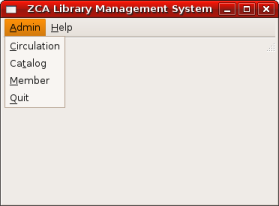
\includegraphics{mainwindow.png}}

В приложении создано специальное окно для управления читателями.  При помощи этого окна реализуются функции \emph{добавление}, \emph{обновление} данных читателя и \emph{удаление} читателя:

\noindent\makebox[\textwidth][c]{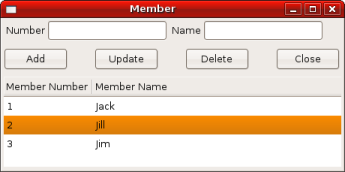
\includegraphics{memberwindow.png}}

Аналогично предыдущему окну, интерфейс управления базой данных книг позволяет \emph{добавлять}, \emph{редактировать} данные и \emph{удалять} книги:

\noindent\makebox[\textwidth][c]{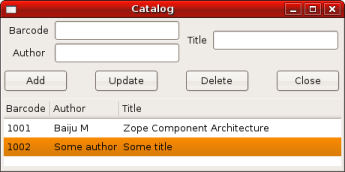
\includegraphics{catalogwindow.png}}

Окно управления книжным фондом реализует функции \emph{выдачи} и \emph{возврата} книг читателями:

\noindent\makebox[\textwidth][c]{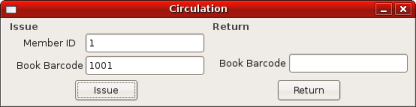
\includegraphics{circulationwindow.png}}


\section{Обзор кода PyGTK%
  \label{pygtk}%
}

Почти все приложение~-- это программный код, использующий PyGTK. Структура программ реализации всех окон схожа, общий вид окон и приложения разработан при помощи дизайнера оконных интерфейсов Glade GUI builder.  Чтобы использовать разработанный интерфейс в программном коде необходимо основным элементам управления поименовать.  В главном меню все пункты поименованы следующим образом: \textquotedbl{}circulation\textquotedbl{}, \textquotedbl{}catalog\textquotedbl{}, \textquotedbl{}member\textquotedbl{}, \textquotedbl{}quit\textquotedbl{} и \textquotedbl{}about\textquotedbl{}.

Класс \texttt{gtk.glade.XML} используется для трансляции и интерпретации файлов glade, в результате его деятельности создаются элементы управления интерфейса пользователя.  Вот пример трансляции и получения доступа к элементу управления:

\begin{minted}{python}
import gtk.glade
xmlobj = gtk.glade.XML('/path/to/file.glade')
widget = xmlobj.get_widget('widget_name')
\end{minted}

В модуле mainwindow.py находится код, аналогичный следующему:

\begin{minted}{python}
curdir = os.path.abspath(os.path.dirname(__file__))
xml = os.path.join(curdir, 'glade', 'mainwindow.glade')
xmlobj = gtk.glade.XML(xml)

self.mainwindow = xmlobj.get_widget('mainwindow')
\end{minted}

Название элемента управления, соответствующего главному окну,~-- \DUroletitlereference{mainwindow}.  Аналогичным образом можно получать доступ и к другим элементам управления.

\begin{minted}{python}
circulation = xmlobj.get_widget('circulation')
member = xmlobj.get_widget('member')
quit = xmlobj.get_widget('quit')
catalog = xmlobj.get_widget('catalog')
about = xmlobj.get_widget('about')
\end{minted}

Затем с элементами управления связываются обработчики возникающих событий.

\begin{minted}{python}
self.mainwindow.connect('delete_event', self.delete_event)
quit.connect('activate', self.delete_event)
circulation.connect('activate', self.on_circulation_activate)
member.connect('activate', self.on_member_activate)
catalog.connect('activate', self.on_catalog_activate)
about.connect('activate', self.on_about_activate)
\end{minted}

Событие \DUroletitlereference{delete\_event} возникает, когда пользователь пытается закрыть окно при помощи соответствующей кнопки.  Событие \DUroletitlereference{activate} инициируется, когда пользователь выбрал какой"=либо пункт меню.  В качестве обработчиков событий выступают функции, вызываемые в момент возникновения события.

В приведенном фрагменте кода видно, что событие \DUroletitlereference{delete\_event} главного окна соединено с методом \DUroletitlereference{on\_delete\_event}.  Событие \DUroletitlereference{activate} элемента \DUroletitlereference{quit} также соединено с этим же методом.

\begin{minted}{python}
def on_delete_event(self, *args):
    gtk.main_quit()
\end{minted}

Функция \DUroletitlereference{on\_delete\_event} просто вызывает функцию \DUroletitlereference{main\_quit}.


\section{Исходный код приложения%
  \label{id52}%
}

Модуль \DUroletitlereference{zcalib.py}:

\begin{minted}{python}
import registry
import mainwindow

if __name__ == '__main__':
    registry.initialize()
    try:
        mainwindow.main()
    except KeyboardInterrupt:
        import sys
        sys.exit(1)
\end{minted}

В тексте импортируются модули \DUroletitlereference{registry} и \DUroletitlereference{mainwindow}.  Затем модуль \DUroletitlereference{registry} инициализируется и вызывается функция \DUroletitlereference{main} модуля \DUroletitlereference{mainwindow}.  Если пользователь попытается завершить программу при помощи комбинации клавиш \DUroletitlereference{Ctrl+C}, программа закончит свое исполнение.  Чтобы заблокировать такое поведение программы, перехватим исключение \DUroletitlereference{KeyboardInterrupt}.

Модуль \DUroletitlereference{registry.py}:

\begin{minted}{python}
import sys
from zope.component import getGlobalSiteManager

from interfaces import IMember
from interfaces import IBook
from interfaces import ICirculation
from interfaces import IDbOperation


def initialize_rdb():
    from interfaces import IRelationalDatabase
    from relationaldatabase import RelationalDatabase
    from member import MemberRDbOperation
    from catalog import BookRDbOperation
    from circulation import CirculationRDbOperation

    gsm = getGlobalSiteManager()
    db = RelationalDatabase()
    gsm.registerUtility(db, IRelationalDatabase)

    gsm.registerAdapter(MemberRDbOperation,
                        (IMember,),
                        IDbOperation)

    gsm.registerAdapter(BookRDbOperation,
                        (IBook,),
                        IDbOperation)

    gsm.registerAdapter(CirculationRDbOperation,
                        (ICirculation,),
                        IDbOperation)

def initialize_odb():
    from interfaces import IObjectDatabase
    from objectdatabase import ObjectDatabase
    from member import MemberODbOperation
    from catalog import BookODbOperation
    from circulation import CirculationODbOperation

    gsm = getGlobalSiteManager()
    db = ObjectDatabase()
    gsm.registerUtility(db, IObjectDatabase)

    gsm.registerAdapter(MemberODbOperation,
                        (IMember,),
                        IDbOperation)

    gsm.registerAdapter(BookODbOperation,
                        (IBook,),
                        IDbOperation)

    gsm.registerAdapter(CirculationODbOperation,
                        (ICirculation,),
                        IDbOperation)

def check_use_relational_db():
    use_rdb = False
    try:
        arg = sys.argv[1]
        if arg == '-r':
            return True
    except IndexError:
        pass
    return use_rdb

def initialize():
    use_rdb = check_use_relational_db()
    if use_rdb:
        initialize_rdb()
    else:
        initialize_odb()
\end{minted}

Обратите внимание на функцию \DUroletitlereference{initialize}, которая вызывается в главном модуле \DUroletitlereference{zcalib.py}.  Функция сначала узнает, какую базу данных надо использовать: реляционную (RDB) или объектную (ODB).  Указание варианта базы данных осуществляется при помощи функции \DUroletitlereference{check\_use\_relational\_db}.  Если в командной строке задать опцию \DUroletitlereference{-r}, будет запущена \DUroletitlereference{initialize\_rdb}, иначе~-- \DUroletitlereference{initialize\_odb}.  Если выбрана RDB, то будут установлены компоненты, реализующие механизм RDB.~В обратном случае~-- компоненты для ODB.

Модуль \DUroletitlereference{mainwindow.py}:

\begin{minted}{python}
import os
import gtk
import gtk.glade

from circulationwindow import circulationwindow
from catalogwindow import catalogwindow
from memberwindow import memberwindow

class MainWindow(object):

    def __init__(self):
        curdir = os.path.abspath(os.path.dirname(__file__))
        xml = os.path.join(curdir, 'glade', 'mainwindow.glade')
        xmlobj = gtk.glade.XML(xml)

        self.mainwindow = xmlobj.get_widget('mainwindow')
        circulation = xmlobj.get_widget('circulation')
        member = xmlobj.get_widget('member')
        quit = xmlobj.get_widget('quit')
        catalog = xmlobj.get_widget('catalog')
        about = xmlobj.get_widget('about')

        self.mainwindow.connect('delete_event', self.delete_event)
        quit.connect('activate', self.delete_event)

        circulation.connect('activate', self.on_circulation_activate)
        member.connect('activate', self.on_member_activate)
        catalog.connect('activate', self.on_catalog_activate)
        about.connect('activate', self.on_about_activate)

    def delete_event(self, *args):
        gtk.main_quit()

    def on_circulation_activate(self, *args):
        circulationwindow.show_all()

    def on_member_activate(self, *args):
        memberwindow.show_all()

    def on_catalog_activate(self, *args):
        catalogwindow.show_all()

    def on_about_activate(self, *args):
        pass

    def run(self):
        self.mainwindow.show_all()

def main():
    mainwindow = MainWindow()
    mainwindow.run()
    gtk.main()
\end{minted}

Функция \DUroletitlereference{main} создает экземпляр класса \DUroletitlereference{MainWindow}, который инициализирует все элементы управления.

Модуль \DUroletitlereference{memberwindow.py}:

\begin{minted}{python}
import os
import gtk
import gtk.glade

from zope.component import getAdapter

from components import Member
from interfaces import IDbOperation


class MemberWindow(object):

    def __init__(self):
        curdir = os.path.abspath(os.path.dirname(__file__))
        xml = os.path.join(curdir, 'glade', 'memberwindow.glade')
        xmlobj = gtk.glade.XML(xml)

        self.memberwindow = xmlobj.get_widget('memberwindow')
        self.number = xmlobj.get_widget('number')
        self.name = xmlobj.get_widget('name')
        add = xmlobj.get_widget('add')
        update = xmlobj.get_widget('update')
        delete = xmlobj.get_widget('delete')
        close = xmlobj.get_widget('close')
        self.treeview = xmlobj.get_widget('treeview')

        self.memberwindow.connect('delete_event', self.on_delete_event)
        add.connect('clicked', self.on_add_clicked)
        update.connect('clicked', self.on_update_clicked)
        delete.connect('clicked', self.on_delete_clicked)
        close.connect('clicked', self.on_delete_event)

        self.initialize_list()

    def show_all(self):
        self.populate_list_store()
        self.memberwindow.show_all()

    def populate_list_store(self):
        self.list_store.clear()
        member = Member()
        memberdboperation = getAdapter(member, IDbOperation)
        members = memberdboperation.get()
        for member in members:
            number = member.number
            name = member.name
            self.list_store.append((member, number, name,))

    def on_delete_event(self, *args):
        self.memberwindow.hide()
        return True

    def initialize_list(self):
        self.list_store = gtk.ListStore(object, str, str)
        self.treeview.set_model(self.list_store)
        tvcolumn = gtk.TreeViewColumn('Member Number')
        self.treeview.append_column(tvcolumn)

        cell = gtk.CellRendererText()
        tvcolumn.pack_start(cell, True)
        tvcolumn.add_attribute(cell, 'text', 1)

        tvcolumn = gtk.TreeViewColumn('Member Name')
        self.treeview.append_column(tvcolumn)

        cell = gtk.CellRendererText()
        tvcolumn.pack_start(cell, True)
        tvcolumn.add_attribute(cell, 'text', 2)

    def on_add_clicked(self, *args):
        number = self.number.get_text()
        name = self.name.get_text()
        member = Member()
        member.number = number
        member.name = name
        self.add(member)
        self.list_store.append((member, number, name,))

    def add(self, member):
        memberdboperation = getAdapter(member, IDbOperation)
        memberdboperation.add()

    def on_update_clicked(self, *args):
        number = self.number.get_text()
        name = self.name.get_text()
        treeselection = self.treeview.get_selection()
        model, iter = treeselection.get_selected()
        if not iter:
            return
        member = self.list_store.get_value(iter, 0)
        member.number = number
        member.name = name
        self.update(member)
        self.list_store.set(iter, 1, number, 2, name)

    def update(self, member):
        memberdboperation = getAdapter(member, IDbOperation)
        memberdboperation.update()

    def on_delete_clicked(self, *args):
        treeselection = self.treeview.get_selection()
        model, iter = treeselection.get_selected()
        if not iter:
            return
        member = self.list_store.get_value(iter, 0)
        self.delete(member)
        self.list_store.remove(iter)

    def delete(self, member):
        memberdboperation = getAdapter(member, IDbOperation)
        memberdboperation.delete()

memberwindow = MemberWindow()
\end{minted}

Модуль \DUroletitlereference{components.py}:

\begin{minted}{python}
from zope.interface import implements

from interfaces import IBook
from interfaces import IMember
from interfaces import ICirculation

class Book(object):

    implements(IBook)

    barcode = ""
    title = ""
    author = ""

class Member(object):

    implements(IMember)

    number = ""
    name = ""

class Circulation(object):

    implements(ICirculation)

    book = Book()
    member = Member()
\end{minted}

Модуль \DUroletitlereference{interfaces.py}:

\begin{minted}{python}
from zope.interface import Interface
from zope.interface import Attribute


class IBook(Interface):

    barcode = Attribute("Barcode")
    author = Attribute("Author of book")
    title = Attribute("Title of book")


class IMember(Interface):

    number = Attribute("ID number")
    name = Attribute("Name of member")


class ICirculation(Interface):

    book = Attribute("A book")
    member = Attribute("A member")


class IRelationalDatabase(Interface):

    def commit():
        pass

    def rollback():
        pass

    def cursor():
        pass

    def get_next_id():
        pass


class IObjectDatabase(Interface):

    def commit():
        pass

    def rollback():
        pass

    def container():
        pass

    def get_next_id():
        pass


class IDbOperation(Interface):

    def get():
        pass

    def add():
        pass

    def update():
        pass

    def delete():
        pass
\end{minted}

Модуль \DUroletitlereference{member.py}:

\begin{minted}{python}
from zope.interface import implements
from zope.component import getUtility
from zope.component import adapts

from components import Member

from interfaces import IRelationalDatabase
from interfaces import IObjectDatabase
from interfaces import IMember
from interfaces import IDbOperation


class MemberRDbOperation(object):

    implements(IDbOperation)
    adapts(IMember)

    def __init__(self, member):
        self.member = member

    def get(self):
        db = getUtility(IRelationalDatabase)
        cr = db.cursor()
        number = self.member.number
        if number:
            cr.execute("""SELECT
                            id,
                            number,
                            name
                          FROM members
                          WHERE number = ?""",
                       (number,))
        else:
            cr.execute("""SELECT
                            id,
                            number,
                            name
                          FROM members""")
        rst = cr.fetchall()
        cr.close()
        members = []
        for record in rst:
            id = record['id']
            number = record['number']
            name = record['name']
            member = Member()
            member.id = id
            member.number = number
            member.name = name
            members.append(member)
        return members

    def add(self):
        db = getUtility(IRelationalDatabase)
        cr = db.cursor()
        next_id = db.get_next_id("members")
        number = self.member.number
        name = self.member.name
        cr.execute("""INSERT INTO members
                        (id, number, name)
                      VALUES (?, ?, ?)""",
                   (next_id, number, name))
        cr.close()
        db.commit()
        self.member.id = next_id

    def update(self):
        db = getUtility(IRelationalDatabase)
        cr = db.cursor()
        number = self.member.number
        name = self.member.name
        id = self.member.id
        cr.execute("""UPDATE members
                        SET
                           number = ?,
                           name = ?
                      WHERE id = ?""",
                   (number, name, id))
        cr.close()
        db.commit()

    def delete(self):
        db = getUtility(IRelationalDatabase)
        cr = db.cursor()
        id = self.member.id
        cr.execute("""DELETE FROM members
                      WHERE id = ?""",
                   (id,))
        cr.close()
        db.commit()


class MemberODbOperation(object):

    implements(IDbOperation)
    adapts(IMember)

    def __init__(self, member):
        self.member = member

    def get(self):
        db = getUtility(IObjectDatabase)
        zcalibdb = db.container()
        members = zcalibdb['members']
        return members.values()

    def add(self):
        db = getUtility(IObjectDatabase)
        zcalibdb = db.container()
        members = zcalibdb['members']
        number = self.member.number
        if number in [x.number for x in members.values()]:
            db.rollback()
            raise Exception("Duplicate key")
        next_id = db.get_next_id('members')
        self.member.id = next_id
        members[next_id] = self.member
        db.commit()

    def update(self):
        db = getUtility(IObjectDatabase)
        zcalibdb = db.container()
        members = zcalibdb['members']
        id = self.member.id
        members[id] = self.member
        db.commit()

    def delete(self):
        db = getUtility(IObjectDatabase)
        zcalibdb = db.container()
        members = zcalibdb['members']
        id = self.member.id
        del members[id]
        db.commit()
\end{minted}


\section{PySQLite%
  \label{pysqlite}%
}


\section{ZODB%
  \label{zodb}%
}

\newpage{}
\section{Заключение%
  \label{id53}%
}

\clearpage
\chapter{Методические указания к выполнению лабораторных работ}
\label{cha:labs}

Чтобы знания, полученные в предыдущих частях учебного пособия, создали почву для формирования навыков использования компонентной архитектуры необходимо выполнить ряд лабораторных работ, которые представлены в разделах данной главы.  Задания на лабораторные работы сформированы таким образом, чтобы следующая лабораторная работа дополняла материал предыдущей.  Это позволяет смотреть на процесс обучения как на маленький проект, состоящий из четырех этапов: разработки компоненты, моделирующей предметную некоторую область или известную структуру данных; создание адаптера интерфейса компоненты из первой лабораторной работы к одной из компонент, представленных в другом варианте задания; разработка оконно интерфейса пользователя, позволяющая вносить изменения в данные компоненты через ее интерфейс; реализация распределенной версии приложения при помощи прокси"=адаптера.

\section{Разработка и тестирование компоненты}
\label{sec:labcomp}
\newpage

\paragraph{Варианты задания}
\newpage

\section{Реализация адаптера интерфейса}
\label{sec:labadapter}
\newpage

\paragraph{Варианты задания}
\newpage

\section{Создание интерфейса пользователя}
\label{sec:labinterface}

\newpage
\paragraph{Варианты задания}
\newpage

\section{Моделирование распределенного приложения}
\label{sec:labmodel}
\newpage

\paragraph{Варианты задания}
\newpage


\chapter{Справочник%
  \label{id54}%
}


\section*{adaptedBy%
  \label{adaptedby}%
}

Функция возвращает перечень интерфейсов, адаптируемых объектом"=адаптером.

\begin{itemize}

\item Модуль: \texttt{zope.component}

\item Сигнатура: \DUroletitlereference{adaptedBy(object)}

\end{itemize}

Пример:

\begin{minted}{python}
    from zope.interface import implements
    from zope.component import adapts
    from zope.component import adaptedBy

    class FrontDeskNG(object):

        implements(IDesk)
        adapts(IGuest)

        def __init__(self, guest):
            self.guest = guest

    adaptedBy(FrontDeskNG)
(<InterfaceClass __builtin__.IGuest>,)
\end{minted}


\section*{adapter%
  \label{id55}%
}

Адаптерами выступают любые вызываемые (callable) объекты.  Также существует специальный декоратор \DUroletitlereference{adapter}, который позволяет декларировать вызываемые объекты как адаптеры для указанных интерфейсов (или классов).

\begin{itemize}

\item Модуль: \texttt{zope.component}

\item Спецификация: \DUroletitlereference{adapter(*interfaces)}

\end{itemize}

Пример:

\begin{minted}{python}
    from zope.interface import Attribute
    from zope.interface import Interface
    from zope.interface import implementer
    from zope.component import adapter
    from zope.interface import implements

    class IJob(Interface):
        """A job"""

    class Job(object):
        implements(IJob)

    class IPerson(Interface):

        name = Attribute("Name")
        job = Attribute("Job")

    class Person(object):
        implements(IPerson)

        name = None
        job = None

    @implementer(IJob)
    @adapter(IPerson)
    def personJob(person):
        return person.job

    jack = Person()
    jack.name = "Jack"
    jack.job = Job()
    personJob(jack)
<Job object at ...>
\end{minted}


\section*{adapts%
  \label{adapts}%
}

Функция определяющая, что некоторый класс является адаптером.

\begin{itemize}

\item Модуль: \texttt{zope.component}

\item Спецификация: \DUroletitlereference{adapts(*interfaces)}

\end{itemize}

Пример:

\begin{minted}{python}
    from zope.interface import implements
    from zope.component import adapts

    class FrontDeskNG(object):

        implements(IDesk)
        adapts(IGuest)

        def __init__(self, guest):
            self.guest = guest

        def register(self):
            next_id = get_next_id()
            bookings_db[next_id] = {
            'name': guest.name,
            'place': guest.place,
            'phone': guest.phone
            }
\end{minted}


\section*{alsoProvides%
  \label{alsoprovides}%
}

Задает объекту перечень интерфейсов, которые он обслуживать, в дополнение к ранее декларированным.  Параметры функции, следующие за объектом,~-- перечень обслуживаемых интерфейсов (один или несколько).

\begin{itemize}

\item Модуль: \texttt{zope.interface}

\item Спецификация: \DUroletitlereference{alsoProvides(object, *interfaces)}

\end{itemize}

Пример:

\begin{minted}{python}
    from zope.interface import Attribute
    from zope.interface import Interface
    from zope.interface import implements
    from zope.interface import alsoProvides

    class IPerson(Interface):

        name = Attribute("Name of person")

    class IStudent(Interface):

        college = Attribute("Name of college")

    class Person(object):

        implements(IDesk)
        name = u""

    jack = Person()
    jack.name = "Jack"
    jack.college = "New College"
    alsoProvides(jack, IStudent)

You can test it like this:

    from zope.interface import providedBy
    IStudent in providedBy(jack)
True
\end{minted}


\section*{Attribute%
  \label{attribute}%
}

Класс, предназначенный для определения атрибутов в интерфейсе.

\begin{itemize}

\item Модуль: \texttt{zope.interface}

\item Спецификация: \DUroletitlereference{Attribute(name, doc='')}

\item Смотри также: \hyperref[interface]{Interface}

\end{itemize}

Пример:

\begin{minted}{python}
    from zope.interface import Attribute
    from zope.interface import Interface

    class IPerson(Interface):

        name = Attribute("Name of person")
        email = Attribute("Email Address")
\end{minted}


\section*{classImplements%
  \label{classimplements}%
}

Задает дополнительные интерфейсы классу, которые он в системе будет реализовывать.  Перечень аргументов, следующих за классом~-- задаваемые интерфейсы, которые добавляются к списку ранее заданных интерфейсов.

\begin{itemize}

\item Модуль: \texttt{zope.interface}

\item Спецификация: \DUroletitlereference{classImplements(cls, *interfaces)}

\end{itemize}

Пример:

\begin{minted}{python}
    from zope.interface import Attribute
    from zope.interface import Interface
    from zope.interface import implements
    from zope.interface import classImplements

    class IPerson(Interface):

        name = Attribute("Имя человека")

    class IStudent(IPerson):

        college = Attribute("Название колледжа")

    class Person(object):

        implements(IDesk)
        name = u""
        college = u""

    classImplements(Person, IStudent)
    ganes = Person()
    ganes.name = "Баролби Гейнс"
    ganes.college = "Саус-хермондский институт технологий"

Результат тестируется следующим образом:

    from zope.interface import providedBy
    IStudent in providedBy(ganes)
True
\end{minted}


\section*{classImplementsOnly%
  \label{classimplementsonly}%
}

Задает классу набор реализуемых им интерфейсов.  Перечень аргументов после класса~-- задаваемые интерфейсы.  Ранее декларированные интерфейсы заменяются данным перечнем.

\begin{quote}

\begin{itemize}

\item Модуль: \texttt{zope.interface}

\item Спецификация: \DUroletitlereference{classImplementsOnly(cls, *interfaces)}

\end{itemize}

\end{quote}

Пример:

\begin{minted}{python}
    from zope.interface import Attribute
    from zope.interface import Interface
    from zope.interface import implements
    from zope.interface import classImplementsOnly

    class IPerson(Interface):

        name = Attribute("Name of person")

    class IStudent(Interface):

        college = Attribute("Name of college")

    class Person(object):

        implements(IPerson)
        college = u""

    classImplementsOnly(Person, IStudent)
    jack = Person()
    jack.college = "New College"

Результат тестируется следующим образом:

    from zope.interface import providedBy
    IPerson in providedBy(jack)
False
    IStudent in providedBy(jack)
True
\end{minted}


\section*{classProvides%
  \label{classprovides}%
}

Обычно если класс реализует определенный интерфейс, то его экземпляры обслуживают этот интерфейс.  Но когда надо, чтобы именно класс обслуживал некоторый интерфейс, то это реализуется функцией \texttt{classProvides}.

\begin{itemize}

\item Модуль: \texttt{zope.interface}

\item Спецификация: \DUroletitlereference{classProvides(*interfaces)}

\end{itemize}

Пример:

\begin{minted}{python}
    from zope.interface import Attribute
    from zope.interface import Interface
    from zope.interface import classProvides

    class IPerson(Interface):

        name = Attribute("Name of person")

    class Person(object):

        classProvides(IPerson)
        name = u"Jack"

Результат тестируется следующим образом:

    from zope.interface import providedBy
    IPerson in providedBy(Person)
True
\end{minted}


\section*{ComponentLookupError%
  \label{componentlookuperror}%
}

Исключение, которое инициируется, если поиск компоненты не удался.

Пример:

\begin{minted}{python}
    class IPerson(Interface):

        name = Attribute("Name of person")

    person = object()
    getAdapter(person, IPerson, 'not-exists')
Traceback (most recent call last):

ComponentLookupError: ...
\end{minted}


\section*{createObject%
  \label{createobject}%
}

Создает объект, используя фабрику.

Производит поиск поименованной фабрики в текущем регистре компонент (менеджере сайта) и запускает ее с заданными аргументами.  Если такой фабрики не удается найти, инициируется исключение \texttt{ComponentLookupError}.  Возвращает созданный объект.

При помощи ключевого слова \DUroletitlereference{context} в аргументе функции задается контекст, где следует искать фабрику, в отличие от основного регистра.  Ограничения технологии не позволяют передавать аргумент по ключу \textquotedbl{}context\textquotedbl{} в фабрику.

\begin{itemize}

\item Модуль: \texttt{zope.component}

\item Спецификация: \DUroletitlereference{createObject(factory\_name, *args, **kwargs)}

\end{itemize}

Пример:

\begin{minted}{python}
    from zope.interface import Attribute
    from zope.interface import Interface
    from zope.interface import implements

    class IDatabase(Interface):

        def getConnection():
            """Return connection object"""

    class FakeDb(object):

        implements(IDatabase)

        def getConnection(self):
            return "connection"

    from zope.component.factory import Factory

    factory = Factory(FakeDb, 'FakeDb')

    from zope.component import getGlobalSiteManager
    gsm = getGlobalSiteManager()

    from zope.component.interfaces import IFactory
    gsm.registerUtility(factory, IFactory, 'fakedb')

    from zope.component import createObject
    createObject('fakedb')
<FakeDb object at ...>
\end{minted}


\section*{Declaration%
  \label{declaration}%
}

Непосредственно не запускается.


\section*{directlyProvidedBy%
  \label{directlyprovidedby}%
}

Возвращает список интерфейсов, которые непосредственно обслуживаются объектом, переданным в параметре.

\begin{itemize}

\item Модуль: \texttt{zope.interface}

\item Спецификация: \DUroletitlereference{directlyProvidedBy(object)}

\end{itemize}

Пример:

\begin{minted}{python}
    from zope.interface import Attribute
    from zope.interface import Interface

    class IPerson(Interface):

        name = Attribute("Name of person")

    class IStudent(Interface):

        college = Attribute("Name of college")

    class ISmartPerson(Interface):
        pass

    class Person(object):

        implements(IPerson)
        name = u""

    jack = Person()
    jack.name = u"Jack"
    jack.college = "New College"
    alsoProvides(jack, ISmartPerson, IStudent)

    from zope.interface import directlyProvidedBy

    jack_dp = directlyProvidedBy(jack)
    IPerson in jack_dp.interfaces()
False
    IStudent in jack_dp.interfaces()
True
    ISmartPerson in jack_dp.interfaces()
True
\end{minted}


\section*{directlyProvides%
  \label{directlyprovides}%
}

Задает перечень интерфейсов, обслуживаемых объектом.  Аргументы, непосредственно следующие за объектом~-- перечень декларируемых интерфейсов.  Заданные интерфейсы заменяют декларированные ранее.

\begin{quote}

\begin{itemize}

\item Модуль: \texttt{zope.interface}

\item Спецификация: \DUroletitlereference{directlyProvides(object, *interfaces)}

\end{itemize}

\end{quote}

Пример:

\begin{minted}{python}
    from zope.interface import Attribute
    from zope.interface import Interface

    class IPerson(Interface):

        name = Attribute("Name of person")

    class IStudent(Interface):

        college = Attribute("Name of college")

    class ISmartPerson(Interface):
        pass

    class Person(object):

        implements(IPerson)
        name = u""

    jack = Person()
    jack.name = u"Jack"
    jack.college = "New College"
    alsoProvides(jack, ISmartPerson, IStudent)

    from zope.interface import directlyProvidedBy

    jack_dp = directlyProvidedBy(jack)
    ISmartPerson in jack_dp.interfaces()
True
    IPerson in jack_dp.interfaces()
False
    IStudent in jack_dp.interfaces()
True
    from zope.interface import providedBy

    ISmartPerson in providedBy(jack)
True

    from zope.interface import directlyProvides
    directlyProvides(jack, IStudent)

    jack_dp = directlyProvidedBy(jack)
    ISmartPerson in jack_dp.interfaces()
False
    IPerson in jack_dp.interfaces()
False
    IStudent in jack_dp.interfaces()
True

    ISmartPerson in providedBy(jack)
False
\end{minted}


\section*{getAdapter%
  \label{getadapter}%
}

Возвращает поименованный адаптер к заданному интерфейсу для заданного объекта.  Если подходящего адаптера не получается найти, создается исключительная ситуация \texttt{ComponentLookupError}.

\begin{itemize}

\item Модуль: \texttt{zope.interface}

\item Спецификация: \DUroletitlereference{getAdapter(object, interface=Interface, name=u'', context=None)}

\end{itemize}

Пример:

\begin{minted}{python}
    from zope.interface import Attribute
    from zope.interface import Interface

    class IDesk(Interface):
        """A frontdesk will register object's details"""

        def register():
            """Register object's details"""


    from zope.interface import implements
    from zope.component import adapts

    class FrontDeskNG(object):

        implements(IDesk)
        adapts(IGuest)

        def __init__(self, guest):
            self.guest = guest

        def register(self):
            next_id = get_next_id()
            bookings_db[next_id] = {
            'name': guest.name,
            'place': guest.place,
            'phone': guest.phone
            }

    class Guest(object):

        implements(IGuest)

        def __init__(self, name, place):
            self.name = name
            self.place = place

    jack = Guest("Jack", "Bangalore")
    jack_frontdesk = FrontDeskNG(jack)

    IDesk.providedBy(jack_frontdesk)
True

    from zope.component import getGlobalSiteManager
    gsm = getGlobalSiteManager()
    gsm.registerAdapter(FrontDeskNG,
                        (IGuest,), IDesk, 'ng')

    getAdapter(jack, IDesk, 'ng')
<FrontDeskNG object at ...>
\end{minted}


\section*{getAdapterInContext%
  \label{getadapterincontext}%
}

Вместо этой функции следует использовать аргумент \DUroletitlereference{context} функции \hyperref[getadapter]{getAdapter}.

\begin{itemize}

\item Модуль: \texttt{zope.component}

\item Спецификация: \DUroletitlereference{getAdapterInContext(object, interface, context)}

\item Смотри также: \hyperref[queryadapterincontext]{queryAdapterInContext}

\end{itemize}

Пример:

\begin{minted}{python}
    from zope.component.globalregistry import BaseGlobalComponents
    from zope.component import IComponentLookup
    sm = BaseGlobalComponents()

    class Context(object):
        def __init__(self, sm):
            self.sm = sm
        def __conform__(self, interface):
            if interface.isOrExtends(IComponentLookup):
                return self.sm

    context = Context(sm)

    from zope.interface import Attribute
    from zope.interface import Interface

    class IDesk(Interface):
        """A frontdesk will register object's details"""

        def register():
            """Register object's details"""


    from zope.interface import implements
    from zope.component import adapts

    class FrontDeskNG(object):

        implements(IDesk)
        adapts(IGuest)

        def __init__(self, guest):
            self.guest = guest

        def register(self):
            next_id = get_next_id()
            bookings_db[next_id] = {
            'name': guest.name,
            'place': guest.place,
            'phone': guest.phone
            }

    class Guest(object):

        implements(IGuest)

        def __init__(self, name, place):
            self.name = name
            self.place = place

    jack = Guest("Jack", "Bangalore")
    jack_frontdesk = FrontDeskNG(jack)

    IDesk.providedBy(jack_frontdesk)
True

    from zope.component import getGlobalSiteManager
    gsm = getGlobalSiteManager()
    sm.registerAdapter(FrontDeskNG,
                        (IGuest,), IDesk)

    from zope.component import getAdapterInContext

    getAdapterInContext(jack, IDesk, sm)
<FrontDeskNG object at ...>
\end{minted}


\section*{getAdapters%
  \label{getadapters}%
}

Осуществляет поиск всех подходящих адаптеров к заданному интерфейсу и заданным объектам.  Возвращает список адаптеров.  Если в списке есть поименованный адаптер, то выдается наиболее специфический адаптер с заданным именем.

\begin{itemize}

\item Модуль: \texttt{zope.component}

\item Спецификация: \DUroletitlereference{getAdapters(objects, provided, context=None)}

\end{itemize}

Пример:

\begin{minted}{python}
    from zope.interface import implements
    from zope.component import adapts

    class FrontDeskNG(object):

        implements(IDesk)
        adapts(IGuest)

        def __init__(self, guest):
            self.guest = guest

        def register(self):
            next_id = get_next_id()
            bookings_db[next_id] = {
            'name': guest.name,
            'place': guest.place,
            'phone': guest.phone
            }

    jack = Guest("Jack", "Bangalore")
    jack_frontdesk = FrontDeskNG(jack)

    from zope.component import getGlobalSiteManager
    gsm = getGlobalSiteManager()

    gsm.registerAdapter(FrontDeskNG, name='ng')

    from zope.component import getAdapters
    list(getAdapters((jack,), IDesk))
[(u'ng', <FrontDeskNG object at ...>)]
\end{minted}


\section*{getAllUtilitiesRegisteredFor%
  \label{getallutilitiesregisteredfor}%
}

Возвращает все зарегистрированные утилиты для заданного интерфейса, в том числе и те, которые были заменены (overridden).  По возвращаемому значению можно осуществлять итерацию, где каждый элемент~-- это утилита.

\begin{itemize}

\item Модуль: \texttt{zope.component}

\item Спецификация: \DUroletitlereference{getAllUtilitiesRegisteredFor(interface)}

\end{itemize}

Пример:

\begin{minted}{python}
    from zope.interface import Interface
    from zope.interface import implements

    class IGreeter(Interface):
        def greet(name):
            "say hello"

    class Greeter(object):

        implements(IGreeter)

        def greet(self, name):
            print "Hello", name

    from zope.component import getGlobalSiteManager
    gsm = getGlobalSiteManager()

    greet = Greeter()
    gsm.registerUtility(greet, IGreeter)

    from zope.component import getAllUtilitiesRegisteredFor

    getAllUtilitiesRegisteredFor(IGreeter)
[<Greeter object at ...>]
\end{minted}


\section*{getFactoriesFor%
  \label{getfactoriesfor}%
}

Возвращает список двоек (name, factory) зарегистрированных фабрик классов, реализующих заданный интерфейс.

\begin{quote}

\begin{itemize}

\item Модуль: \texttt{zope.component}

\item Спецификация: \DUroletitlereference{getFactoriesFor(interface, context=None)}

\end{itemize}

\end{quote}

Пример:

\begin{minted}{python}
    from zope.interface import Attribute
    from zope.interface import Interface
    from zope.interface import implements

    class IDatabase(Interface):

        def getConnection():
            """Return connection object"""

    class FakeDb(object):

        implements(IDatabase)

        def getConnection(self):
            return "connection"

    from zope.component.factory import Factory

    factory = Factory(FakeDb, 'FakeDb')

    from zope.component import getGlobalSiteManager
    gsm = getGlobalSiteManager()

    from zope.component.interfaces import IFactory
    gsm.registerUtility(factory, IFactory, 'fakedb')

    from zope.component import getFactoriesFor

    list(getFactoriesFor(IDatabase))
[(u'fakedb', <Factory for <class 'FakeDb'>{}>)]
\end{minted}


\section*{getFactoryInterfaces%
  \label{getfactoryinterfaces}%
}

Возвращает перечень интерфейсов, реализуемых фабрикой.  Производит поиск по заданному имени фабрики, которая находится в ближайшем контексте, затем возвращает либо ее интерфейс, либо n"=ку (tuple) интерфейсов, которые будут обслуживать объекты, создаваемые данной фабрикой.

\begin{itemize}

\item Модуль: \texttt{zope.component}

\item Спецификация: \DUroletitlereference{getFactoryInterfaces(name, context=None)}

\end{itemize}

Пример:

\begin{minted}{python}
    from zope.interface import Attribute
    from zope.interface import Interface
    from zope.interface import implements

    class IDatabase(Interface):

        def getConnection():
            """Return connection object"""

    class FakeDb(object):

        implements(IDatabase)

        def getConnection(self):
            return "connection"

    from zope.component.factory import Factory

    factory = Factory(FakeDb, 'FakeDb')

    from zope.component import getGlobalSiteManager
    gsm = getGlobalSiteManager()

    from zope.component.interfaces import IFactory
    gsm.registerUtility(factory, IFactory, 'fakedb')

    from zope.component import getFactoryInterfaces

    getFactoryInterfaces('fakedb')
<implementedBy __builtin__.FakeDb>
\end{minted}


\section*{getGlobalSiteManager%
  \label{getglobalsitemanager}%
}

Функция возвращает глобальный регистр компонент (глобальный менеджер сайта).  Эта функция всегда должна успешно выполнится.  Возвращаемый регистр обслуживает интерфейс \DUroletitlereference{IGlobalSiteManager}.

\begin{itemize}

\item Модуль: \texttt{zope.component}

\item Спецификация: \DUroletitlereference{getGlobalSiteManager()}

\end{itemize}

Пример:

\begin{minted}{python}
    from zope.component import getGlobalSiteManager
    from zope.component import globalSiteManager
    gsm = getGlobalSiteManager()
    gsm is globalSiteManager
True
\end{minted}


\section*{getMultiAdapter%
  \label{getmultiadapter}%
}

Осуществляет поиск мультиадаптера (multi"=adapter) к заданному интерфейсу и набору адаптируемых объектов.  Возвращает мультиадаптер, который способен адаптировать эти объекты к указанному интерфейсу.  Если такого адаптера найти не удается, то создается исключение \DUroletitlereference{ComponentLookupError}.  Пустое имя адаптера зарезервировано для непоименнованных адаптеров.  Функции, реализующие поиск непоименнованных адаптеров,~-- это функции поиска адаптеров, где в качестве имени адаптера задается пустая строка.

\begin{itemize}

\item Модуль: \texttt{zope.component}

\item Спецификация: \DUroletitlereference{getMultiAdapter(objects, interface=Interface, name='', context=None)}

\item Смотри также: \hyperref[querymultiadapter]{queryMultiAdapter}

\end{itemize}

Пример:

\begin{minted}{python}
    from zope.interface import Interface
    from zope.interface import implements
    from zope.component import adapts

    class IAdapteeOne(Interface):
        pass

    class IAdapteeTwo(Interface):
        pass

    class IFunctionality(Interface):
        pass

    class MyFunctionality(object):
        implements(IFunctionality)
        adapts(IAdapteeOne, IAdapteeTwo)

        def __init__(self, one, two):
            self.one = one
            self.two = two

    from zope.component import getGlobalSiteManager
    gsm = getGlobalSiteManager()

    gsm.registerAdapter(MyFunctionality)

    class One(object):
        implements(IAdapteeOne)

    class Two(object):
        implements(IAdapteeTwo)

    one = One()
    two = Two()

    from zope.component import getMultiAdapter

    getMultiAdapter((one,two), IFunctionality)
<MyFunctionality object at ...>

    myfunctionality = getMultiAdapter((one,two), IFunctionality)
    myfunctionality.one
<One object at ...>
    myfunctionality.two
<Two object at ...>
\end{minted}


\section*{getSiteManager%
  \label{getsitemanager}%
}

Возвращает регистр компонент (менеджер сайта), который является наиближайщем в заданном контексте. Если параметр \DUroletitlereference{context} равен \DUroletitlereference{None}, то возвращается глобальный регистр.  Если параметр \DUroletitlereference{context} не равен \DUroletitlereference{None}, то предполагается, что найдется какой"=либо адаптер из \DUroletitlereference{context}-а \DUroletitlereference{IComponentLookup}.  Если же найти такой адаптер на самом деле не удалось, создается исключение \DUroletitlereference{ComponentLookupError}.

\begin{itemize}

\item Модуль: \texttt{zope.component}

\item Спецификация: \DUroletitlereference{getSiteManager(context=None)}

\end{itemize}

Пример 1:

\begin{minted}{python}
    from zope.component.globalregistry import BaseGlobalComponents
    from zope.component import IComponentLookup
    sm = BaseGlobalComponents()

    class Context(object):
        def __init__(self, sm):
            self.sm = sm
        def __conform__(self, interface):
            if interface.isOrExtends(IComponentLookup):
                return self.sm

    context = Context(sm)

    from zope.component import getSiteManager

    lsm = getSiteManager(context)
    lsm is sm
True
\end{minted}

Пример 2:

\begin{minted}{python}
    from zope.component import getGlobalSiteManager
    gsm = getGlobalSiteManager()

    sm = getSiteManager()
    gsm is sm
True
\end{minted}


\section*{getUtilitiesFor%
  \label{getutilitiesfor}%
}

Осуществляет поиск зарегистрированных утилит, которые оснащают заданный интерфейс.  Возвращает объект, генерирующий двойки (name, utility).

\begin{itemize}

\item Модуль: \texttt{zope.component}

\item Спецификация: \DUroletitlereference{getUtilitiesFor(interface)}

\end{itemize}

Пример:

\begin{minted}{python}
    from zope.interface import Interface
    from zope.interface import implements

    class IGreeter(Interface):
        def greet(name):
            "say hello"

    class Greeter(object):

        implements(IGreeter)

        def greet(self, name):
            print "Hello", name

    from zope.component import getGlobalSiteManager
    gsm = getGlobalSiteManager()

    greet = Greeter()
    gsm.registerUtility(greet, IGreeter)

    from zope.component import getUtilitiesFor

    list(getUtilitiesFor(IGreeter))
[(u'', <Greeter object at ...>)]
\end{minted}


\section*{getUtility%
  \label{getutility}%
}

Возвращает утилиту, которая обслуживает заданный интерфейс.  Возвращает утилиту, которая находится в ближайшем из контекстов.  Если такой утилиты не удается найти, то создается исключение \texttt{ComponentLookupError}.

\begin{itemize}

\item Модуль: \texttt{zope.component}

\item Спецификация: \DUroletitlereference{getUtility(interface, name='', context=None)}

\end{itemize}

Пример:

\begin{minted}{python}
    from zope.interface import Interface
    from zope.interface import implements

    class IGreeter(Interface):
        def greet(name):
            "say hello"

    class Greeter(object):

        implements(IGreeter)

        def greet(self, name):
            return "Hello " + name

    from zope.component import getGlobalSiteManager
    gsm = getGlobalSiteManager()

    greet = Greeter()
    gsm.registerUtility(greet, IGreeter)

    from zope.component import getUtility

    getUtility(IGreeter).greet('Jack')
'Hello~Jack'
\end{minted}


\section*{handle%
  \label{handle}%
}

Запускает все обработчики (handlers) для заданных объектов.  Обработчики~-- это фабрики адаптеров"=подписчиков (subscription adapter), которые ничего не возвращают.  Они просто выполняют некоторую процедуру.  Обработчики обычно используются для реализации реакции на событие.

\begin{itemize}

\item Модуль: \texttt{zope.component}

\item Спецификация: \DUroletitlereference{handle(*objects)}

\end{itemize}

Пример:

\begin{minted}{python}
    import datetime

    def documentCreated(event):
        event.doc.created = datetime.datetime.utcnow()

    from zope.interface import Interface
    from zope.interface import Attribute
    from zope.interface import implements

    class IDocumentCreated(Interface):
        doc = Attribute("The document that was created")

    class DocumentCreated(object):
        implements(IDocumentCreated)

        def __init__(self, doc):
            self.doc = doc


    def documentCreated(event):
        event.doc.created = datetime.datetime.utcnow()

    from zope.component import adapter

    @adapter(IDocumentCreated)
    def documentCreated(event):
        event.doc.created = datetime.datetime.utcnow()


    from zope.component import getGlobalSiteManager
    gsm = getGlobalSiteManager()

    gsm.registerHandler(documentCreated)

    from zope.component import handle

    handle(DocumentCreated(doc))
    doc.created.__class__.__name__
'datetime'
\end{minted}


\section*{implementedBy%
  \label{implementedby}%
}

Возвращает перечень интерфейсов, реализуемых заданным классом.

\begin{itemize}

\item Модуль: \texttt{zope.interface}

\item Спецификация: \DUroletitlereference{implementedBy(class\_)}

\end{itemize}

Пример 1:

\begin{minted}{python}
    from zope.interface import Interface
    from zope.interface import implements

    class IGreeter(Interface):
        def greet(name):
            "say hello"

    class Greeter(object):

        implements(IGreeter)

        def greet(self, name):
            print "Hello", name

    from zope.interface import implementedBy
    implementedBy(Greeter)
<implementedBy __builtin__.Greeter>
\end{minted}

Пример 2:

\begin{minted}{python}
    from zope.interface import Attribute
    from zope.interface import Interface
    from zope.interface import implements

    class IPerson(Interface):
        name = Attribute("Name of person")

    class ISpecial(Interface):
        pass

    class Person(object):
        implements(IPerson)
        name = u""

    from zope.interface import classImplements
    classImplements(Person, ISpecial)

    from zope.interface import implementedBy

To get a list of all interfaces implemented by that class::

    [x.__name__ for x in implementedBy(Person)]
['IPerson', 'ISpecial']
\end{minted}


\section*{implementer%
  \label{implementer}%
}

Создает декоратор (decorator) для задания интерфейса, реализуемого фабрикой.  Возвращает исполняемый объект (callable), которые представляет собой фабрику, обрамляющую объект, переданный декоратору в качестве параметра.

\begin{itemize}

\item Модуль: \texttt{zope.interface}

\item Спецификация: \DUroletitlereference{implementer(*interfaces)}

\end{itemize}

Пример:

\begin{minted}{python}
    from zope.interface import implementer
    class IFoo(Interface):
        pass
    class Foo(object):
        implements(IFoo)

    @implementer(IFoo)
    def foocreator():
        foo = Foo()
        return foo
    list(implementedBy(foocreator))
[<InterfaceClass __builtin__.IFoo>]
\end{minted}


\section*{implements%
  \label{implements}%
}

Функция вызывается внутри определения класса.  Функция задает перечень интерфейсов, которые класс намеревается реализовать.  Реализуемые интерфейсы задаются в качестве параметров функции.  Заданные интерфейсы добавляются ранее декларированным, включая интерфейсы, получаемые при наследовании.  Функция \DUroletitlereference{implementsOnly} используется для задания перечня интерфейсов, при этом унаследованные и ранее декларированные интерфейсы заменяются.

\begin{itemize}

\item Модуль: \texttt{zope.interface}

\item Спецификация: \DUroletitlereference{implements(*interfaces)}

\end{itemize}

Пример:

\begin{minted}{python}
    from zope.interface import Attribute
    from zope.interface import Interface
    from zope.interface import implements

    class IPerson(Interface):

        name = Attribute("Name of person")

    class Person(object):

        implements(IPerson)
        name = u""

    jack = Person()
    jack.name = "Jack"

You can test it like this:

    from zope.interface import providedBy
    IPerson in providedBy(jack)
True
\end{minted}


\section*{implementsOnly%
  \label{implementsonly}%
}

Задает перечень интерфейсов, реализуемых классом, при этом ранее сделанные и унаследованные декларации интерфейсов отменяются (overridden).  Эта функция выполняется в процессе определения класса.  Аргументы функции~-- декларируемые интерфейсы.

\begin{itemize}

\item Модуль: \texttt{zope.interface}

\item Спецификация: \DUroletitlereference{implementsOnly(*interfaces)}

\end{itemize}

Пример:

\begin{minted}{python}
    from zope.interface import Attribute
    from zope.interface import Interface
    from zope.interface import implements
    from zope.interface import implementsOnly

    class IPerson(Interface):

        name = Attribute("Name of person")

    class IStudent(Interface):

        college = Attribute("Name of college")

    class Person(object):

        implements(IPerson)
        name = u""

    class NewPerson(Person):
        implementsOnly(IStudent)
        college = u""

    jack = NewPerson()
    jack.college = "New College"

You can test it like this:

    from zope.interface import providedBy
    IPerson in providedBy(jack)
False
    IStudent in providedBy(jack)
True
\end{minted}


\section*{Interface%
  \label{interface}%
}

При помощи данного класса задаются интерфейсы. Интерфейсы~-- это особые классы Python.  Чтобы определить класс"=интерфейс надо просто унаследовать \texttt{Interface}.

\begin{itemize}

\item Модуль: \texttt{zope.interface}

\item Спецификация: \DUroletitlereference{Interface(name, doc='')}

\end{itemize}

Пример 1:

\begin{minted}{python}
    from zope.interface import Attribute
    from zope.interface import Interface

    class IPerson(Interface):

        name = Attribute("Name of person")
        email = Attribute("Email Address")
\end{minted}

Пример 2:

\begin{minted}{python}
    from zope.interface import Interface

    class IHost(Interface):

        def goodmorning(guest):
            """Say good morning to guest"""
\end{minted}


\section*{moduleProvides%
  \label{moduleprovides}%
}

Определить модуль Python как объект, обслуживающий заданный интерфейс.  Функция используется в тексте определения модуля.  Аргументы~-- один или несколько интерфейсов.  Исключительная ситуация создается в случае, если в модуле уже ранее встречалась такая декларация.  Другими словами, в модуле декларация интерфейсов должна быть только одна.

Функция \DUroletitlereference{moduleProvides}~-- это удобный вариант функции \texttt{directlyProvides}, применяемой к объекту"=модулю.

\begin{itemize}

\item Модуль: \texttt{zope.interface}

\item Спецификация: \DUroletitlereference{moduleProvides(*interfaces)}

\item Смотри также: \hyperref[directlyprovides]{directlyProvides}

\end{itemize}

В исходном коде модуля \DUroletitlereference{zope.component} эта функция применяется, а именно, в файле \DUroletitlereference{\_\_init\_\_.py} есть следующие операторы:

\begin{minted}{python}
moduleProvides(IComponentArchitecture,
               IComponentRegistrationConvenience)
\end{minted}

Таким образом, \DUroletitlereference{zope.component} оснащает два интерфейса: \DUroletitlereference{IComponentArchitecture} и \DUroletitlereference{IComponentRegistrationConvenience}.


\section*{noLongerProvides%
  \label{nolongerprovides}%
}

Исключить заданный интерфейс из списка интерфейсов, обслуживаемых объектом.

\begin{itemize}

\item Модуль: \texttt{zope.interface}

\item Спецификация: \DUroletitlereference{noLongerProvides(object, interface)}

\end{itemize}

Пример:

\begin{minted}{python}
    from zope.interface import Attribute
    from zope.interface import Interface
    from zope.interface import implements
    from zope.interface import classImplements

    class IPerson(Interface):

        name = Attribute("Name of person")

    class IStudent(Interface):

        college = Attribute("Name of college")

    class Person(object):

        implements(IPerson)
        name = u""

    jack = Person()
    jack.name = "Jack"
    jack.college = "New College"
    directlyProvides(jack, IStudent)

You can test it like this:

    from zope.interface import providedBy
    IPerson in providedBy(jack)
True
    IStudent in providedBy(jack)
True
    from zope.interface import noLongerProvides
    noLongerProvides(jack, IStudent)
    IPerson in providedBy(jack)
True
    IStudent in providedBy(jack)
False
\end{minted}


\section*{provideAdapter%
  \label{provideadapter}%
}

Вместо этой функции рекомендовано использовать функцию \hyperref[registeradapter]{registerAdapter} .


\section*{provideHandler%
  \label{providehandler}%
}

Вместо этой функции рекомендовано использовать функцию \hyperref[registerhandler]{registerHandler} .


\section*{provideSubscriptionAdapter%
  \label{providesubscriptionadapter}%
}

Вместо этой функции рекомендовано использовать функцию \hyperref[registersubscriptionadapter]{registerSubscriptionAdapter} .


\section*{provideUtility%
  \label{provideutility}%
}

Вместо этой функции рекомендовано использовать функцию \hyperref[registerutility]{registerUtility} .


\section*{providedBy%
  \label{providedby}%
}

Функция проверят, обслуживает ли объект указанный интерфейс.  Возврящается \DUroletitlereference{истина}, если ZCA допускает, что это так, в том числе, если объект оснащает расширенный интерфейс.

\begin{itemize}

\item Модуль: \texttt{zope.interface}

\item Спецификация: \DUroletitlereference{providedBy(object)}

\end{itemize}

Пример 1:

\begin{minted}{python}
    from zope.interface import Attribute
    from zope.interface import Interface
    from zope.interface import implements

    class IPerson(Interface):

        name = Attribute("Name of person")

    class Person(object):

        implements(IPerson)
        name = u""

    jack = Person()
    jack.name = "Jack"

Результат проверяется следующим образом:

    from zope.interface import providedBy
    IPerson in providedBy(jack)
True
\end{minted}

Пример 2:

\begin{minted}{python}
    from zope.interface import Attribute
    from zope.interface import Interface
    from zope.interface import implements

    class IPerson(Interface):
        name = Attribute("Name of person")

    class ISpecial(Interface):
        pass

    class Person(object):
        implements(IPerson)
        name = u""

    from zope.interface import classImplements
    classImplements(Person, ISpecial)
    from zope.interface import providedBy
    jack = Person()
    jack.name = "Jack"

Следующий код позволяет получить полный перечень интерфейсов,
оснащаемых объектом::

    [x.__name__ for x in providedBy(jack)]
['IPerson', 'ISpecial']
\end{minted}


\section*{queryAdapter%
  \label{queryadapter}%
}

Производит поиск адаптера к заданному интерфейсу для заданного объекта.  Возвращает подходящий адаптер, если такого адаптера нет, то возвратить значение, заданное параметром \DUroletitlereference{default}.

\begin{itemize}

\item Модуль: \texttt{zope.component}

\item Спецификация: \DUroletitlereference{queryAdapter(object, interface=Interface, name=u'', default=None, context=None)}

\end{itemize}

Пример:

\begin{minted}{python}
    from zope.interface import Attribute
    from zope.interface import Interface

    class IDesk(Interface):
        """A frontdesk will register object's details"""

        def register():
            """Register object's details"""


    from zope.interface import implements
    from zope.component import adapts

    class FrontDeskNG(object):

        implements(IDesk)
        adapts(IGuest)

        def __init__(self, guest):
            self.guest = guest

        def register(self):
            next_id = get_next_id()
            bookings_db[next_id] = {
            'name': guest.name,
            'place': guest.place,
            'phone': guest.phone
            }

    class Guest(object):

        implements(IGuest)

        def __init__(self, name, place):
            self.name = name
            self.place = place

    jack = Guest("Jack", "Bangalore")
    jack_frontdesk = FrontDeskNG(jack)

    IDesk.providedBy(jack_frontdesk)
True

    from zope.component import getGlobalSiteManager
    gsm = getGlobalSiteManager()
    gsm.registerAdapter(FrontDeskNG,
                        (IGuest,), IDesk, 'ng')

    queryAdapter(jack, IDesk, 'ng')
<FrontDeskNG object at ...>
\end{minted}


\section*{queryAdapterInContext%
  \label{queryadapterincontext}%
}

Осуществляет поиск адаптера специального вида к заданному интерфейсу для заданного объекта.

NOTE: Этот метод должен вызываться только в специальных случаях, когда по каким"=либо причинам следует изменить обычный механизм получения доступа к компонентам.  Иначе следует применять функцию \DUroletitlereference{interface}, как в этом примере:

\begin{minted}{python}
interface(object,~default)
\end{minted}

Функция возвращает адаптер, который способен адаптировать заданный объект к заданному интерфейсу.  Если такого адаптера не удается найти, то возвращается значение, указанное в параметре \DUroletitlereference{default}.

Контекст адаптируется к интерфейсу \DUroletitlereference{IServiceService}, полученный адаптер используется как сервис.

Если объект, переданный в параметр, включает метод \DUroletitlereference{\_\_conform\_\_}, этот метод вызывается с запрашиваемым интерфейсом в качестве параметра.  Если метод возвращает значение, отличное от \DUroletitlereference{None}, это значение и возвращается.  Иначе, если объект и так реализует заданный интерфейс, то он сам и будет возвращен.

\begin{itemize}

\item Модуль: \texttt{zope.component}

\item Спецификация: \DUroletitlereference{queryAdapterInContext(object, interface, context, default=None)}

\item Смотри также: \hyperref[getadapterincontext]{getAdapterInContext}

\end{itemize}

Пример:

\begin{minted}{python}
    from zope.component.globalregistry import BaseGlobalComponents
    from zope.component import IComponentLookup
    sm = BaseGlobalComponents()

    class Context(object):
        def __init__(self, sm):
            self.sm = sm
        def __conform__(self, interface):
            if interface.isOrExtends(IComponentLookup):
                return self.sm

    context = Context(sm)

    from zope.interface import Attribute
    from zope.interface import Interface

    class IDesk(Interface):
        """A frontdesk will register object's details"""

        def register():
            """Register object's details"""


    from zope.interface import implements
    from zope.component import adapts

    class FrontDeskNG(object):

        implements(IDesk)
        adapts(IGuest)

        def __init__(self, guest):
            self.guest = guest

        def register(self):
            next_id = get_next_id()
            bookings_db[next_id] = {
            'name': guest.name,
            'place': guest.place,
            'phone': guest.phone
            }

    class Guest(object):

        implements(IGuest)

        def __init__(self, name, place):
            self.name = name
            self.place = place

    jack = Guest("Jack", "Bangalore")
    jack_frontdesk = FrontDeskNG(jack)

    IDesk.providedBy(jack_frontdesk)
True

    from zope.component import getGlobalSiteManager
    gsm = getGlobalSiteManager()
    sm.registerAdapter(FrontDeskNG,
                        (IGuest,), IDesk)

    from zope.component import queryAdapterInContext

    queryAdapterInContext(jack, IDesk, sm)
<FrontDeskNG object at ...>
\end{minted}


\section*{queryMultiAdapter%
  \label{querymultiadapter}%
}

Осуществляет поиск мультиадаптера (multi"=adapter) к заданному интерфейсу и набору адаптируемых объектов.  Возвращает мультиадаптер, который способен адаптировать эти объекты к указанному интерфейсу.  Если такого адаптера найти не удается, возвращается значение, переданное в параметре \DUroletitlereference{default}.  Пустое имя адаптера зарезервировано для непоименнованных адаптеров.  Функции, реализующие поиск непоименнованных адаптеров,~-- это функции поиска адаптеров, где в качестве имени адаптера задается пустая строка.

\begin{itemize}

\item Модуль: \texttt{zope.component}

\item Спецификация: \DUroletitlereference{queryMultiAdapter(objects, interface=Interface, name=u'', default=None, context=None)}

\item Смотри также: \hyperref[getmultiadapter]{getMultiAdapter}

\end{itemize}

Пример:

\begin{minted}{python}
    from zope.interface import Interface
    from zope.interface import implements
    from zope.component import adapts

    class IAdapteeOne(Interface):
        pass

    class IAdapteeTwo(Interface):
        pass

    class IFunctionality(Interface):
        pass

    class MyFunctionality(object):
        implements(IFunctionality)
        adapts(IAdapteeOne, IAdapteeTwo)

        def __init__(self, one, two):
            self.one = one
            self.two = two

    from zope.component import getGlobalSiteManager
    gsm = getGlobalSiteManager()

    gsm.registerAdapter(MyFunctionality)

    class One(object):
        implements(IAdapteeOne)

    class Two(object):
        implements(IAdapteeTwo)

    one = One()
    two = Two()

    from zope.component import queryMultiAdapter

    getMultiAdapter((one,two), IFunctionality)
<MyFunctionality object at ...>

    myfunctionality = queryMultiAdapter((one,two), IFunctionality)
    myfunctionality.one
<One object at ...>
    myfunctionality.two
<Two object at ...>
\end{minted}


\section*{queryUtility%
  \label{queryutility}%
}

Функция используется для поиска утилиты, которая обслуживает заданный интерфейс.  Если такой утилиты не удается найти, то возвращается значение, переданное в параметре \DUroletitlereference{default}.

\begin{itemize}

\item Модуль: \texttt{zope.component}

\item Спецификация: \DUroletitlereference{queryUtility(interface, name='', default=None)}

\end{itemize}

Пример:

\begin{minted}{python}
    from zope.interface import Interface
    from zope.interface import implements

    class IGreeter(Interface):
        def greet(name):
            "say hello"

    class Greeter(object):

        implements(IGreeter)

        def greet(self, name):
            return "Hello " + name

    from zope.component import getGlobalSiteManager
    gsm = getGlobalSiteManager()

    greet = Greeter()
    gsm.registerUtility(greet, IGreeter)

    from zope.component import queryUtility

    queryUtility(IGreeter).greet('Jack')
'Hello Jack'
\end{minted}


\section*{registerAdapter%
  \label{registeradapter}%
}

Эта функция используется для регистрации фабрики адаптеров.

\begin{itemize}

\item Модуль: \texttt{zope.component - IComponentRegistry}

\item Спецификация: \DUroletitlereference{registerAdapter(factory, required=None, provided=None, name=u'', info=u'')}

\item Смотри также: \hyperref[unregisteradapter]{unregisterAdapter}

\end{itemize}

Пример:

\begin{minted}{python}
    from zope.interface import Attribute
    from zope.interface import Interface

    class IDesk(Interface):
        """A frontdesk will register object's details"""

        def register():
            """Register object's details"""


    from zope.interface import implements
    from zope.component import adapts

    class FrontDeskNG(object):

        implements(IDesk)
        adapts(IGuest)

        def __init__(self, guest):
            self.guest = guest

        def register(self):
            next_id = get_next_id()
            bookings_db[next_id] = {
            'name': guest.name,
            'place': guest.place,
            'phone': guest.phone
            }

    class Guest(object):

        implements(IGuest)

        def __init__(self, name, place):
            self.name = name
            self.place = place

    jack = Guest("Jack", "Bangalore")
    jack_frontdesk = FrontDeskNG(jack)

    IDesk.providedBy(jack_frontdesk)
True

    from zope.component import getGlobalSiteManager
    gsm = getGlobalSiteManager()
    gsm.registerAdapter(FrontDeskNG,
                        (IGuest,), IDesk, 'ng')

Результат тестируется следующим образом:

    queryAdapter(jack, IDesk, 'ng')
<FrontDeskNG object at ...>
\end{minted}


\section*{registeredAdapters%
  \label{registeredadapters}%
}

Возвращает генератор \DUroletitlereference{IAdapterRegistrations}, элементы которого описывают существующие зарегистрированные фабрики адаптеров.

\begin{itemize}

\item Модуль: \texttt{zope.component - IComponentRegistry}

\item Спецификация: \DUroletitlereference{registeredAdapters()}

\end{itemize}

Пример:

\begin{minted}{python}
    from zope.interface import Attribute
    from zope.interface import Interface

    class IDesk(Interface):
        """A frontdesk will register object's details"""

        def register():
            """Register object's details"""


    from zope.interface import implements
    from zope.component import adapts

    class FrontDeskNG(object):

        implements(IDesk)
        adapts(IGuest)

        def __init__(self, guest):
            self.guest = guest

        def register(self):
            next_id = get_next_id()
            bookings_db[next_id] = {
            'name': guest.name,
            'place': guest.place,
            'phone': guest.phone
            }

    class Guest(object):

        implements(IGuest)

        def __init__(self, name, place):
            self.name = name
            self.place = place

    jack = Guest("Jack", "Bangalore")
    jack_frontdesk = FrontDeskNG(jack)

    IDesk.providedBy(jack_frontdesk)
True

    from zope.component import getGlobalSiteManager
    gsm = getGlobalSiteManager()
    gsm.registerAdapter(FrontDeskNG,
                        (IGuest,), IDesk, 'ng2')


    reg_adapter = list(gsm.registeredAdapters())
    'ng2' in [x.name for x in reg_adapter]
True
\end{minted}


\section*{registeredHandlers%
  \label{registeredhandlers}%
}

Возвращает генератор \DUroletitlereference{IHandlerRegistrations}, элементы которого описывают зарегистрированные обработчики.

\begin{itemize}

\item Модуль: \texttt{zope.component - IComponentRegistry}

\item Спецификация: \DUroletitlereference{registeredHandlers()}

\end{itemize}

Пример:

\begin{minted}{python}
    import datetime

    def documentCreated(event):
        event.doc.created = datetime.datetime.utcnow()

    from zope.interface import Interface
    from zope.interface import Attribute
    from zope.interface import implements

    class IDocumentCreated(Interface):
        doc = Attribute("The document that was created")

    class DocumentCreated(object):
        implements(IDocumentCreated)

        def __init__(self, doc):
            self.doc = doc


    def documentCreated(event):
        event.doc.created = datetime.datetime.utcnow()

    from zope.component import adapter

    @adapter(IDocumentCreated)
    def documentCreated(event):
        event.doc.created = datetime.datetime.utcnow()


    from zope.component import getGlobalSiteManager
    gsm = getGlobalSiteManager()

    gsm.registerHandler(documentCreated, info='ng3')

    reg_adapter = list(gsm.registeredHandlers())
    'ng3' in [x.info for x in reg_adapter]
True

    gsm.registerHandler(documentCreated, name='ng4')
Traceback (most recent call last):

TypeError: Named handlers are not yet supported
\end{minted}


\section*{registeredSubscriptionAdapters%
  \label{registeredsubscriptionadapters}%
}

Возвращает генератор \DUroletitlereference{ISubscriptionAdapterRegistrations}, элементы которого описывают зарегистрированные адаптеры"=подписчики.

\begin{itemize}

\item Модуль: \texttt{zope.component - IComponentRegistry}

\item Спецификация: \DUroletitlereference{registeredSubscriptionAdapters()}

\end{itemize}

Пример:

\begin{minted}{python}
    from zope.interface import Interface
    from zope.interface import Attribute
    from zope.interface import implements

    class IValidate(Interface):
        def validate(ob):
            """Determine whether the object is valid

            Return a string describing a validation problem.
            An empty string is returned to indicate that the
            object is valid.
            """

    class IDocument(Interface):
        summary = Attribute("Document summary")
        body = Attribute("Document text")

    class Document(object):
        implements(IDocument)
        def __init__(self, summary, body):
            self.summary, self.body = summary, body

    from zope.component import adapts

    class AdequateLength(object):

        adapts(IDocument)
        implements(IValidate)

        def __init__(self, doc):
            self.doc = doc

        def validate(self):
            if len(self.doc.body) < 1000:
                return 'too short'
            else:
                return '{}'

    from zope.component import getGlobalSiteManager
    gsm = getGlobalSiteManager()

    gsm.registerSubscriptionAdapter(AdequateLength, info='ng4')

    reg_adapter = list(gsm.registeredSubscriptionAdapters())
    'ng4' in [x.info for x in reg_adapter]
True
\end{minted}


\section*{registeredUtilities%
  \label{registeredutilities}%
}

Эта функция возвращает генератор \DUroletitlereference{IUtilityRegistrations}, элементы которого описывают зарегистрированные утилиты.

\begin{itemize}

\item Модуль: \texttt{zope.component - IComponentRegistry}

\item Спецификация: \DUroletitlereference{registeredUtilities()}

\end{itemize}

Пример:

\begin{minted}{python}
    from zope.interface import Interface
    from zope.interface import implements

    class IGreeter(Interface):
        def greet(name):
            "say hello"

    class Greeter(object):

        implements(IGreeter)

        def greet(self, name):
            print "Hello", name

    from zope.component import getGlobalSiteManager
    gsm = getGlobalSiteManager()

    greet = Greeter()
    gsm.registerUtility(greet, info='ng5')

    reg_adapter = list(gsm.registeredUtilities())
    'ng5' in [x.info for x in reg_adapter]
True
\end{minted}


\section*{registerHandler%
  \label{registerhandler}%
}

Функция позволяет регистрировать обработчики (handlers). Обработчик~-- это адаптер"=подписчик (subscription adapter), который ничего не возвращает, только выполняет заданную процедуру.

\begin{itemize}

\item Модуль: \texttt{zope.component - IComponentRegistry}

\item Спецификация: \DUroletitlereference{registerHandler(handler, required=None, name=u'', info='')}

\item Смотри также: \hyperref[unregisterhandler]{unregisterHandler}

\end{itemize}

Замечание: В современной реализации модуля \texttt{zope.component} пока нет поддержки поименованных подписчиков.

Пример:

\begin{minted}{python}
    import datetime

    def documentCreated(event):
        event.doc.created = datetime.datetime.utcnow()

    from zope.interface import Interface
    from zope.interface import Attribute
    from zope.interface import implements

    class IDocumentCreated(Interface):
        doc = Attribute("The document that was created")

    class DocumentCreated(object):
        implements(IDocumentCreated)

        def __init__(self, doc):
            self.doc = doc


    def documentCreated(event):
        event.doc.created = datetime.datetime.utcnow()

    from zope.component import adapter

    @adapter(IDocumentCreated)
    def documentCreated(event):
        event.doc.created = datetime.datetime.utcnow()


    from zope.component import getGlobalSiteManager
    gsm = getGlobalSiteManager()

    gsm.registerHandler(documentCreated)

    from zope.component import handle

    handle(DocumentCreated(doc))
    doc.created.__class__.__name__
'datetime'
\end{minted}


\section*{registerSubscriptionAdapter%
  \label{registersubscriptionadapter}%
}

Функция используется для регистрации фабрики адаптеров"=подписчиков (subscription adapter).

\begin{itemize}

\item Модуль: \texttt{zope.component - IComponentRegistry}

\item Спецификация: \DUroletitlereference{registerSubscriptionAdapter(factory, required=None, provides=None, name=u'', info='')}

\item Смотри также: \hyperref[unregistersubscriptionadapter]{unregisterSubscriptionAdapter}

\end{itemize}

Пример:

\begin{minted}{python}
    from zope.interface import Interface
    from zope.interface import Attribute
    from zope.interface import implements

    class IValidate(Interface):
        def validate(ob):
            """Determine whether the object is valid

            Return a string describing a validation problem.
            An empty string is returned to indicate that the
            object is valid.
            """

    class IDocument(Interface):
        summary = Attribute("Document summary")
        body = Attribute("Document text")

    class Document(object):
        implements(IDocument)
        def __init__(self, summary, body):
            self.summary, self.body = summary, body

    from zope.component import adapts

    class AdequateLength(object):

        adapts(IDocument)
        implements(IValidate)

        def __init__(self, doc):
            self.doc = doc

        def validate(self):
            if len(self.doc.body) < 1000:
                return 'too short'
            else:
                return ''

    from zope.component import getGlobalSiteManager
    gsm = getGlobalSiteManager()

    gsm.registerSubscriptionAdapter(AdequateLength)
\end{minted}


\section*{registerUtility%
  \label{registerutility}%
}

Функция позволяет зарегистрировать утилиту.

\begin{itemize}

\item Модуль: \texttt{zope.component - IComponentRegistry}

\item Спецификация: \DUroletitlereference{registerUtility(component, provided=None, name=u'', info=u'')}

\item Смотри также: \hyperref[unregisterutility]{unregisterUtility}

\end{itemize}

Пример:

\begin{minted}{python}
    from zope.interface import Interface
    from zope.interface import implements

    class IGreeter(Interface):
        def greet(name):
            "say hello"

    class Greeter(object):

        implements(IGreeter)

        def greet(self, name):
            print "Hello", name

    from zope.component import getGlobalSiteManager
    gsm = getGlobalSiteManager()

    greet = Greeter()
    gsm.registerUtility(greet)
\end{minted}


\section*{subscribers%
  \label{subscribers}%
}

Функция позволяет получить перечень подписчиков (subscription adapter).  Элементы перечня оснащают заданный интерфейс (от которого они к тому же зависят).  Перечень также определяется списком заданных объектов, переданных в функцию в качестве первого параметра.

\begin{itemize}

\item Модуль: \texttt{zope.component - IComponentRegistry}

\item Спецификация: \DUroletitlereference{subscribers(required, provided, context=None)}

\end{itemize}

Пример:

\begin{minted}{python}
    from zope.interface import Interface
    from zope.interface import Attribute
    from zope.interface import implements

    class IValidate(Interface):
        def validate(ob):
            """Determine whether the object is valid

            Return a string describing a validation problem.
            An empty string is returned to indicate that the
            object is valid.
            """

    class IDocument(Interface):
        summary = Attribute("Document summary")
        body = Attribute("Document text")

    class Document(object):
        implements(IDocument)
        def __init__(self, summary, body):
            self.summary, self.body = summary, body

    from zope.component import adapts

    class SingleLineSummary:
        adapts(IDocument)
        implements(IValidate)

        def __init__(self, doc):
            self.doc = doc

        def validate(self):
            if 'textbackslash{}n' in self.doc.summary:
                return 'Summary should only have one line'
            else:
                return '{}'

    class AdequateLength(object):
        adapts(IDocument)
        implements(IValidate)

        def __init__(self, doc):
            self.doc = doc

        def validate(self):
            if len(self.doc.body) < 1000:
                return 'too short'
            else:
                return '{}'

    from zope.component import getGlobalSiteManager
    gsm = getGlobalSiteManager()

    gsm.registerSubscriptionAdapter(SingleLineSummary)
    gsm.registerSubscriptionAdapter(AdequateLength)

    from zope.component import subscribers

    doc = Document("Atextbackslash{}nDocument", "blah")
    [adapter.validate()
     for adapter in subscribers([doc], IValidate)
     if adapter.validate()]
['Summary should only have one line', 'too short']

    doc = Document("Atextbackslash{}nDocument", "blah" * 1000)
    [adapter.validate()
     for adapter in subscribers([doc], IValidate)
     if adapter.validate()]
['Summary should only have one line']

    doc = Document("A Document", "blah")
    [adapter.validate()
     for adapter in subscribers([doc], IValidate)
     if adapter.validate()]
['too short']
\end{minted}


\section*{unregisterAdapter%
  \label{unregisteradapter}%
}

Функция используется для отмены регистрации фабрики адаптеров.  Возвращается значение типа \DUroletitlereference{boolean}.  Если после выполнения операции состояние регистратора изменилось, то возвращается \DUroletitlereference{истина}.  Значение \DUroletitlereference{ложь} возвращается, если параметр равен \DUroletitlereference{None} или компонента не было зарегистрирована.

\begin{itemize}

\item Модуль: \texttt{zope.component - IComponentRegistry}

\item Спецификация: \DUroletitlereference{unregisterAdapter(factory=None, required=None, provided=None, name=u'')}

\item Смотри также: \hyperref[registeradapter]{registerAdapter}

\end{itemize}

Пример:

\begin{minted}{python}
    from zope.interface import Attribute
    from zope.interface import Interface

    class IDesk(Interface):
        """A frontdesk will register object's details"""

        def register():
            """Register object's details"""


    from zope.interface import implements
    from zope.component import adapts

    class FrontDeskNG(object):

        implements(IDesk)
        adapts(IGuest)

        def __init__(self, guest):
            self.guest = guest

        def register(self):
            next_id = get_next_id()
            bookings_db[next_id] = {
            'name': guest.name,
            'place': guest.place,
            'phone': guest.phone
            }

    class Guest(object):

        implements(IGuest)

        def __init__(self, name, place):
            self.name = name
            self.place = place

    jack = Guest("Jack", "Bangalore")
    jack_frontdesk = FrontDeskNG(jack)

    IDesk.providedBy(jack_frontdesk)
True

    from zope.component import getGlobalSiteManager
    gsm = getGlobalSiteManager()
    gsm.registerAdapter(FrontDeskNG,
                        (IGuest,), IDesk, 'ng6')

Результат проверяется следующим образом:

    queryAdapter(jack, IDesk, 'ng6')
<FrontDeskNG object at ...>

Теперь отменяем регистрацию:

    gsm.unregisterAdapter(FrontDeskNG, name='ng6')
True

После отмены регистрации имеем:

    print queryAdapter(jack, IDesk, 'ng6')
None
\end{minted}


\section*{unregisterHandler%
  \label{unregisterhandler}%
}

Функция отменяет регистрацию обработчика (handler). Возвращается значение типа \DUroletitlereference{boolean}.  Если после выполнения операции состояние регистратора изменилось, то возвращается \DUroletitlereference{истина}.

\begin{itemize}

\item Модуль: \texttt{zope.component - IComponentRegistry}

\item Спецификация: \DUroletitlereference{unregisterHandler(handler=None, required=None, name=u'')}

\item Смотри также: \hyperref[registerhandler]{registerHandler}

\end{itemize}

Пример:

\begin{minted}{python}
    from zope.interface import Interface
    from zope.interface import Attribute
    from zope.interface import implements

    class IDocument(Interface):

        summary = Attribute("Document summary")
        body = Attribute("Document text")

    class Document(object):

        implements(IDocument)
        def __init__(self, summary, body):
            self.summary, self.body = summary, body

    doc = Document("Atextbackslash{}nDocument", "blah")

    class IDocumentAccessed(Interface):
        doc = Attribute("The document that was accessed")

    class DocumentAccessed(object):
        implements(IDocumentAccessed)

        def __init__(self, doc):
            self.doc = doc
            self.doc.count = 0

    from zope.component import adapter

    @adapter(IDocumentAccessed)
    def documentAccessed(event):
        event.doc.count = event.doc.count + 1

    from zope.component import getGlobalSiteManager
    gsm = getGlobalSiteManager()

    gsm.registerHandler(documentAccessed)

    from zope.component import handle

    handle(DocumentAccessed(doc))
    doc.count
1

Now unregister:

    gsm.unregisterHandler(documentAccessed)
True

After unregistration:

    handle(DocumentAccessed(doc))
    doc.count
0
\end{minted}


\section*{unregisterSubscriptionAdapter%
  \label{unregistersubscriptionadapter}%
}

Функция используется для отмены регистрации фабрики подписчиков (subscription adapter).  Возвращается значение типа \DUroletitlereference{boolean}. Если после выполнения операции состояние регистратора изменилось, то возвращается \DUroletitlereference{истина}.

\begin{itemize}

\item Модуль: \texttt{zope.component - IComponentRegistry}

\item Спецификация: \DUroletitlereference{unregisterSubscriptionAdapter(factory=None, required=None, provides=None, name=u'')}

\item Смотри также: \hyperref[registersubscriptionadapter]{registerSubscriptionAdapter}

\end{itemize}

Пример:

\begin{minted}{python}
    from zope.interface import Interface
    from zope.interface import Attribute
    from zope.interface import implements

    class IValidate(Interface):
        def validate(ob):
            """Determine whether the object is valid

            Return a string describing a validation problem.
            An empty string is returned to indicate that the
            object is valid.
            """

    class IDocument(Interface):
        summary = Attribute("Document summary")
        body = Attribute("Document text")

    class Document(object):
        implements(IDocument)
        def __init__(self, summary, body):
            self.summary, self.body = summary, body

    from zope.component import adapts

    class AdequateLength(object):

        adapts(IDocument)
        implements(IValidate)

        def __init__(self, doc):
            self.doc = doc

        def validate(self):
            if len(self.doc.body) < 1000:
                return 'too short'
            else:
                return '{}'

    from zope.component import getGlobalSiteManager
    gsm = getGlobalSiteManager()

    gsm.registerSubscriptionAdapter(AdequateLength)

    from zope.component import subscribers

    doc = Document("Atextbackslash{}nDocument", "blah")
    [adapter.validate()
     for adapter in subscribers([doc], IValidate)
     if adapter.validate()]
['too short']

Теперь отменяем регистрацию:

    gsm.unregisterSubscriptionAdapter(AdequateLength)
True

После отмены регистрации:

    [adapter.validate()
     for adapter in subscribers([doc], IValidate)
     if adapter.validate()]
[]
\end{minted}


\section*{unregisterUtility%
  \label{unregisterutility}%
}

Функция используется для отмены регистрации утилиты.  Возвращается значение типа \DUroletitlereference{boolean}.  Если после выполнения операции состояние регистратора изменилось, то возвращается \DUroletitlereference{истина}.  Значение \DUroletitlereference{ложь} возвращается, если параметр равен \DUroletitlereference{None} или утилита не была зарегистрирована.

\begin{itemize}

\item Модуль: \texttt{zope.component - IComponentRegistry}

\item Спецификация: \DUroletitlereference{unregisterUtility(component=None, provided=None, name=u'')}

\item Смотри также: \hyperref[registerutility]{registerUtility}

\end{itemize}

Пример:

\begin{minted}{python}
    from zope.interface import Interface
    from zope.interface import implements

    class IGreeter(Interface):
        def greet(name):
            "say hello"

    class Greeter(object):

        implements(IGreeter)

        def greet(self, name):
            return "Hello " + name

    from zope.component import getGlobalSiteManager
    gsm = getGlobalSiteManager()

    greet = Greeter()
    gsm.registerUtility(greet)

    queryUtility(IGreeter).greet('Jack')
'Hello Jack'

Теперь отменяем регистрацию:

    gsm.unregisterUtility(greet)
True

После отмены регистрации имеем:

    print queryUtility(IGreeter)
None
\end{minted}

\begin{quote}

Local Variables:
eval: (rst-mode)
End:

\end{quote}


% \chapter[Docutils System Messages]{\color{red}Docutils System Messages%
% }

% \DUadmonition[system-message]{
% \DUtitle[system-message]{system-message}
% \raisebox{1em}{\hypertarget{id56}{}}

% {\color{red}ERROR/3} in \texttt{izca-ru.txt}, line~537

% Too many autonumbered footnote references: only 0 corresponding footnotes available.
% backrefs: }

% \DUadmonition[system-message]{
% \DUtitle[system-message]{system-message}
% \raisebox{1em}{\hypertarget{id57}{}}

% {\color{red}ERROR/3} in \texttt{izca-ru.txt}, line~537

% \hyperlink{id58}{
% Unknown target name: \textquotedbl{}beck02\textquotedbl{}.
% }}
\newpage
\thispagestyle{empty}
\mbox{}

\vfill\vfill\vfill\vfill

\hfill{}{\small\itshape Учебное издание}
\vspace{4ex}
\begin{center}
{\small\textbf{Черкашин} Евгений Александрович\\}
{\small\textbf{Байджу} Мутхукадан\\[1em]}
{\bfseries Компонентное программирование в Python}\\[1em]
ISBN~978-5-XXXXX-XXXX-X
\vfill

\small
Редактор \textit{Е.~А.~Черкашин}\\
Верстка \textit{Е.~А.~Черкашин}

\vfill{}
{\small Макет подготовлен при помощи системы \LaTeXsys\\\mbox{}}
\vfill{}

Темплан 2016\,{}г. Поз.\,{}186

\end{center}
\begin{center}\small
\noindent Подписано в печать 28.12.2016.
Формат~60$\times$90 1/16.\\  %Гарнитура \sutypeface{}.
%Верстка \LuaLaTeXe.
%Бумага офсетная. Печать офсетная. Усл.печ.л.
Уч.-изд.\,{}л.\,{}6,4. Усл.\,{}печ.\,{}л. 6,8. Тираж~100~экз. Заказ~170
\end{center}
\vspace{1           ex}
\begin{center}\small
Издательство ИРНИТУ\\{}
664074, г.\,{}Иркутск, ул. Лермонтова, 83 \label{lastpage}
\end{center}
\end{document}


%%% Local Variables:
%%% mode: TeX-mode
%%% TeX-master: t
%%% End:
